% N.B. : Assurez-vous de compiler ce fichier en employant "pdflatex" afin que les images soient incluses.

% Tout commentaire est bienvenu et devrait être adressé à "support@dms.umontreal.ca".

    % L'appel de \Requireackage{natbib} est fait dans dms.cls si \documentclass est appelé
    % avec l'option <natbib>.  Les options de <natbib> sont données ici.
    % Vous pouvez les modifier, p.ex. ajouter <round> si vous préférez des parenthèse (1) 
    % plutôt que des crochets [1].
\PassOptionsToPackage{longnamesfirst}{natbib}  
\documentclass[12pt,maitrise,frenchb,natbib,twoside,initial]{dms} % OPTION: policeTNR  pour Times New Roman
% La commande précédente charge la classe "dms.cls" avec les options suivantes : 
%   -police de caractères en 12 pts 
%   -format adapté à une thèse de doctorat 
%   -écriture française (par défaut avec la classe)
%   -impression recto-verso.
%   -adapté pour le dépôt initial (enlever l'option pour le dépôt final)
%
% Modifiez cette commande selon vos besoin à l'aide des options suivants :
% maitrise			mémoire de maîtrise;
% phd				thèse de doctorat;
% phdart                        thèse de doctorat par articles;
% rapport			rapport de stage;
% travaildirige			travail dirigé;
% oneside			impression recto;
% twoside			impression recto-verso.
% initial			depot initial (sans l'option pour depot final)
% policeTNR                     pour utiliser (l'équivalent de) Times New Roman (sinon <lmodern> est chargé, la fonte par défaut)
% nobabel			document en anglais seulement
% frenchb			document en français
% frenchb,english		document contenant du français et de l'anglais (utiliser \selectlanguage{} )

\usepackage[utf8]{inputenc}	% Fait dans le classe		
\usepackage[T1]{fontenc}

% La commande \sloppy peut avoir des effets étranges sur les
% lignes de certains paragraphes.  Dans ce cas, essayez \fussy
% qui suppresse les effets de \sloppy. (\fussy est le comportement par défaut.)
% On redéfinit \sloppy, pour tenter de réduire les comportements étranges.  
% Le seul changement apporté à la version originale est la valeur de \tolerance.
\def\sloppy{%
  \tolerance 500%  %9999 dans LaTeX ordinaire, mauvaise idée.
  \emergencystretch 3em%
  \hfuzz .5\csname p@\endcsname
  \vfuzz\hfuzz}
\sloppy  

\usepackage[usenames,dvipsnames]{xcolor}
%\usepackage{courier}

\usepackage{graphicx,amsmath,amsfonts,amssymb,setspace,subfigure,color,icomma,dsfont}
% graphicx		Pour importer des images (PDF, JPG, PNG).
% amsmath		Écriture selon les normes de l'AMS.
% amsfonts		Fontes additionnelles de l'AMS.
% amssymb		Écriture des symbols de l'AMS.
% setspace		Permet de régler la distance interligne dans le document.
% subfigure		Simplifie l'inclusion de figures côtes-\`a-côtes.
% color			Pour l'utilisation de couleurs dans le texte.
% icomma		Reconnait la virgule comme caractère mathematique de facon intelligent
% dsfont		symboles mathématiques

\usepackage[pdfpagemode=UseNone,pdfstartview={XYZ null null null}]{hyperref}	% Cette extension permet l'insertion d'hyperliens dans votre document pdf.
 \definecolor{dark-red}{rgb}{0.4,0.15,0.15}					% Ici, trois couleurs sont définies et seront utilisées pour colorer les "hyperliens".
 \definecolor{dark-blue}{rgb}{0.15,0.15,0.4}
 \definecolor{medium-blue}{rgb}{0,0,0.5}
 \hypersetup{colorlinks,linkcolor={dark-red},citecolor={dark-blue},urlcolor={medium-blue}}
\usepackage{bookmark}  % Remédie à des petits problème de <hyperref> (important qu'il soit chargé après <hyperref>)
  % Enlever les commentaires et remplir cette section avec l'information pertinente.
  % Ceci ajoute des « méta-données » au pdf.  C'est optionnel, mais recommandé.
  % Vous pouvez voir ces méta-données en ouvrant un visionneur de pdf et en cherchant les
  % propriétés du pdf.  (Vous pouvez aussi tapez ' pdfinfo <nom-du-pdf> '  dans un terminal.)
  % Ces données sont utiles, par exemple, pour augmenter les chances qu'un algorithme de
  % recherche trouve votre document sur Internet, une fois diffusé.  Autrement dit, ceci
  % peut aider à augmenter la visibilité de votre travail.
%\hypersetup{
%    pdftitle = {Exemple d'une thèse}, 
%    pdfauthor = {Coadmin},
%    pdfsubject = {Exemple pour utiliser le gabarit du DMS},
%    pdfkeywords = {DMS, gabarit, exemple, thèse, mémoire, coadministrateur}
%}

% Numérotation des équations par section et numérotation des tableaux et figures par chapitre.
\numberwithin{equation}{section}
\numberwithin{table}{chapter}
\numberwithin{figure}{chapter}

% Définition des environnements utiles pour un mémoire scientifique.
% 1	%FR
\newtheorem{cor}{Corollaire}[section]
\newtheorem{deff}{Définition}[section]
\newtheorem{exemple}{Exemple}[section]
\newtheorem{lemme}{Lemme}[section]
\newtheorem{prop}{Proposition}[section]
\newtheorem{rem}{Remarque}[section]
\newtheorem{theo}{Théor\`eme}[section]

% Si vous préférez que les corollaires, definitions, théor\`emes, etc. soient numérotés par le même compteur, utilisez plutôt ce bloc de commandes : 
%2	% FR
%\newtheorem{corollary}{Corollaire}[section]
%\newtheorem{definition}[corollary]{Définition}
%\newtheorem{example}[corollary]{Exemple}
%\newtheorem{lemma}[corollary]{Lemme}
%\newtheorem{proposition}[corollary]{Proposition}
%\newtheorem{remark}[corollary]{Remarque}
%\newtheorem{theorem}[corollary]{Théor\`eme}

%Pour faire des énumérations : easylist
\usepackage[ampersand]{easylist}



\onehalfspacing				% Fixe la distance interligne \`a "1.5". Pour une interligne double, utilisez plutôt "\doublespacing".

\allowdisplaybreaks			% Cette commande autorise LaTeX \`a briser les blocs d'équations, permettant ainsi une couverture plus uniforme des pages.

%Commande pour numéroter les tableaux en chiffres romains (préfixe: le numéro du chapitre)
\renewcommand{\thetable}{\thechapter. \Roman{table}}

\setlength{\parskip}{1ex plus 3pt minus 1pt}

% Commandes pour linguistique
\usepackage{lng,lng-acro-fr}

% Commandes générales
\usepackage{gen}

% Feedback
\newcommand{\FL}[1]{\draft{\textbf{(FL)}}\footnote{\draft{#1}}}

%lstlistings for writing code in Python and XML
\usepackage{listings}
\usepackage{color}
\usepackage{setspace}
\definecolor{Code}{rgb}{0,0,0}
\definecolor{Decorators}{rgb}{0.5,0.5,0.5}
\definecolor{Numbers}{rgb}{0.5,0,0}
\definecolor{MatchingBrackets}{rgb}{0.25,0.5,0.5}
\definecolor{Keywords}{rgb}{0,0,1}
\definecolor{self}{rgb}{0,0,0}
\definecolor{Strings}{rgb}{0,0.63,0}
\definecolor{Comments}{rgb}{0.38, 0.25, 0.32}
\definecolor{Backquotes}{rgb}{0,0,0}
\definecolor{Classname}{rgb}{0,0,0}
\definecolor{FunctionName}{rgb}{0,0,0}
\definecolor{Operators}{rgb}{0,0,0}
\definecolor{Background}{rgb}{0.98,0.98,0.98}
\definecolor{gray}{rgb}{0.4,0.4,0.4}
\definecolor{darkblue}{rgb}{0.0,0.0,0.6}
\definecolor{cyan}{rgb}{0.0,0.6,0.6}
\lstdefinelanguage{Python}{
xleftmargin=1em,
framextopmargin=2em,
framexbottommargin=2em,
showspaces=false,
showtabs=false,
showstringspaces=false,
frame=l,
tabsize=4,
% Basic
basicstyle=\ttfamily\scriptsize\setstretch{1},
backgroundcolor=\color{Background},
% Comments
commentstyle=\color{Comments},
% Strings
stringstyle=\color{Strings},
% keywords
morekeywords={import,from,class,def,for,while,if,is,in,elif,else,not,and,or,print,break,continue,return,True,False,None,access,as,,del,except,exec,finally,global,import,lambda,pass,print,raise,try,assert},
keywordstyle={\color{Keywords}\bfseries},
% additional keywords
morekeywords={[2]@invariant,pylab,numpy,np,scipy},
keywordstyle={[2]\color{Decorators}\slshape},
emph={self},
emphstyle={\color{self}\slshape},
%
}
\linespread{1.3}

\lstdefinelanguage{XML}
{
  morestring=[b]",
  morestring=[s]{>}{<},
  morecomment=[s]{<?}{?>},
  stringstyle=\color{black},
  identifierstyle=\color{darkblue},
  keywordstyle=\color{cyan},
  morekeywords={xmlns,version,type}% list your attributes here
	numbers=left,
 numberstyle=\footnotesize,
 numbersep=1em,
 xleftmargin=1em,
 framextopmargin=2em,
 framexbottommargin=2em,
 showspaces=false,
 showtabs=false,
 showstringspaces=false,
 frame=l,
 tabsize=4,
% Basic
basicstyle=\ttfamily\scriptsize\setstretch{1},
backgroundcolor=\color{Background},
}

\newcommand{\mate}[4]{
  \begin{figure}[htb]
    (PG:) #2

    (PD:) #3

    (COND:) #4
  \caption{#1}
  \end{figure}
}

%%%%%%%%%%%%%%%%%%%%%%%%%%%%%%%%%%%%%%%%%%%%%%%%%%%%%%%
% ---------  D É B U T  D U  D O C U M E N T  ---------
%%%%%%%%%%%%%%%%%%%%%%%%%%%%%%%%%%%%%%%%%%%%%%%%%%%%%%%

\begin{document}

% La commande "\brouillon" imprime, au bas de chaque page, la date ainsi que l'heure de la derni\`ere compilation de votre fichier.
%\brouillon            

%!TEX root = memoire.tex

% Voici les variables pour la création de votre page titre.

\title{Intégration de VerbNet dans un réalisateur profond}
\author{Daniel Galarreta-Piquette}
\copyrightyear{2018}
\date{\today}									% Date de dépôt du document.
	% ces éléments ne doivent plus apparaittre selon les dierectives de la FESP
	% si toutefois vou souhaitez les inclure, il faudra aussi modifier le document dms.cls
% \president{Nom du président du jury}
% \directeur{Nom du directeur de recherche}
% \codirecteur{Nom du codirecteur}
% \membrejury{Nom du membre du jury} 
% \examinateur{Nom de l'examinateur externe}
% %\membresjury{ala, beta, gamma}
% %\plusmembresjury{psi, zeta, omega} 
% \repdoyen{Nom du représentant du doyen} 
\dateacceptation{Date d'acceptation}
\sujet{linguistique}							% Votre discipline de recherche, soit "mathématiques" ou "statistique".
%\orientation{mathématiques fondamentales}		% Cette commande est optionnelle. Les choix courants sont : "mathématiques fondamentales", "mathématiques de l'ingénieur" et "mathématiques appliquées".

\department{Département de traduction et linguistique}

% Fin des variables \`a définir. La commande "\maketitle" créera votre page titre.


\pagenumbering{roman}
\maketitle    
 

\chapter*{Sommaire} 	% La commande "\chapter*" crée un chapitre sans numéro, contrairement \`a la commande "\chapter" réguli\`ere.

% N.B. : La commande "\noindent" force LaTeX \`a ne pas indenter le nouveau paragraphe.
\noindent Ce mémoire explore les patrons de régime en anglais provenant de la ressource lexicographique \emph{VerbNet} et leur implémentation dans un système de génération automatique de texte.


\textbf{Mots-clés}: génération automatique de texte; réalisation linguistique; patrons de régime; cadres syntaxiques; verbes; Théorie Sens-Texte; traitement automatique des langues; linguistique

\chapter*{Summary}

\noindent blablabla

\textbf{Keywords}: natural language generation; linguistic realisation; government patterns; syntactic frames; Meaning-Text theory; linguistics; natural language processing
% TABLE DES MATIÈRES
\cleardoublepage
\pdfbookmark[chapter]{\contentsname}{toc}  %Crée un bouton sur la bar de navigation
\tableofcontents				% Table des mati\`eres.
% LISTE DES TABLEAUX
\cleardoublepage
\phantomsection
\listoftables
% LISTE DES FIGURES
\cleardoublepage
\phantomsection
\listoffigures	


%%%%%%%%%%%%%%%%%%%%%%%%%%%%%%%%%%%%%
%% LISTE DES SIGLES ET ABRÉVIATION %
%%%%%%%%%%%%%%%%%%%%%%%%%%%%%%%%%%%%%
%% Il est obligatoire, selon les directives de la FESP, 
%% pour une thèse ou un mémoire d'avoir une liste des sigles et 
%% des abréviations.  Si vous considérez que de telles listes ne seraient pas
%% pertinentes (si, par exemple, vous n'utilisez aucun sigle ou abré.), son
%% inclusion ou omission est laissé à votre discrétion.  En cas de doute,
%% parlez-en à votre directeur de recherche, le coadministrateur ou, ultimement, à
%% la FESP directement.
%%
%% Dans le cas où vous incluez une table des sigles et des abréviations,
%% vous pouvez enlever les % de la section suivante pour faire apparaître
%% un exemple d'une telle liste « fait à la main ».  Il existe des outils
%% plus sophistiqués si vous devez inclure une multitude de sigles et abréviations.
%% (Par exemple, le package <glossaries> peut faire des index élaborés.  Comme
%% son utilisation est technique, il n'y a pas d'exemple directement dans ce gabarit.
%% On invite les gens qui aurait à l'utiliser à consulter le wiki
%% du dms, le coadministrateur ou faire leur propre recherche.)

\chapter*{Liste des sigles et des abréviations}
\begingroup %Pour que le \renewcommand soit local
%Modifiez ce nombre (p.ex.remplacez 2 par 1.5) pour augmenter ou diminuer l'espace entre les lignes du tableau.
\renewcommand{\arraystretch}{2} 
\noindent\begin{tabular}{p{.2\textwidth} p{.7\textwidth}}
  GAT & Génération automatique de texte \\
  GP & Patron de régime, de l'anglais \textit{Government Pattern}\\
  DPOS  &  Partie du discours profonde, de l'anglais \textit{Deep Part of Speech}\\
  TST & Théorie Sens-Texte\\
  VN & \emph{VerbNet}\\
\end{tabular}
\endgroup  %Fin du groupe local pour \arraystretch



\chapter*{Remerciements}

Je voudrais d'abord adresser mes remerciements à mon directeur de mémoire, François Lareau, pour m'avoir guidé dans le développement de ce projet, puis pour m’avoir engagé sur son projet GenDR, financé par la subvention FRQSC 2016-NP-191042.

Je voudrais aussi remercier mes collègues de l’Observatoire Linguistique Sens-Texte pour les beaux midis passés à discuter et à rire, j'en garderai de très bons souvenirs.

Je tiens également à remercier ma famille pour m'avoir aidé financièrement et pour m'avoir cuisiné des repas. Finalement, tous mes amis qui m'ont encouragé, mais spécialement mes colocataires qui ont facilité mes dernières semaines de rédaction.

% Fin des pages liminaires. À partir d'ici, les premi\`eres pages des chapitres ne doivent pas être numérotées.

% Voici maintenant le chapitre d'introduction.
\NoChapterPageNumber 



%!TEX root = ../memoire.tex

\chapter*{Introduction}

% \noindent c'est mieux de changer la définition de \chapter et autres titres pour que ça soit uniforme

mémoire porte sur : implémentation de VN dans un générateur de texte
sous branche du TAl, qu'est-ce que la gat
la gat répond à quels besoins, quels domaines
Bref explicatoni de la structure de la gat
La réalisation linguistique

pour réaliser du texte le plus naturel possible, il faut se doter de ressource traitant les verbes
parler de la problématique
\draft{Parler de la problématique: Verbes sont les noyaux des énoncés, nous voulons implémenter une ressource de verbes dans un réalisateur profond pour élargir sa couverture. }

finalement objectif de ce mémoire, doter un réalisateur de ces données linguistiques grâce à VerbNet
TST, GenDR, héritier de MARQUIS. Nous commençons par l'anglais, mais comme c'est un réalisateur multilingue, on pourrait couvrir large pour d'autres langues comme il existe des variantes de VerbNet. utiliser python pour l'implémenter

Organisation du mémoire 6 chapitres:  parler de chacun





\pagenumbering{arabic}

% Ici débute le corps de votre texte.


%!TEX root = ../memoire.tex

\chapter{Génération automatique de texte}

%%%%%%%%%%%%%%%%%%%%%%%%%%%%%%%%%%%%%%%%%%%%%%%%%%%%%%%
% --------- I N T R O   ---------
%%%%%%%%%%%%%%%%%%%%%%%%%%%%%%%%%%%%%%%%%%%%%%%%%%%%%%%

La \acf{GAT} est une branche du \acf{TAL} à la croisée des chemins entre l'intelligence artificielle et la linguistique computationnelle \citep{ReiterBuildingNaturalLanguage2000}. L'objectif de la \ac{GAT} est de produire du texte compréhensible en langue naturelle à partir de données (non-linguistiques). Bien que cet objectif soit commun à tous les générateurs de texte, il existe diverses méthodes pour y arriver. La diversité des méthodes est une conséquence directe de la combinaison des divers types d'inputs possibles et des multiples approches de réalisation. Effectivement, les systèmes de \ac{GAT} peuvent prendre en input du texte, des données numériques et même des images \citep{thomason:coling14}.

Les premiers systèmes de \ac{GAT} ont été conçus pour générer des rapports automatiquement afin de faciliter le travail humain \citep{ReiterBuildingNaturalLanguage2000}. Effectivement, \cite{DaoustJSREALTextRealizer2015} expliquent que la \ac{GAT} nous permet de générer un résumé d'information compréhensible pour un humain à partir de données brutes qui sont normalement difficiles à lire. Ces tâches automatisées permettent d'éviter des coûts en termes de ressources et de temps. Autrement, la production de tels rapport est faite par un humain, ce qui entraîne des coûts importants souvent prohibitifs.

Les textes générés automatiquement n'ont pas besoin d'être lus par une grande quantité de gens pour être considérés utiles. On considèrera qu'ils remplissent leur fonction dès qu'ils comblent un besoin. De plus, les produits des systèmes de \ac{GAT} peuvent aussi être \emph{taillés sur mesure}. Effectivement, quelques systèmes permettent de personnaliser le texte en fonction des besoins de l'utilisateur \citep{1948c0b7a8ca42679cad977bb2cdddc2}. Le système MARQUIS a implémenté cette composante, permettant à des utilisateurs de recevoir des bulletins sur la qualité de l'air en fonction de leur santé ou de leur profession \citep{WannerMARQUISGENERATIONUSERTAILORED2010}.

D'autres chercheurs ont même poussé la \ac{GAT} vers le domaine journalistique qu'on dénomme le robo-journalisme. Effectivement, il semble y avoir de la demande pour cette branche de la \ac{GAT} puisqu'il y existe un grand nombre d'évènements qui ne sont pas couverts, mais qui pourraient interessés des gens. Par exemple, une match sportif, dans une ligne peu connue, pourrait ainsi bénéficier d'une certaine couverture journalistique. Les systèmes de robo-journalisme prennent en entrée des données brutes concernant un match donné et produisent un article qui en décrit le déroulement \citep{W17-3513}.
\FL{lisser}

Il est aussi important de préciser que la \ac{GAT} présente une valeur linguistique théorique. En effet, les linguistes s'en servent pour tester leurs théories et vérifier si leur modélisation de la langue contient des erreurs \citep{DanlosPresentationmodelegeneration1983}. 

%%%%%%%%%%%%%%%%%%%%%%%%%%%%%%%%%%%%%%%%%%%%%%%%%%%%%%%
% --------- P I P E L I N E   ---------
%%%%%%%%%%%%%%%%%%%%%%%%%%%%%%%%%%%%%%%%%%%%%%%%%%%%%%%

\section{Pipeline classique GAT} \label{ppc}

Selon \cite{ReiterBuildingNaturalLanguage2000}, un système de \ac{GAT} se découpe en six modules, que nous illustrons à la figure~\ref{fig:Pipeline}. De façon plus grossière, on peut séparer ces modules en deux étapes majeures: le \emph{quoi-dire} et le \emph{comment-le-dire} \citep{DanlosPresentationmodelegeneration1983}, qui correspondent aux \emph{early process} et \emph{late process} de \cite{gatt18}. Le \emph{quoi-dire} fait référence à la sélection du contenu, la structuration du document et l'agrégation. Puis le \emph{comment-le-dire} fait référence à toutes les étapes subséquentes:\FL{mets jamais d'espace avant un signe de ponctuation, laisse \LaTeX\ gérer ça} la lexicalisation, la génération d'expressions référentielles et la réalisation linguistique. Pour mieux comprendre ce processus séquentiel, nous décrirons en quelques lignes chacune des étapes qui le compose.

\begin{figure}[htb] % utilise toujours [htb]
	\centering
	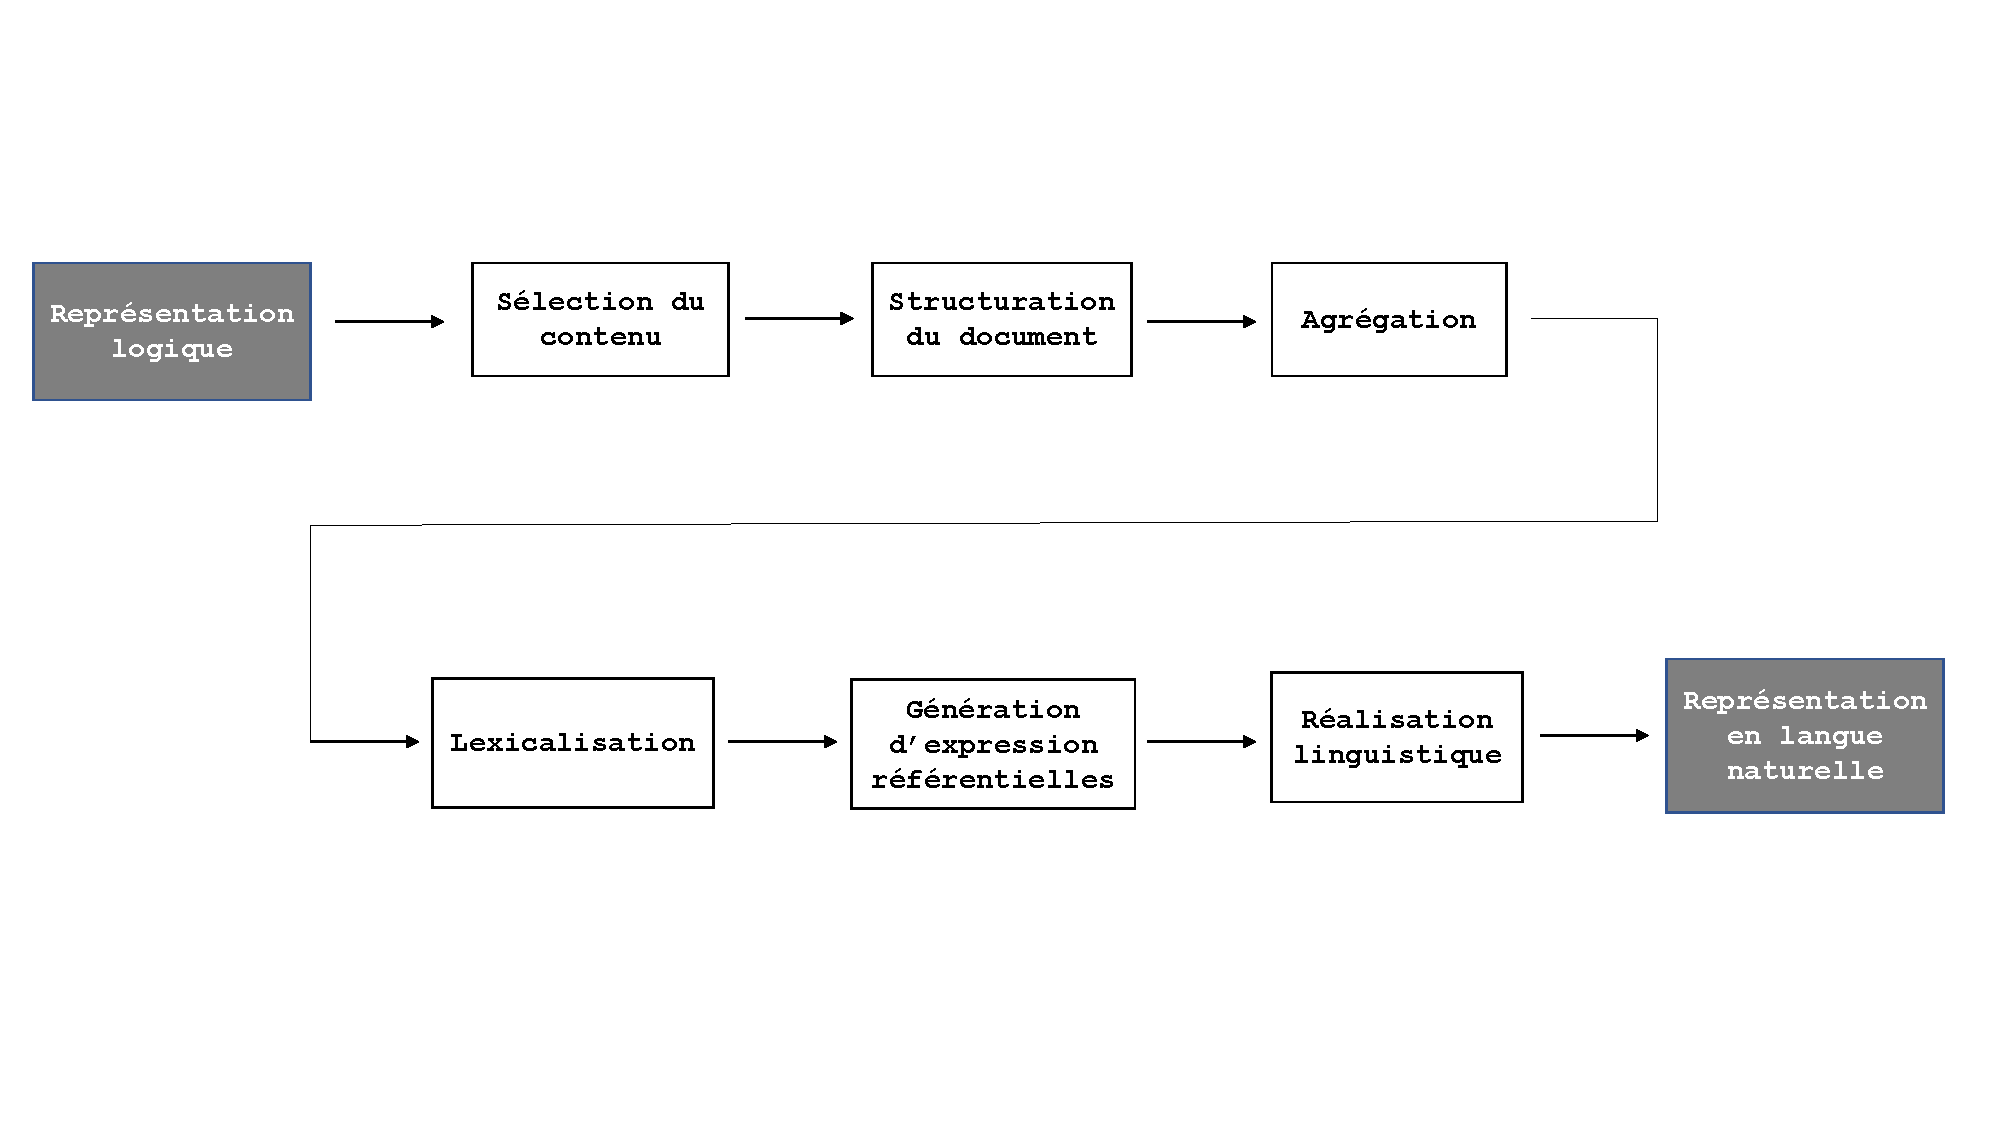
\includegraphics[width=1\textwidth, trim = {0cm 0cm 0cm 0cm},clip]{ch2/figs/pipeline.pdf}
	\caption{Pipeline classique}
	\label{fig:Pipeline}
\end{figure}

\FL{ça vaut pas la peine de faire des sous-sections numérotées pour des petits paragraphes comme ça. commence chaque paragraphe par le nom de l'étape que tu décris, comme ça on voit clairement la structure. tu peux même les mettre en gras pour faciliter la lecture}

Un système de \ac{GAT} doit départir les informations qui seront dans le texte de celles qui n'y seront pas. Il s'agit donc de déterminer ce qui est pertinent dans les données brutes. Par exemple, si on souhaite générer le compte rendu d'un match de soccer, on ne voudrait probablement pas mentionner toutes les passes et toutes les fautes commises durant ce match, même si ces informations figurent dans les données de base. La \textbf{sélection du contenu} dépend aussi beaucoup du public à qui le texte est adressé et de l'objectif du texte: on ne présente pas la même information à un expert et à un novice. Dans le cas d'un compte rendu sportif, par exemple, on pourrait vouloir adapter le texte en fonction de l'équipe préférée du lecteur.

Ensuite, on crée \textbf{le plan du texte} à générer. Il s'agit de décider dans quel ordre présenter les informations sélectionnées. Cette étape est une représentation ordonnée et structurée du message à transmettre. Reprenons l'exemple du soccer. En fonctions des données choisies, le texte devra débuter par les informations générales liées au match (où et quand le match s'est déroulé), suivi du nom des équipes qui s'opposaient, de qui a gagné, puis des faits saillants du match.

\textbf{L'agrégation} est l'étape où on combine des messages en une seule phrase afin de rendre le texte plus fluide et agréable à lire. Les messages sélectionnés dans le plan (structuration du document) n'ont pas à être exprimé dans des phrases individuelles si on est capable de les combiner \citep{ChengCapturingInteractionAggregation2000}. Bref, cette étape sert à éviter la redondance et un style trop télégraphique.

La \textbf{lexicalisation} est l'étape où l'on traduit les données non-linguistiques en langue naturelle. Il s'agit de choisir les lexèmes qui seront utilisés pour transmettre le message voulu. Comme il existe naturellement plusieurs manières de rendre une même idée en mots, cette tâche peut devenir assez complexe si on veut que le système tienne compte des subtilités de la langue. La sélection des lexies peut ainsi se faire à divers niveaux d'abstraction. Un niveau plus abstrait requière plus de travail et est plus complexe à mettre en place. Toutefois, il génère plus de possiblités au moment de la réalisation. \cite{ElhadadFloatingConstraintsLexical1997} prônaient une approche en faveur de la lexicalisation profonde. Par exemple, un système de \ac{GAT} permettant une lexicalisation profonde pourrait générer les paraphrases suivantes: \form{Paul marque un but spectaculaire pendant la deuxième période} et \form{Paul réussi un but à couper le souffle lors de la seconde période}.

\textbf{La génération d'expressions référentielles} est très similaire à la lexicalisation car on choisit comment se réaliseront certaines entités. Le but est de s'assurer que le lecteur puisse distinguer correctement chaque entité. Pour cela, il faut trouver la meilleure façon de référer à une entité. Pour ces raisons, on l'appelle souvent \scare{l'étape discriminatoire}. Continuons avec l'exemple du soccer. Cette étape du processus nous permet de référer à une même joueur de diverses manières dans le texte. Par exemple: l'attaquant, la jeune recrue, Joe McCain, McCain, Little-Joe, le récipiendaire du prix McKenna, etc.

La dernière étape est \textbf{la réalisation linguistique}. Lorsque tous les mots et les expressions référentielles ont été choisis, on peut réaliser le texte final. Cette tâche implique l'application de traits morpho-syntaxiques aux lexèmes et la linéarisation des structures. Elle inclut aussi l'insertion des mots fonctionnels (auxiliaires, déterminants,etc.) et la ponctuation. Cette étape du processus nous intéresse particulièrement, donc nous allons élaborer sur celle-ci.



%%%%%%%%%%%%%%%%%%%%%%%%%%%%%%%%%%%%%%%%%%%%%%%%%%%%%%%
% --------- R É A L I S A T I O N   ---------
%%%%%%%%%%%%%%%%%%%%%%%%%%%%%%%%%%%%%%%%%%%%%%%%%%%%%%%


\section{Réalisation}

Puisque nous avons maintenant traité du processus global de \ac{GAT} et des différentes méthodes de réalisation, nous pouvons entrer dans les détails de la tâche qu'est la réalisation linguistique, dans laquelle s'insère notre travail.

Tel qu'explicité à la figure~\ref{fig:Pipeline}, la réalisation est la dernière étape dans le processus de \ac{GAT}. Toutefois, pour beaucoup de chercheurs, elle ne représente pas uniquement les tâches décrites précédemment. Il règne en effet un certain flou autour de ce qui constitue la réalisation. Pour certains, elle correspond exactement à la description de la réalisation que nous fournissons en \ref{ppc}. On appellera cela la réalisation de surface, puisque la réalisation se fait à partir d'un input beaucoup plus près du texte (des structures syntaxiques lexicalisées). Pour d'autres, la réalisation se fait à partir de données plus abstraites, en amont de la lexicalisation. Ce type de réalisation plus profonde prend généralement en input des structures pré-syntaxiques. On les appellera des réalisateurs profonds. Dans ces systèmes, les informations lexicales et grammaticales seront encodées dans des dictionnaires et des grammaires plus complexes permettant de traiter l'interface sémantique-syntaxe. Finalement, ces systèmes profonds sont généralement liés à une théorie linguistique leur permettant de modéliser le langage et de l'encoder dans un système informatique.

\subsection{Types d'approches}

Il existe traditionnellement trois types d'approches pour la réalisation.

Nous nommerons d'abord, l'\textbf{approche à base de patrons}. Elle est généralement utilisée pour produire du texte dans des domaines spécifiques comme la météo ou les sports. Cette approche réduit la variation linguistique à un minimum puisque chaque réalisation de texte se fait à partir d'un moule fixe \citep{mcroy_channarukul_ali_2003}. Les phrases en \ref{template}, provenant de l'article de \cite{gatt18}, démontrent comment de tels patrons s'utilisent.

\ex. \label{template}
	\a.\$player scored for \$team in the \$minute minute. \label{a.}
	\b. Ivan Rakitic scored for Barcelona in the 4th minute.

En \ref{a.}, le patron contient trois variables, marquées par les \$. Celles-ci peuvent être respectivement comblées par un nom de joueur, suivi d'un nom d'équipe et d'une indication temporelle. L'avantage de cette approche est qu'on peut prévoir exactement ce qui sera généré et on diminue, par le fait même, les risques d'erreurs. L'inconvénient est que cette approche est très rigide et laisse place à quasi aucune paraphrase. Cependant, les réalisateurs à base de patrons peuvent être complémentés par des règles de grammaire, ce qui les rend plus flexibles. Toutefois, puisqu'ils sont codés à la main, ces sytèmes ont l'inconvénient d'être coûteux à développer. \cite{gatt18} soulignent qu'ils peuvent aussi être combinés à de l'apprentissage machine pour automatiser l'écriture des patrons, ce qui rend la tâche moins coûteuse. D'ailleurs, la combinaison d'approches est une démonstration de l'affaissement des frontières (création de systèmes hybrides) entre les méthodes traditionnelles de réalisation.


Ensuite, il y a l'approche textbf{basée sur des règles grammaticales}. Celles-ci s'emploient autant dans les domaines spécifiques (météo, sport, etc.) que les domaines généraux (conversation libre). Ces systèmes de réalisation se prêtent bien à la langue courante puisqu'ils sont conçus pour représenter le langage à travers des règles de grammaire. Cependant, les grammaires et les dictionnaires nécessaires au bon fonctionnement de cette approche sont codés manuellement, ce qui demande du temps et des ressources.


Finalement, il y a les \textbf{méthodes statistiques}. On peut les utiliser pour filtrer les sorties d'un système à l'aide d'un modèle probabiliste qui déterminera quel output est la meilleur candidat \citep{LangkildeForestbasedStatisticalSentence2000} (aussi appellée l'approche \emph{generate-and-filter}). On peut aussi développer un modèle probabiliste permettant à un système de \ac{GAT} d'apprendre automatiquement les règles nécessaires pour générer du texte \citep{WhiteMinimalDependencyLength2012}. Les méthodes statistiques diminuent considérablement la charge de travail manuelle \citep{LangkildeForestbasedStatisticalSentence2000}.

Considérant les approches que nous venons de présenter, une question surgit quant à la nécessité de continuer à développer des méthodes à base de règles lorsqu'on peut sauver du temps et employer des méthodes probabilistes. À ce sujet, \cite{BelzSystemBuildingCost2009} se sont demandé si le temps gagné en automatisant la réalisation se faisait au détriment de la qualité et si c'était le cas, à quel point. Leur évaluation consistait à tester les deux méthodes en leur demandant de faire la même tâche. Ils ont ainsi considérer la qualité des textes via une évaluation humaine, puis une évaluation métrique faite automatiquement. Suite à l'analyse, ils nous expliquent que les évaluations humaines pointaient en faveur des systèmes à base de règles et que certaines évaluations métriques surévaluaient le système statistique et sous-évaluaient le système à base de règles.

Reiter s'est aussi penché sur la question et en a fait un survol dans un article tiré de son blog.\footnote{\url{https://ehudreiter.com/2016/12/12/nlg-and-ml/}, 12-03-18} Selon lui, même si les systèmes d'apprentissage automatique produisent généralement de bons textes, ils en génèrent occasionnellement des bizarretés. Ce comportement n'est pas approprié dans des domaines professionnels où des utilisateurs comptent sur la qualité des textes, entre autre, car ils prendront potentiellement des décisions en fonction des textes générés. De plus, les systèmes basés sur des méthodes statistiques ont souvent plus de difficulté à corriger les incongruités. En revanche, les systèmes à base de règles permettent de cerner les problème avec plus de facilité et de les corriger. Cependant, Reiter termine son blog en soulignant que la \ac{GAT} a aussi beaucoup à gagner de l'emploi des méthodes statistiques. Il suggère qu'on se serve d'elles pour automatiser des étapes du processus de réalisation (à base de règles).

%%%%%%%%%%%%%%%%%%%%%%%%%%%%%%%%%%%%%%%%%%%%%%%%%%%%%%%
% --------- R É A L I S A T E U R   S U R F A C E ---
%%%%%%%%%%%%%%%%%%%%%%%%%%%%%%%%%%%%%%%%%%%%%%%%%%%%%%%

\subsection{Réalisateurs de surface}

Dans cette section, nous présenterons trois réalisateurs de surface connus: SimpleNLG, JSrealB et RealPro.

\subsubsection{SimpleNLG}
SimpleNLG \citep{GattSimpleNLGRealisationEngine2009} est un réalisateur de surface pour l'anglais écrit en java. Le texte est réalisé à partir d'une structure syntaxique déjà lexicalisée encodée en XML. Par la suite, le réalisateur effectue les opérations morphologiques nécessaires (flexion, dérivation, ajout d'auxiliaires, gestion de l'accord) tout en linéarisant le texte.

Puisqu'il s'agit d'un réalisateur à base de règles, SimpleNLG est doté d'une grammaire et d'un dictionnaire. Ce dernier encode les propriétés syntaxiques et morphologiques des unités lexicales. Puis, le module grammatical contient des règles permettant le passage de la syntaxe à la morphologie.

SimpleNLG sépare son processus de réalisation en quatre étapes. Premièrement, les lexèmes compris dans la structure d'input sont mis en correspondance avec leurs entrées de dictionnaire. Deuxièmement, on détermine les traits spécifiques des lexèmes. Troisièmement, on combine les lexèmes en créant des syntagmes de plus en plus larges, jusqu'à ce que l'entièreté de la phrase forme un syntagme phrastique. Finalement, les règles morphologiques sont appliquées et les lexèmes sont accordés afin d'obtenir les formes fléchies.

D'ailleurs, SimpleNLG a été traduit dans plusieurs langues dont l'espagnol \citep{RamosSotoAdaptingSimpleNLGSpanish2017}, l'italien \citep{MazzeiSimpleNLGITadaptingSimpleNLG2016}, le français \citep{VaudryAdaptingSimpleNLGBilingual2013}, le portugais \citep{deOliveiraAdaptingSimpleNLGBrazilian2014} et l'allemand \citep{BollmannAdaptingSimpleNLGGerman2011}.

La figure \ref{simplenlg} illustre l'input nécessaire permettant de réaliser la phrase \form{Refactoring is needed}. Elle provient du GitHub de SimpleNLG.\footnote{\url{https://github.com/simplenlg/simplenlg/blob/master/docs/XMLRepresentationOfTextSpecifications.pdf}}

\begin{lstlisting}[language=Xml, caption=Structure d'input dans SimpleNLG, label=simplenlg]
<Document>
  <child xsi:type="SPhraseSpec">
    <subj xsi:type="VPPhraseSpec" FORM="PRESENT_PARTICIPLE">
      <head cat="VERB">
        <base>refactor</base>
      </head>
    </subj>
    <vp xsi:type="VPPhraseSpec" TENSE="PRESENT" >
      <head cat="VERB">
        <base>be</base>
      </head>
      <compl xsi:type="VPPhraseSpec" FORM="PAST_PARTICIPLE">
        <head cat="VERB">
          <base>need</base>
        </head>
      </compl>
    </vp>
  </child>
</Document>
\end{lstlisting}

\subsubsection{JSrealB}
JSrealB (pour \emph{JavaScript Realiser Bilingual}) \citep{DBLP:conf/enlg/MolinsL15} est conçu pour les programmeurs web. Ce réalisateur génère des expressions et phrases bien formées qui peuvent être formattées en HTML pour ensuite être utilisées dans un fureteur. JSreal peut aussi s'employer seul à des fins purement linguistiques. Généralement, les spécificités de JSreal sont assez similaires à celles de SimpleNLG \citep{GattSimpleNLGRealisationEngine2009}.

Pour générer du texte, JSrealB prend en input des structures syntaxiques lexicalisées. La construction de la phrase découle de l'application de règles syntaxiques et morphologiques déclenchées par les lexèmes. JSrealB fonctionne aussi avec un dictionnaire et une grammaire. Son dictionnaire définit la catégorie des lexèmes qui le peuple et leurs traits lexicaux (genre, nombre, irrégularités, etc.). La grammaire de JSrealB contient des règles morpho-syntaxiques qui lui permettent de faire l'accord entre les constituants. Finalement, il existe aussi une version bilingue de JSrealB \citep{MolinsJSrealBBilingualText2015} qui incorpore le français et l'anglais. L'input qu'illustre la figure \ref{jsreal} permet au réalisateur de générer la phrase: \form{The cat sat on the oach}. Cet exemple est tiré du GitHub de JSrealB.\footnote{\url{https://github.com/rali-udem/JSrealB}}

\begin{lstlisting}[language=Xml, caption=JSreal, label=jsreal]
JSrealLoader({
        language: "en",
        lexiconUrl: URL.lexicon.en,
        ruleUrl: URL.rule.en,
        featureUrl: URL.feature
    }, function() {
    QUnit.test( "Sentence EN", function( assert ) {
        assert.equal(
            S(
                NP(D("the"), N("cat")),
                VP(V("sit"), PP(P("on"), NP(D("the"), N("coach")))).t("ps")
            )
\end{lstlisting}
		
\subsubsection{RealPro}
RealPro \citep{LavoieFastPortableRealizer1997} est implémenté en C++. Il est le plus profond des réalisateurs de surface préséntés ici. Il prend en input des arbres de dépendances, ce qui le distingue des deux autres systèmes qui utilisent des arbres de constituants \citep{DBLP:conf/enlg/MolinsL15,GattSimpleNLGRealisationEngine2009}. Rapidement, un arbre de dépendance est non-linéarisé dont les arcs et les noeuds sont identifiés. Les noeuds sont des lexèmes, donc la lexicalisation a déjà eu lieu. On appelle ça un arbre syntaxique car les branches liant les noeuds entre eux correspondent à des relations syntaxiques. Seul les mots pleins de sens figurent dans l'input (cela exclue les déterminants, prépositions, etc.). Cette architecture est basée sur la \ac{TST} \citep{melcuk1988}. Nous ferons une petite paranthèse ici, car nous parlerons souvent de la \ac{TST} dans ce mémoire. C'est une théorie linguistique qui a fait ses preuves en matière de \ac{GAT} si on se fie à RealPro \citep{LavoieFastPortableRealizer1997} que nous présontons ici et FORGe \citep{MilledemoFORGePompeu2017} ou MARQUIS \citep{WannerMARQUISGENERATIONUSERTAILORED2010} qui l'utilise aussi. De plus, \cite{Vicentegeneracionlenguajenatural2015} mentionne ce cadre théorique comme étant une bonne interface pour modéliser le langage dans une système de \ac{GAT}.

Brièvement, il s'agit d'une théorie qui divise le langage en quatre niveaux de représentations majeurs: sémantique, syntaxique (profonde et de surface), morphologique (profonde et de surface), phonologique (profonde et de surface) -- ce dernier étant court-circuité pour la génération de texte écrit. Pour plus de détails concernant les arbres de dépendances et la \ac{TST}, voir le chapitre~\ref{chapgendr}.

RealPro a deux grammaires qui permettent successivement de passer d'une représentation profonde à une représentation de surface, puis de celle-ci à une linéarisation morphologique de l'input. Pour effectuer toutes les transitions, le système fait aussi appel à un dictionnaire qui encode les propriétés lexicales et morphosyntaxiques des unité. Le graphique \ref{fig:RealPro} démontre l'intéraction de ces deux ressources pour réaliser le texte.

\begin{figure}[htb]
	\centering
	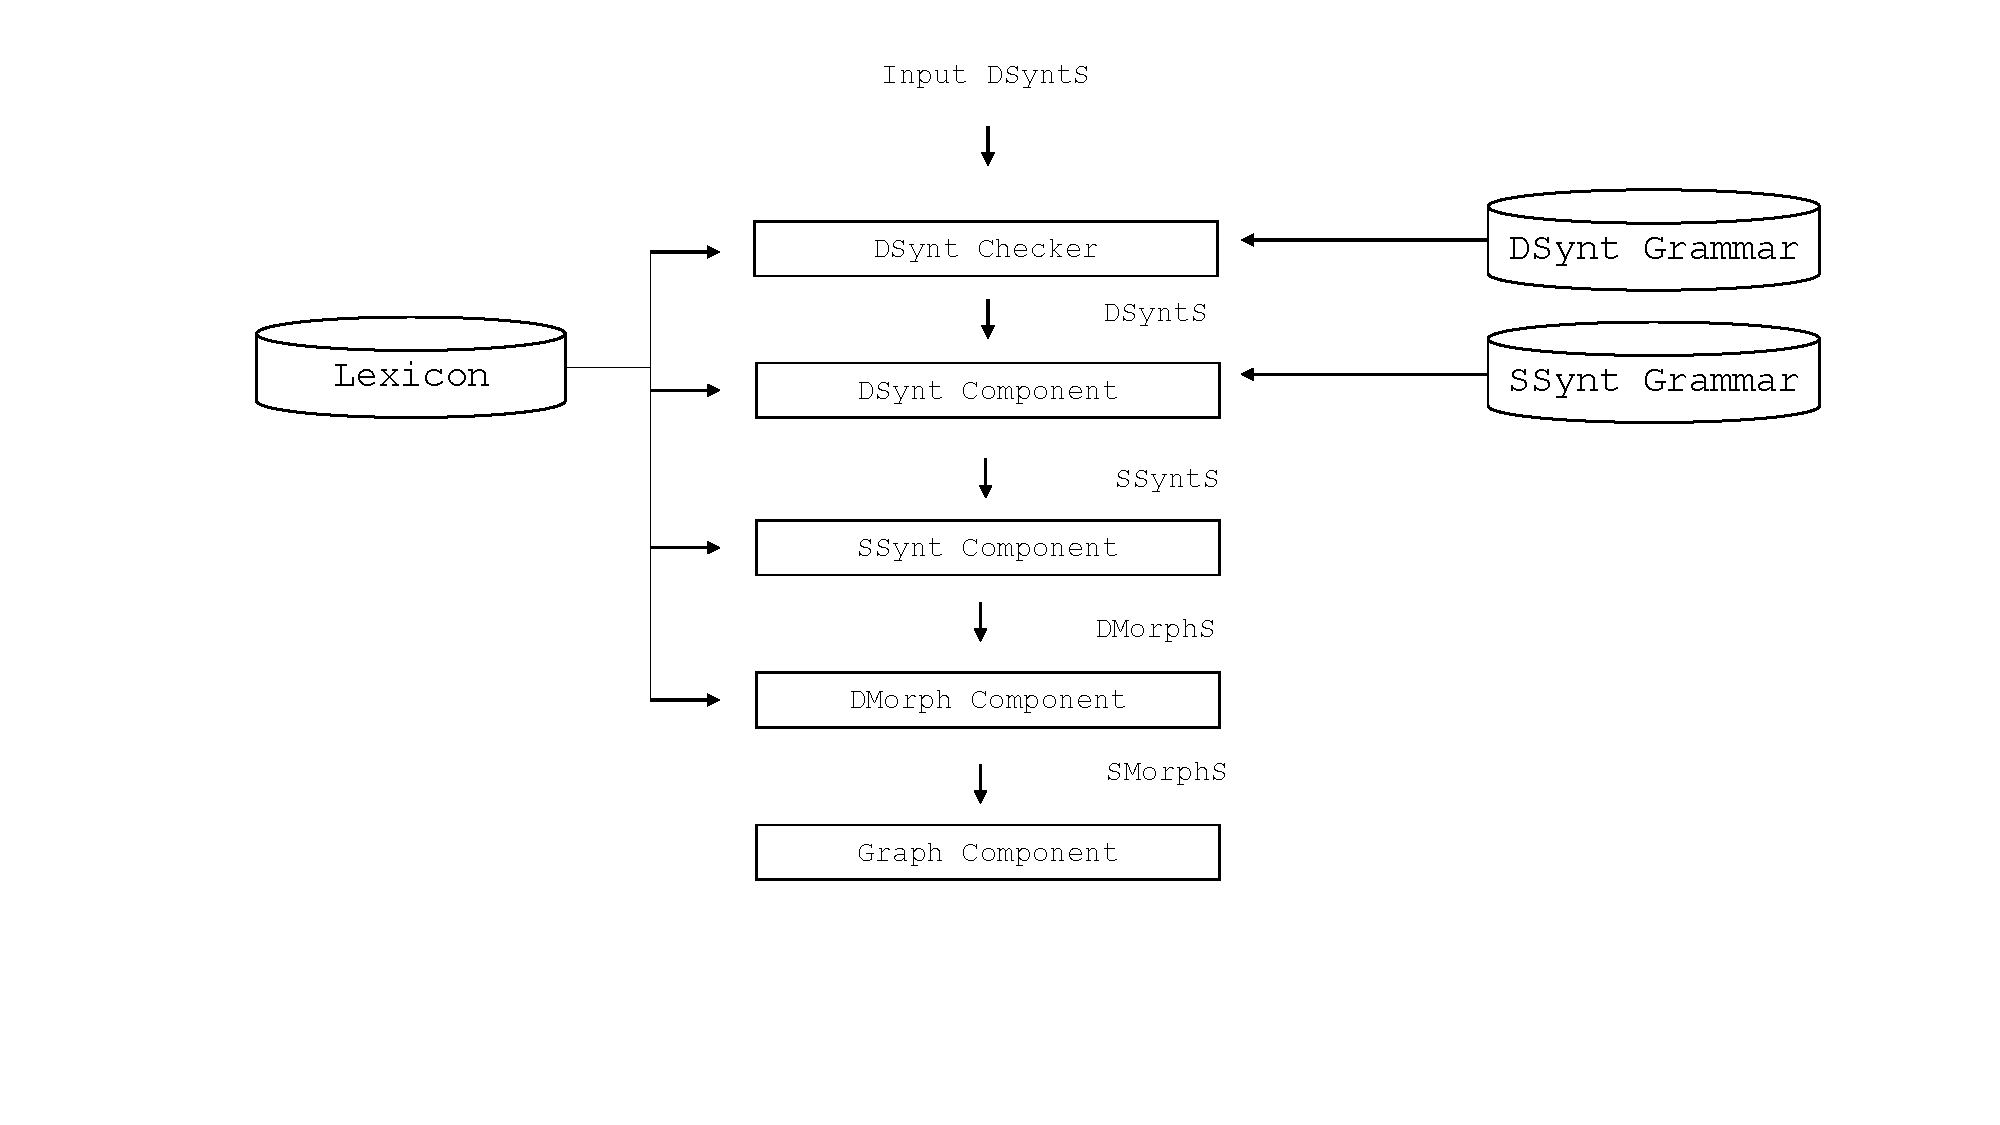
\includegraphics[width=1\textwidth, trim = {0cm 0cm 0cm 0cm},clip]{ch2/figs/realpro.pdf}
	\caption{RealPro}
	\label{fig:RealPro}
\end{figure}

La figure \ref{lst:realpro} illustre un arbre de dépendance (l'input) représentant la phrase \form{March had some rain days}. Ce qu'on peut retirer de cet exemple que \lex{have1} est la racine de l'arbre et que \lex{march} puis \lex{day} en sont les actants. Ceux-ci appartiennent à des classes nominales et on peut voir qu'il y a des contraintes sur certains noeuds. La lexie \lex{day} demande que le module morphologique fléchisse la lexie au pluriel. Cet exemple provient de \cite{ReiterBuildingNaturalLanguage2000}.

\begin{minipage}{\linewidth}
\begin{lstlisting}[language=Xml, caption=Input, label=lst:realpro]
HAVE1 [tense:past]
(I March [class:proper-noun]
II day [class:common-noun numberpl]
(ATTR rainy [class:adjective]))
\end{lstlisting}
\end{minipage}
%%%%%%%%%%%%%%%%%%%%%%%%%%%%%%%%%%%%%%%%%%%%%%%%%%%%%%%
% --------- R É A L I S A T E U R    P R O F O N D  ---
%%%%%%%%%%%%%%%%%%%%%%%%%%%%%%%%%%%%%%%%%%%%%%%%%%%%%%%

\subsection{Réalisateurs profonds}

Les réalisateurs profonds prennent généralement en input des structures plus abstraites, ce qui a pour conséquence plus de variation linguistique. Comme les réalisateurs profonds incorporent généralement la lexicalisation, un input peut généralement produire divers outputs \citep{PolguerePourmodelestratifie}. Le \scare{pouvoir paraphrastique} de ces systèmes permet donc au réalisateur de tenir compte de toute la richesse langagière d'une langue. Dans le pipeline classique, comme nous l'avons vu à la section \ref{ppc}, la lexicalisation est opérée avant la réalisation. Cet ordre a pour conséquence que les inputs fournis au réalisateur sont déjà lexicalisés et cela restreint grandement les réalisations possibles (puisque les lexèmes incorporent des propriétés de combinaitoires bien précises autours desquelles la phrase doit s'articuler). 

Dans cette section, nous présenterons les réalisateurs profonds suivants: KPML, SURGE, FORGe et MARQUIS.

\subsubsection{KPML}
KMPL \citep{BatemanEnablingTechnologyMultilingual1997} est un réalisateur multilingue issu du système PENMAN \citep{PenmanOverview}. La théorie linguistique sous-jacente à ce système est la \ac{SFG} \citep{MatthiessenSystemicfunctionalgrammar1997}, qui postule que les choix linguistiques sont déclenchés par l'exécution de fonctions grammaticales. D'un point de vue multilingue, les différentes langues issues de KPML partagent la majorité des fonctions grammaticales. Ces fonctions forment le c\oe{}ur du système, mais il existe aussi quelques fonctions propres à chaque langue pour réaliser les phénomènes linguistiques spécifiques à chacune.

La grammaire de ce système est implémentée à la manière d'un réseau orienté. Chaque intersection dans le réseau correspond à un choix grammatical à faire entre différents traits fonctionnels. Ces choix deviennent de plus en plus précis lorsqu'on avance dans le réseau. Ainsi, la forme de surface d'un input donné est la conséquence du parcours de ces réseaux.

Les informations comprises dans les inputs de ce système sont d'ordre sémantique et syntaxique. Ainsi, l'input de KPML est un\ac{SPL}, ce qui est une une matrice d'attributs et de valeurs. La figure \ref{kpml} représente à quoi ressemble un \ac{SPL} et elle est issue de \cite{ReiterBuildingNaturalLanguage2000}. Elle représente la phrase \form{March had some rainy days}.

\begin{minipage}{\linewidth}
\begin{lstlisting}[language=Xml, caption=SPL: input de KPML, label=kpml]
(S1 \ generalized-possession
  :tense past 
	:domain (N1 \ time-interval
	            :lex march
							:determiner zero)
	:range (N2 \ time-interval
	           :number plural
						 :lex day
						 :determiner some
						 :property ascription
						 (A1 \ quality :lex rainy)))
\end{lstlisting}
\end{minipage}

\subsubsection{SURGE}
SURGE, qui signifie \emph{Systemic Unification Realisation Grammar of English}, est une grammaire de l'anglais \citep{Elhadad98surge:a} qui est écrite en \ac{FUF}: une grammaire basée sur \acf{FUG} \citep{KayFunctionalUnificationGrammar1984}. \ac{FUF} est un langage de programmation créé pour construire des grammaires d'unification informatisées.

SURGE prend en input des arbres thématiques non linéarisés dont les noeuds sont des unités sémantiques pleines (donc ça exclut les prépositions,etc.). Ces arbres sont représentés comme des structures de traits encodé dans le formalisme \ac{FUF}. Ces structures de traits sont appellées des \ac{FD}. Il s'agit d'ensemble de paires d'attributs-valeurs qui peuvent être sucessivement enchâssées. Les entrées lexicales et leurs propriétés sont directement encodées dans les \ac{FD} ce qui fait en sorte que SURGE n'a pas besoin de dictionnaire. Chaque constituant se fait attribuer une catégorie syntaxique et c'est grâce à ces traits que la grammaire sait comment unifier la phrase.

Dans ce système, la grammaire est aussi décrite en termes de \ac{FD}. Ainsi, réaliser du texte, SURGE prend en entrée à la fois les \ac{FD} du sens de la phrase désirée et les \ac{FD} représentant les règles de grammaire du système afin d'unifier les structures. Le résultat est une structure d'entrée enrichie par des spécifications grammaticales (syntaxique et morphologique). Cela permet au réalisateur de passer à l'étape suivante qui est la linéarisation. SURGE applique ainsi les traits morphologiques en fonction des spécifications encodées lors de l'unification. L'output est une phrase anglaise exprimant le sens de la \ac{FD} en fonction des contraintes imposées par la grammaire.

Nous reprenons encore un exemple tiré de \cite{ReiterBuildingNaturalLanguage2000}: \form{March had some rainy days}.

\begin{minipage}{\linewidth}
\begin{lstlisting}[language=Xml, caption=FD: input de Surge, label=surge]
((cat clause)
 (proc ((type possessive)))
 (tense past)
 (partic ((possessor ((cat proper) head ((lex "March"))))
					(possessed ((cat common) head ((lex day)))
											(describer ((lex rainy)))
											(selective yes) (number plural)))))
\end{lstlisting}
\end{minipage}

\subsubsection{MARQUIS}\label{sectionmarquis}
Comme RealPro, MARQUIS est basé sur la \ac{TST}, mais contrairement aux autres systèmes présentés ici, MARQUIS n'est pas qu'un réalisateur profond. Il s'agit d'un système de \ac{GAT} complet qui effectue toutes les étapes du processus de génération automatique de texte (voir \ref{ppc}). Cependant, nous ne nous intéresserons ici qu'à son module de réalisation profonde.\citep{Lareau2007TowardsAG} Pour plus d'informations concernant le pipeline complet de MARQUIS, voir \citep{WannerMARQUISGENERATIONUSERTAILORED2010}. 

Le but du projet MARQUIS était de générer, à partir de données brutes, des bulletins météorologiques multilingues sur la qualité de l'air. Ces bulletins sont générés en fonction de l'utilisateur. Autrement dit, ceux-ci se créent des profils avec leurs informations personelles et cela permet à MARQUIS de réaliser du texte en fonction de leur niveau de connaissance du domaine et de leurs besoins de santé. Le tout est fait à partir d'un input conceptuel partagé par toutes les langues traitées par MARQUIS (l'anglais, l'allemand, l'espagnol, le catalan, le portugais, le français, le finnois et le polonais). 

La figure \ref{fig:marquis} illustre le processus de réalisation que MARQUIS entreprend pour générer du texte. On peut y voir que le système prend en input des graphes conceptuels et qu'il produit du texte. Concrètement, pour arriver à la réalisation finale, MARQUIS prend la structure \#1 et à l'aide de dictionnaires et de grammaires, il construit un nouveau graphe correspondant à la structure précédente et ainsi de suite jusqu'à ce qu'il arrive à la dernière représentation. 

\begin{figure}[htb]
	\centering
	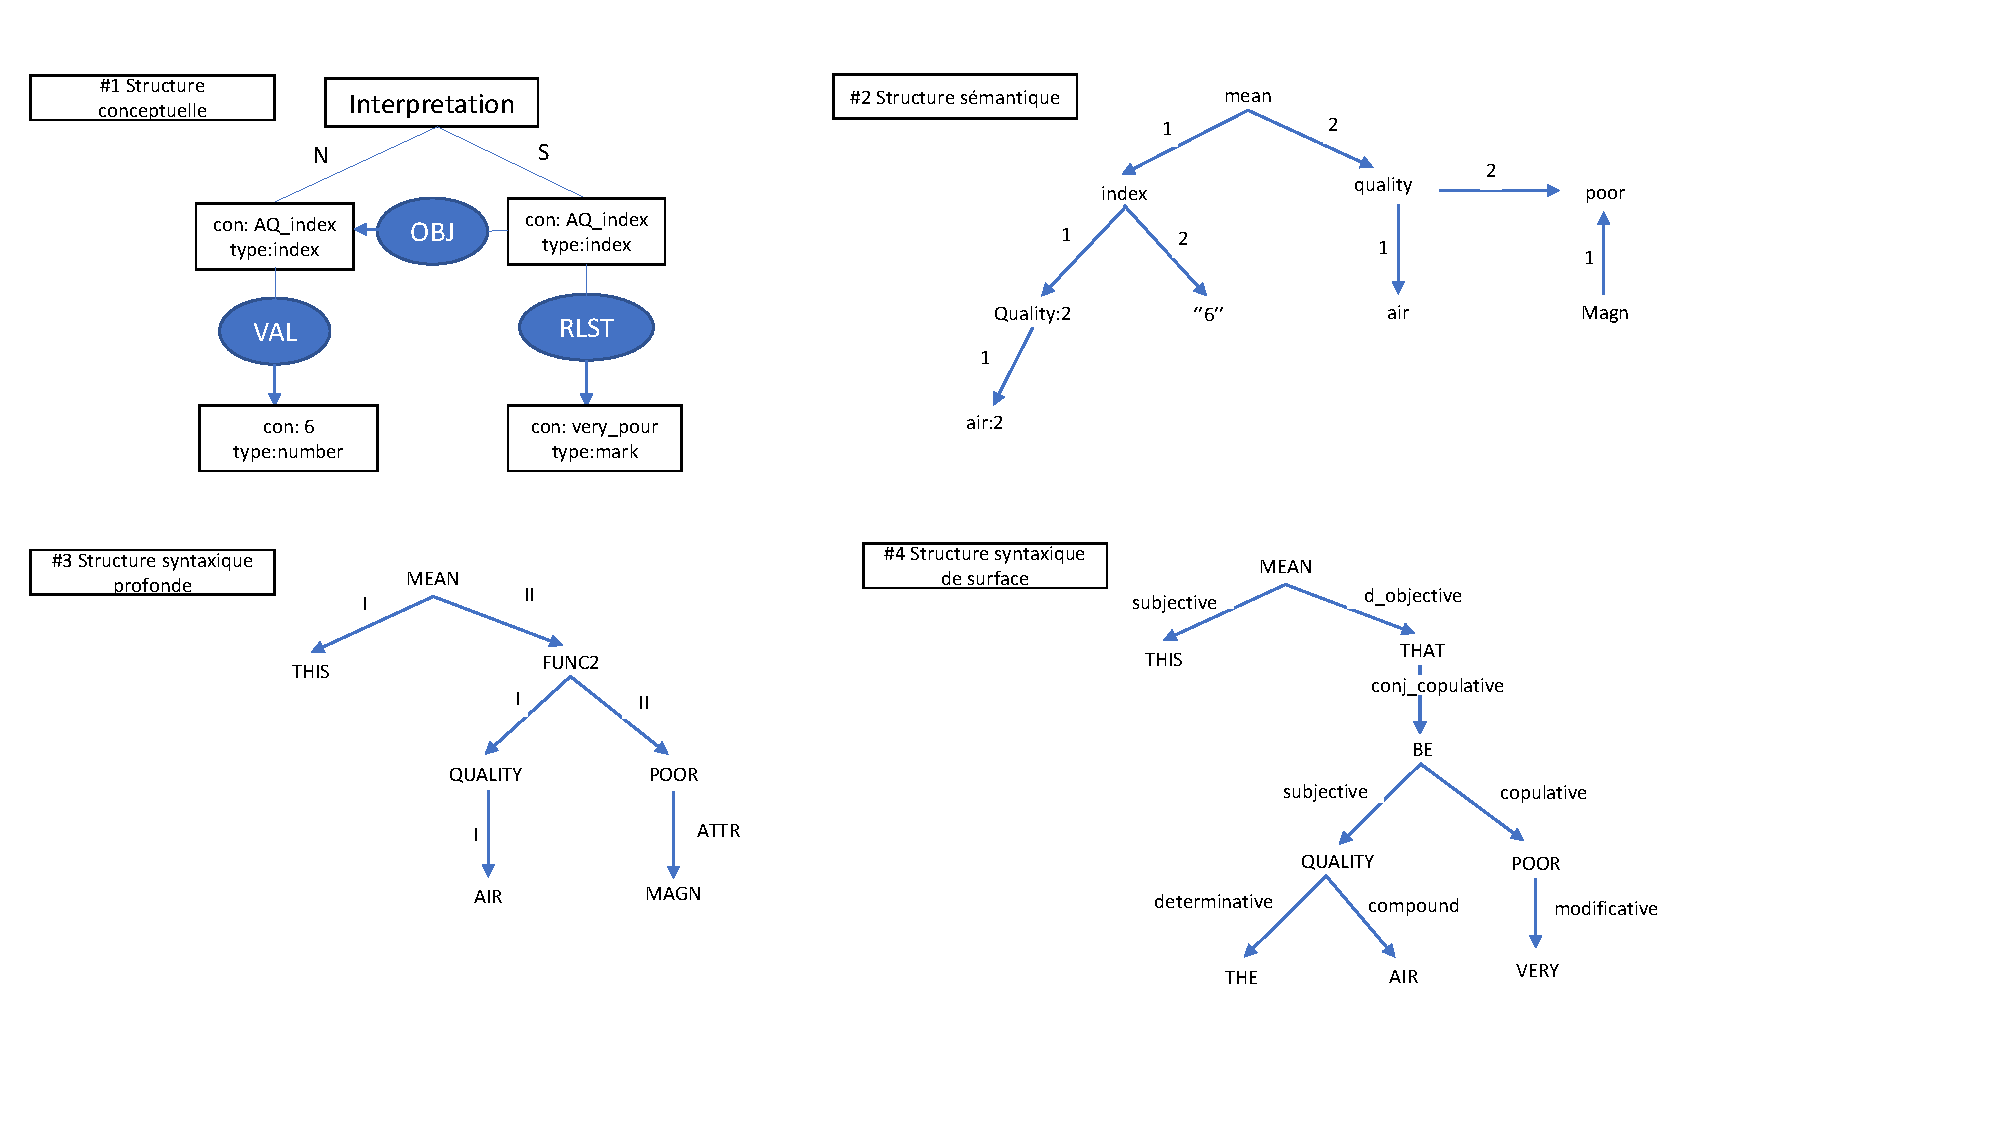
\includegraphics[width=1\textwidth, trim = {0cm 0cm 0cm 0cm},clip]{ch2/figs/marquis.pdf}
	\caption{Pipeline de MARQUIS}
	\label{fig:marquis}
\end{figure}

Nous expliquerons brièvement les mécanismes qui permettent la transition d'une représentation à une autre puisque le tout sera mieux expliquée à la section \ref{secsemsynt}. Alors, il faut d'abord que le système analyse la structure conceptuelle. Ensuite les règles de transduction permettent de passer de la représentation conceptuelle à la représentation sémantique. Le passage des unités conceptuelles aux unités sémantique se fait via l'entremise des dictionnaires respectifs. On a alors une structure sémantique. MARQUIS prendra ce graphe pour en dériver un arbre de dépendances syntaxique profond grâce aux règles de transduction de cette interface. La mise en correspondance d'unités sémantiques et lexicales est opérée grâce au dictionnaire sémantique (\emph{semanticon}) et lexical (\emph{lexicon}) ainsi qu'au dictionnaire de fonctions lexicales. Finalement, les autres transitions de représentations sont assurées par des règles de transductions successives et les informations contenues dans le lexicon. La figure \ref{fig:reglesdict} démontre ces rouages.

\begin{figure}[htb]
	\centering
	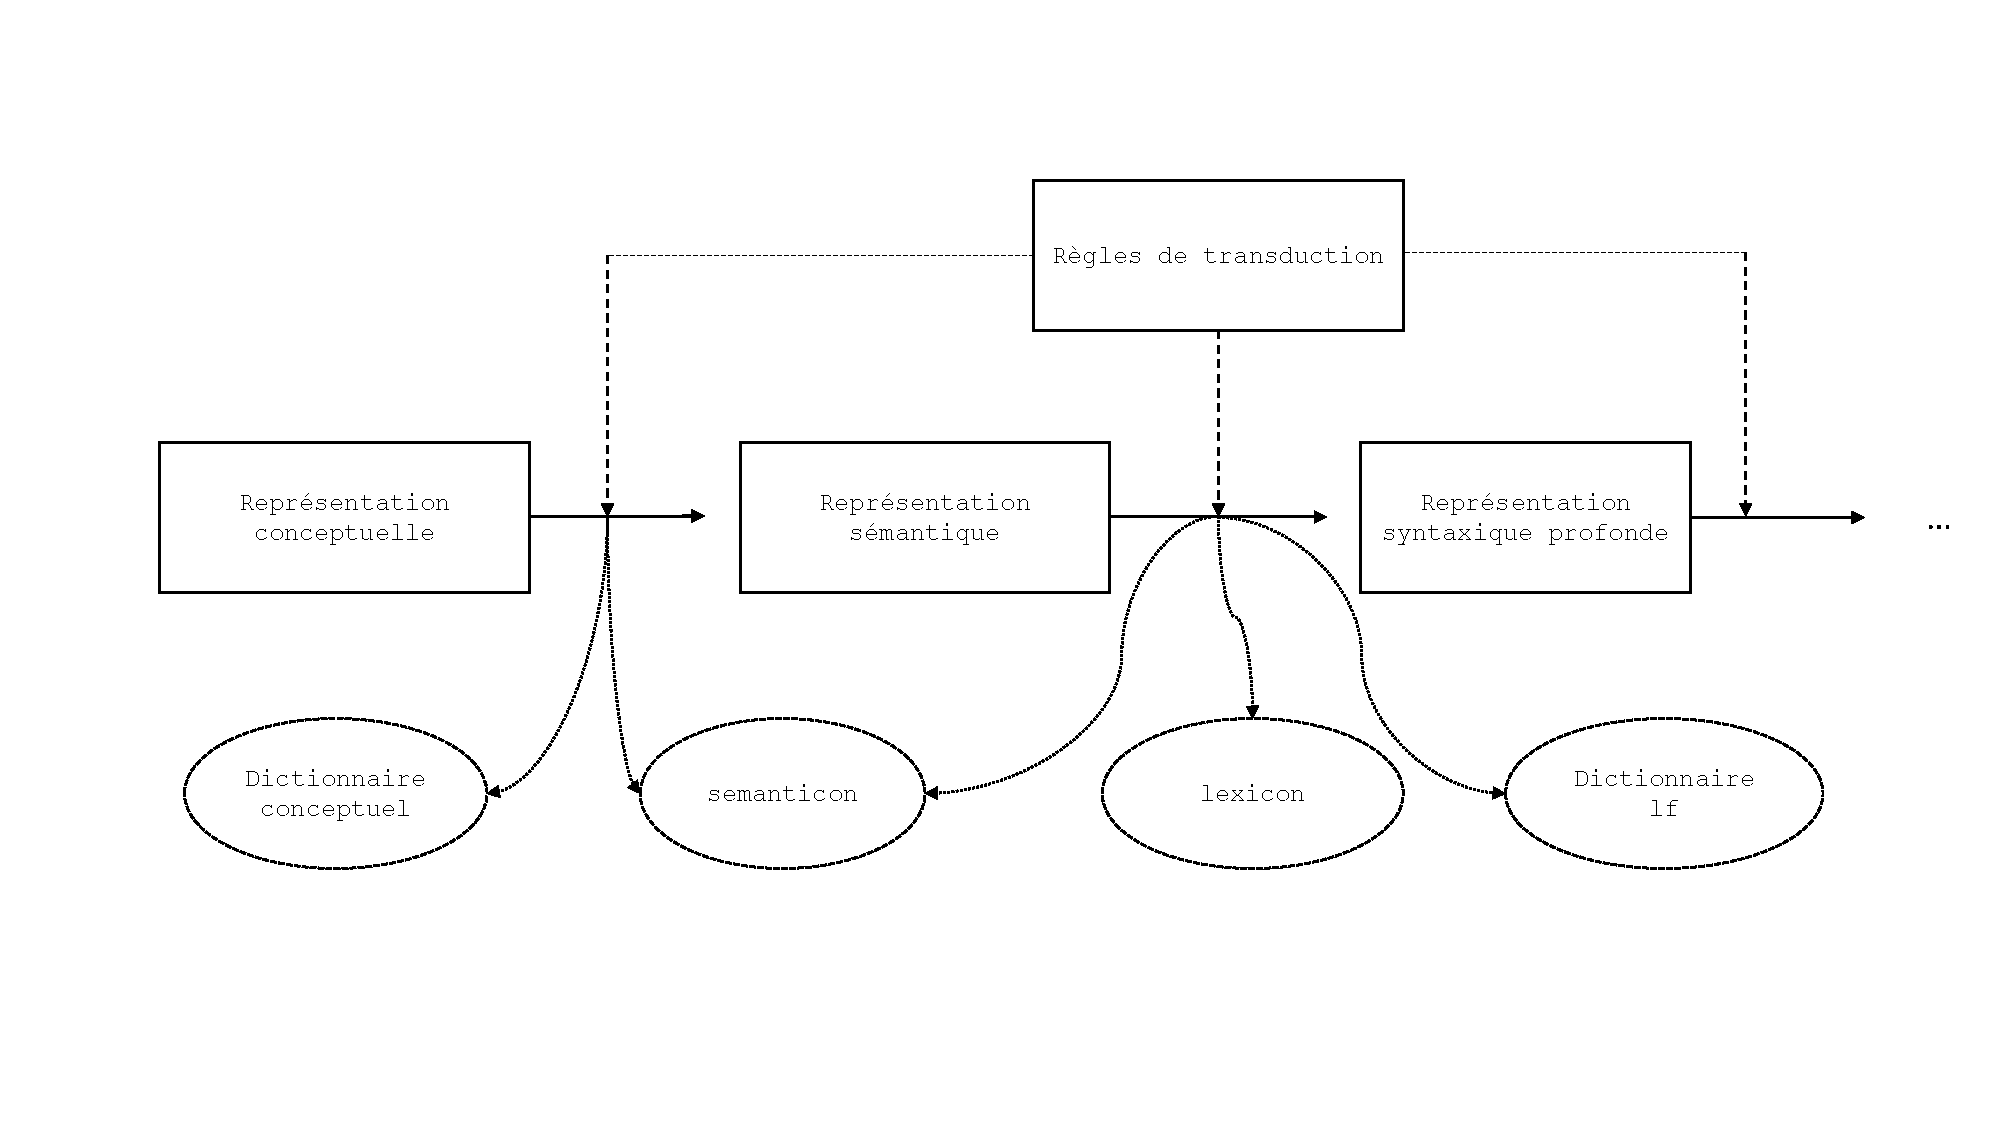
\includegraphics[width=1\textwidth, trim = {0cm 0cm 0cm 0cm},clip]{ch2/figs/module.pdf}
	\caption{Combinaison des règles et dictionnaires}
	\label{fig:reglesdict}
\end{figure}

Pour mieux comprendre à quoi servent les dictionnaires mentionnés dans le paragraphe précédent, nous les décrirons rapidement. Le dictionnaire conceptuel comprend tous les concepts utiles à la génération des rapports sur la qualité de l'air et des termes du domaine général. Ce dictionnaire mappe les concepts aux unités sémantiques pour chaque langue traitée par le système. Le dictionnaire sémantique mappe les unités sémantiques aux lexies. Finalement, il nous faut un dictionnaire lexical qui contient toutes les unités lexicales avec leurs propriétés syntaxiques et morphologiques et leur combinatoire lexicale.

\subsubsection{FORGe}
FORGe est un transducteur de graphes qui génère du texte à l'aide de ressources lexicales dictionnairiques et grammaticales \citep{MilledemoFORGePompeu2017,DBLP:conf/semeval/MilleCBW17}. C'est un réalisateur profond qui a hérité de l'architecture de Marquis \citep{WannerMARQUISGENERATIONUSERTAILORED2010}. FORGe a été conçu pour l'anglais à la base, mais il se veut multilingue (espagnol, allemand, français et polonais sont en développement). C'est un réalisateur qui peut aisément générer du texte en différentes langues grâce à ses règles grammaticales, qui seront majoritairement partagées par toutes les langues. Les règles fonctionnant pour l'anglais ont ainsi été conçues pour pouvoir fonctionner avec d'autres langues.

La théorie linguistique sous-jacente à ce système est la \ac{TST} \citep{melcuk1988, mel2012semantics, PolgueretheorieSensTexte1998, kahane05a, Milicevic2007ASG}. D'ailleurs nous verrons plus en détails dans la section \ref{chapgendr} au chapitre suivant comment cette théorie linguistique se prête à des transducteur de graphes.

FORGe prend en input des représentations sémantiques sous forme de graphes orientés acycliques représentant les relations prédicats-arguments entre des sémantèmes (donc, des unités pas encore lexialisées). Pour visualiser de quoi on parle ici, nous vous référons à la structure \#2 dans la figure \ref{fig:marquis} de la section MARQUIS \ref{sectionmarquis}. Plus tôt, nous avons vu que RealPro fontionnait aussi avec la \ac{TST}. La réalisation du texte se faisait en passant de la \ac{RSyntP} en traversant la syntaxe de surface puis, en traversant la morphologie pour linéariser le tout. FORGe fonctionne sur les mêmes bases, mais son input est encore plus profond que la \ac{RSyntP}, il s'agit de la \ac{RSem}. Autrement dit, une représentation dépourvue de structure où les relations entre les noeuds ne sont que prédicats-arguments. Ainsi, la réalisation de texte dans FORGe se découpe en trois étapes: le transfert de la \ac{RSem} à la \ac{RSyntP}, suivi du transfert de la \ac{RSyntP} à la \ac{RSyntS}, et finalement de la \ac{RSyntS} au texte linéarisé et morphologisé. Le fonctionnement est donc très similaire, mais FORGe peut ainsi traiter beaucoup plus de phénomènes langagiers puisqu'il n'est pas contraint par des unités lexicales dans sa structure d'input.

La première étape de réalisation est le passage de la sémantique à la syntaxe profonde qui est effectué via un algorithme récursif qu'on appelle \scare{\emph{top-down}}. Tel que nous le verrons dans le chapitre suivant à la section \ref{secarbolex}, on rèfère à cet algorithme dans la \ac{TST} comme l'arborisation. Brièvement, on crée un arbre syntaxique de dépendance à partir d'un \ac{RSem} qui précise un noeud dominant. Celui-ci sera l'équivalent du \emph{top} qu'on appelle la racine. La racine se fait généralement imposé une partie du discours verbale. Car on veut que le lexème qui consommera la racine soit un verbe puisque ce sont eux qui contrôlent généralement la phrase. Une fois que la racine est lexicalisé, on peut désormais ajouter des branches qui font office de relation syntaxique entre la racine et les arguments qu'elle sélectionne. Les noeuds au bout de ces branches sont vides et contraints par le gouverneur afin que seule les lexè
mes respectant les contraintes soient lexicalisés. L'aspect récursif de l'algorithme est que ces opérations se répètent jusqu'à ce que l'arbre représente en syntaxe profonde la \ac{RSem} qu'on avait donné en entrée. Cette construction se fait sur les bases des dictionnaires et de la grammaire pour s'assurer que c'est un arbre de bonne formation.

Ensuite, la seconde étape est le passage de la \ac{RSyntP} à la \ac{RSyntS}. Cela correspond à l'étape où on introduit les mots fonctionnels (prépositions, auxiliaires, déterminants) et les relations de surface (sujet, objet direct, etc.) dans l'arbre de dépendance créé à l'étape précédente. C'est là que FORGe se démarque de MARQUIS. Ils utilisent un dictionnaire de verbes qui explicitent leurs comportements syntaxiques. Cela permet de rendre compte de la richesse linguistique des verbes et de générer encore plus de paraphrases puisque ce sont les verbes qui contrôlent la construction d'un arbre. Nous reviendrons à cette problématique dans la section \ref{problema} au chapitre \ref{chapgendr}.

Finalement, la dernière étape pour achever la réalisation consiste à linéariser la structure syntaxique de surface et à appliquer les règles morpho-syntaxiques aux lexèmes pour produire le texte final.

En conclusion, MARQUIS et FORGe partent de niveaux d'abstraction plus profonds que les autres systèmes présentés. Cela leur permet d'être plus flexibles dans leurs réalisations. C'est pourquoi nous utilisons aussi un réalisateur profond très similaire à ces deux réalisateurs. Comme FORGe, nous utiliserons aussi un système basé sur MARQUIS, le système GenDR \citep{lambrey15,LambreyImplementationcollocationspour2017,lareau18}, que le chapitre suivant décrira en détail.

%!TEX root = ../memoire.tex

\chapter{GenDR}\label{chapgendr}

GenDR (pour \emph{Generic Deep Realizer}) est un réalisateur profond multilingue \citep{lareau18} qui a hérité de l'architecture de MARQUIS \citep{WannerMARQUISGENERATIONUSERTAILORED2010} que nous avons présenté à la section \ref{sectionmarquis}. Comme son prédécesseur, GenDR est un transducteur de graphes basé sur la \ac{TST}, et ses dictionnaires et grammaires fonctionnent essentiellement de la même manière.

GenDR se démarque par sa capacité à traiter les collocations via les fonctions lexicales qui sont des concepts développés par la \ac{TST} pour expliquer comment se forment les collocations. Brièvement, la \ac{TST} a développé un mécanisme pour traiter les expressions comme \form{peur bleue} ou \form{grippe carabinée}. Dans ces deux cas, les modificateurs \sem{bleu} et \sem{carabiné} sont des intensificateurs qu'on représente par la fonction lexicale \lexfn{Magn}. Les fonctions lexicales modélisent les relations sémantico-lexicales entre ce type d'expression. Cela permet de rendre compte du fait que le lexème \lex{bleu} peut seulement agir en tant qu'intensificateur du lexème \lex{peur}. Dans d'autre cas, ça ne fait que signifier \sem{de couleur bleu}. Ainsi, c'est le lexème \lex{peur} qui sélectionne le lexème \lex{bleu} pour décrire un niveau d'intensité. On le représenterait ainsi \lexfn{Magn}(\lex{peur})=\lex{bleu}. Ce genre d'information doit être encodé dans un dictionnaire car ce ne sont pas des comportements prédictibles. Toutefois, il faut trouver un moyen d'encoder ce genre de phénomène dans un réalisateur si on souhaite générer du texte le plus naturel possible. Nous ne nous attarderons pas sur cette composante de GenDR puisqu'elle a été décrite dans un mémoire autre par \cite{LambreyImplementationcollocationspour2017}. \draft{est-ce que je devrais décrie les FL plus ou moins en détails ?}

Bref, GenDR offre une couverture beaucoup plus large que MARQUIS des fonctions lexicales en intégrant le module GÉCO \citep{lambrey15,LambreyImplementationcollocationspour2017}, qui implémente plus de 26\,000 fonctions lexicales (contre une trentaine pour MARQUIS). Toutefois, il est important de préciser que GenDR réalise en sortie des structures syntaxiques de surface. Le réalisateur se concentre principalement sur l'interface sémantique-syntaxe car c'est là qu'on peut modéliser les phénomènes langagiers profonds comme la lexicalisation et l'arborisation. Pour compléter la réalisation jusqu'au texte, il faut utiliser un réalisateur de surface qui prendrait les outputs de GenDR en entrée. D'ailleurs, \cite{MilleSharedTaskProposal2017a} ont mis au point un réalisateur de surface qui prend en input des arbres de dépendances universaux.

GenDR reprend les composantes de base de MARQUIS qui gèrent les phénomènes langagiers élémentaires comme la  lexicalisation simple, la complémentation et la modification. Ces règles forment le noyau du système et sont généralement partagées par l'ensemble des langues. Puis, les phénomènes grammaticaux spécifiques comme l'insertion des auxilaires ou des déterminants sont régis par des règles propres à chaque langue.

Le module sémantique contient 21 règles dont la plupart sont héritées de MARQUIS et 132 règles de lexicalisation \citep{LambreyImplementationcollocationspour2017}. Le module syntaxique contient nettement moins de règles. 20 règles dont 12 partagées entre les langues. Nous construirons donc la nouvelle version de GenDR à partir des bases de \cite{LambreyImplementationcollocationspour2017, lareau18,dubinskaite17}. Toutefois, nous avons retiré les fonctions lexicales de notre système car nous n'en avions pas besoin pour la nature de notre projet d'implémentation d'un dictionnaire verbal. Cela nous aurait demandé beaucoup de temps et ça n'aurai contribué en rien à la réussite (ou non) de l'implémentation.

%%%%%%%%%%%%%%%%%%%%%%%%%%%%%%%%%%%%%%%%%%%%%%%%%%%%%%%
% --------- A R C H I T E C T U R E  GENDR  ---
%%%%%%%%%%%%%%%%%%%%%%%%%%%%%%%%%%%%%%%%%%%%%%%%%%%%%%%
\section{Architecture de GenDR}

Les composantes lexicales et grammaticales de GenDR sont prises en charge par le transducteur de graphes MATE \citep{BohnetDevelopmentEnvironmentMTTbased2000,BOHNET10,bohnet07}. Donc pour mieux comprendre comment la réalisation se déroule dans GenDR, il faut d'abord présenter comment fonctionne MATE.

\subsection{MATE}
MATE a été conçu à la base pour implémenter la \ac{TST} dans le but réaliser du texte. Tous les niveaux de représentations (voir section \ref{sec:semsynt}) de la \ac{TST} correspondent à des graphes et la transduction de ceux-ci est assurée par des ensembles de règles modélisant chaque interface. En plus d'opérer la transduction de graphes, MATE a aussi été conçu pour tester, développer et maintenir une grammaire computationnelle ce qui nous permet de réaliser du texte tout en testant des fondements théoriques.

MATE comprend un éditeur de dictionnaires, un éditeur de graphes et un éditeur de grammaires. Les dictionnaires encodent les unités sémantiques et lexicales, alors que Les grammaires sont composées de règles modélisant le passage d'un niveau de représentation à une autre. L'éditeur de graphes permet de construire et de visualiser ceux-ci. Le système comprend aussi un module d'inspection permettant de voir le déroulement de l'application des règles. Cet outil s'avère très utile au développement d'une grammaire, puisqu'il permet de cerner à quel endroit la réalisation a coincé. Pour plus de détails, voir \cite{BohnetOpensourcegraph2010,LambreyImplementationcollocationspour2017, LambreyGECOv1User}.

Nous allons maintenant montrer brièvement à quoi ressemblent les éditeurs dictionnairiques, grammaticaux et graphiques.

%%%%%%%%%%%%%%%%%%%%%%%%%%%%%%%%%%%%%%%%%%%%%%%%%%%%%%%
% ---------D I C T I O N N A I R E  ------------------
%%%%%%%%%%%%%%%%%%%%%%%%%%%%%%%%%%%%%%%%%%%%%%%%%%%%%%%

\subsubsection{Dictionnaires}\label{sec:dictio}

Tel que nous l'avons mentionné, GenDR se sert de dictionnaire pour décrire le vocabulaire qui sera utilisé dans les textes. Il en utilise 3, un qui fait le pont entre les unités sémantiques et les unités lexicales, un qui décrit le comportement syntaxique des unités lexicale, et un qui décrit les fonctions lexicales. Nous excluerons le troisième dictionnaire de la discussion pour les raisons mentionnées précédemment.

Nous commencerons par décrire \textbf{le dictionnaire sémantique}, car c'est le premier dictionnaire qui est utilisé par le système lors du passage de la \ac{RSem} à la \ac{RSyntP}. Cette ressource décrit les lexicalisations possibles pour un sémantème donné. La figure~\ref{fig:semanticon} présente une entrée typique dans ce dictionnaire, qu'on appelle \emph{semanticon}, dans GenDR.Ce dictionnaire est une source importante de paraphrasage puisqu'une unité sémantique peut habituellement se réaliser de plus d'une manière. Par exemple, en anglais, le sens \sem{owe} peut se réaliser par les lexèmes \lex{owe} (un verbe) et \lex{debt} (un nom).

\begin{minipage}{\linewidth}
\begin{lstlisting}[language=Xml, caption=Échantillon du \emph{semanticon}, label=fig:semanticon]
owe { lex = owe
      lex = debt }
\end{lstlisting}
\end{minipage}

\textbf{Le dictionnaire lexical}, appelé \emph{lexicon}, contient de l'information détaillée à propos des lexies d'une langue donnée. Les entrées contiennent: \ac{DPOS}, \ac{SPOS}, la diathèse et les \acp{GP}(ces concepts sont clarifiés à la fin du chapitre, section~\ref{sec:gp}). \draft{expliquer rapidement la diathèse et le gp, puis pointer vers la dernière section pour plus d'information} D'ailleurs, comme nous le verrons dans la figure~\ref{fig:lexicon}, ces informations lexicales ne sont pas toujours explicitées dans l'entrée lexicale, dans ces cas, elles sont héritées de la classe par défaut qui leur est attribuée.

Si on se fie à la figure~\ref{fig:lexicon}, le verbe \lex{owe} ne semble contenir que des \acp{GP}, mais il hérite de plusieurs traits découlant de son appartenance à la classe par défaut: \texttt{verb\_dit}. Cela permet à \lex{owe} d'hériter de son \ac{GP}. Ce mécanisme fonctionne en amont, dans le sens où la classe \emph{verb\_dit} hérite des traits de la classe qui lui est associée: \emph{verb\_dt}, puis successivement, de \emph{verb}.

Ce mécanisme facilite grandement l'encodage des unités lexicales car on n'a qu'à associer chaque nouvelle entrée lexicale à la classe par défaut qui lui appartient. D'ailleurs ce concept ne se limite pas qu'aux verbes, chaque partie du discours possède une classe par défaut. Dans le cas où l'information n'est pas celle qui est encodée par défaut, on peut spécifier la modification dans l'entrée lexicale directement. On voit un exemple à la figure \ref{fig:lexicon}. On remarque que la lexie \lex{owe} permet deux \ac{DPOS} différentes en tant que contraintes du deuxième actant syntaxique qu'elle contrôle: \lstinline!gp={II={dpos=Num}}! et \lstinline!gp={II={dpos=N}}!. Elle permet ainsi la sélection d'un actant de type nominal ou numéral.

\begin{minipage}{\linewidth}
\begin{lstlisting}[language=Xml, caption = Échantillon du \emph{lexicon}, label=fig:lexicon]
predicate {
  gp = { 1 = I
         2 = II
         3 = III
         4 = IV
         5 = V
         6 = VI }
}
verb : predicate {
  dpos = V
  spos = verb
  gp = {
     I = {
        dpos = N
        rel = subjective
     }
  }
}
verb_dt : verb {                   // direct transitive
  gp = {
     II = {
        dpos = N
        rel = dir_objective

     }
  }
}
verb_dit : verb_dt {              // direct ditransitive
  gp = {
     III = {
        dpos = N
        rel = indir_objective
        prep = to  

     }
  }
}
[...]
owe : verb_dit {
  gp = { II = { dpos=Num } }
  gp = { II = { dpos=N } }
}
\end{lstlisting}
\end{minipage}

Les dictionnaires anglais et français de GenDR contiennent les 1\,500 lexèmes les plus courants de chaque langue. Les dictionnaires lituanien \citep{dubinskaite17} et persan contiennent respectivement $\sim$180 et $\sim$60 lexèmes, assez pour tester le système.

%%%%%%%%%%%%%%%%%%%%%%%%%%%%%%%%%%%%%%%%%%%%%%%%%%%%%%%
% ---------G R A M M A I R E  ------------------
%%%%%%%%%%%%%%%%%%%%%%%%%%%%%%%%%%%%%%%%%%%%%%%%%%%%%%%

\subsubsection{Grammaires}

La grammaire de GenDR est organisée autour de deux modules de règles, un modulant l'interface \ac{RSem}-\ac{RSyntP} et l'autre modulant \ac{RSyntP}-\ac{RSyntS}. 

Le module \ac{RSem}-\ac{RSyntP} s'occupe de faire l'arborisation (algorithme \emph{top-down}) et la lexicalisation {sélection des lexèmes pour représenter les sémantèmes} profonde de l'input. Ce module est divisé est trois groupes de règles: le c\oe{}ur partagée par toutes les langues, les fonctions lexicales et les règles spécifiques à chaque langue. Le second module s'occupe de l'arborisation et la lexicalisation de surface (ajout des mots fonctionnels et relations de surface), il est divisé en 2: les règles partagées par toutes les langues et les règles propres à chaque langue. Nous présenterons en détail les règles principales de ces deux modules dans les sections \ref{sec:arbo} et \ref{sec:exemple}. \draft{à retravailler}

La figure~\ref{fig:root} présente une règle du module sémantique-syntaxe profonde. Toutes les règles sont décrites dans ce format. D'abord, en haut, on a l'interface dans laquelle la règle opère, le nom de la règle et l'identifiant de son groupe. Dans la partie gauche (\emph{Leftside}) on retrouve les n\oe{}uds et arcs du graphes de départ, puis dans la partie droite (\emph{Rightside}) on retrouve le graphe créé sortie. Finalement, la partie du bas contient les conditions d'application de la règle donnée. Nous verrons en détails l'application concrète de la règle~\ref{fig:root} à la section~\ref{sec:arbo}. D'ailleurs, pour une meilleure compréhension de la création de règles, nous vous invitons à lire le manuel de GeCo \citep{LambreyGECOv1User}.

\begin{figure}[htb]
	\centering
	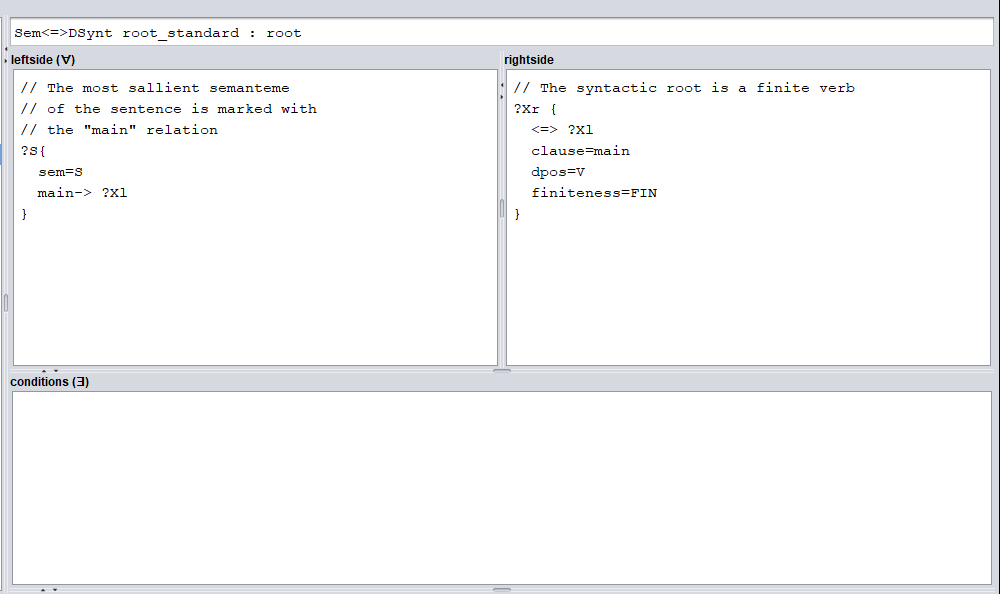
\includegraphics[width=1\textwidth, trim = {0cm 0cm 0cm 0cm},clip]{ch3/figs/grammaire.png}
	\caption{Règle créant la racine syntaxique}
	\label{fig:root}
\end{figure}

%%%%%%%%%%%%%%%%%%%%%%%%%%%%%%%%%%%%%%%%%%%%%%%%
% ---------G R A P H E S ------------------
%%%%%%%%%%%%%%%%%%%%%%%%%%%%%%%%%%%%%%%%%%%%%%%%

\subsubsection{Graphes}\label{entree-sortie}

Maitenant que nous avons fait un survol des dictionnaires et des modules de grammaires, il ne nous reste qu'à présenter les graphes. Dans un premier temps nous présenterons brièvement à quoi ressemble la construction d'un graphe en input. Puis nous montrerons à quoi ressemble les graphes en output.

L'input du réalisateur GenDR est un graphe sémantique \citep{mel2012semantics}\FL{\bf **** check ta biblio **** Daniel: le caractère spécial du c fonctionne pas avec Zotero, j'vais tenter de trouver une solution} où les prédicats sont liés à leurs arguments par des relations numérotées qui indiquent la position logique de l'argument. La figure~\ref{fig:debt} montre comment on construit un graphe sémantique dans MATE.

\begin{minipage}{\linewidth}
\begin{lstlisting}[language=XML, caption = Input sémantique, label=fig:debt]
structure Sem debt {
  S {
    owe {
    tense=PRES
    1-> Paul {class=proper_noun}
    2-> "\$500K" {class=amount}
    3-> bank {number=SG definiteness=DEF}}
    main-> owe } }
\end{lstlisting}
\end{minipage}

Toutefois, MATE offre aussi une version graphique pour encoder et visualiser le graphe sémantique (voir la figure \ref{fig:graphesem}).

\begin{figure}[htb]
	\centering
	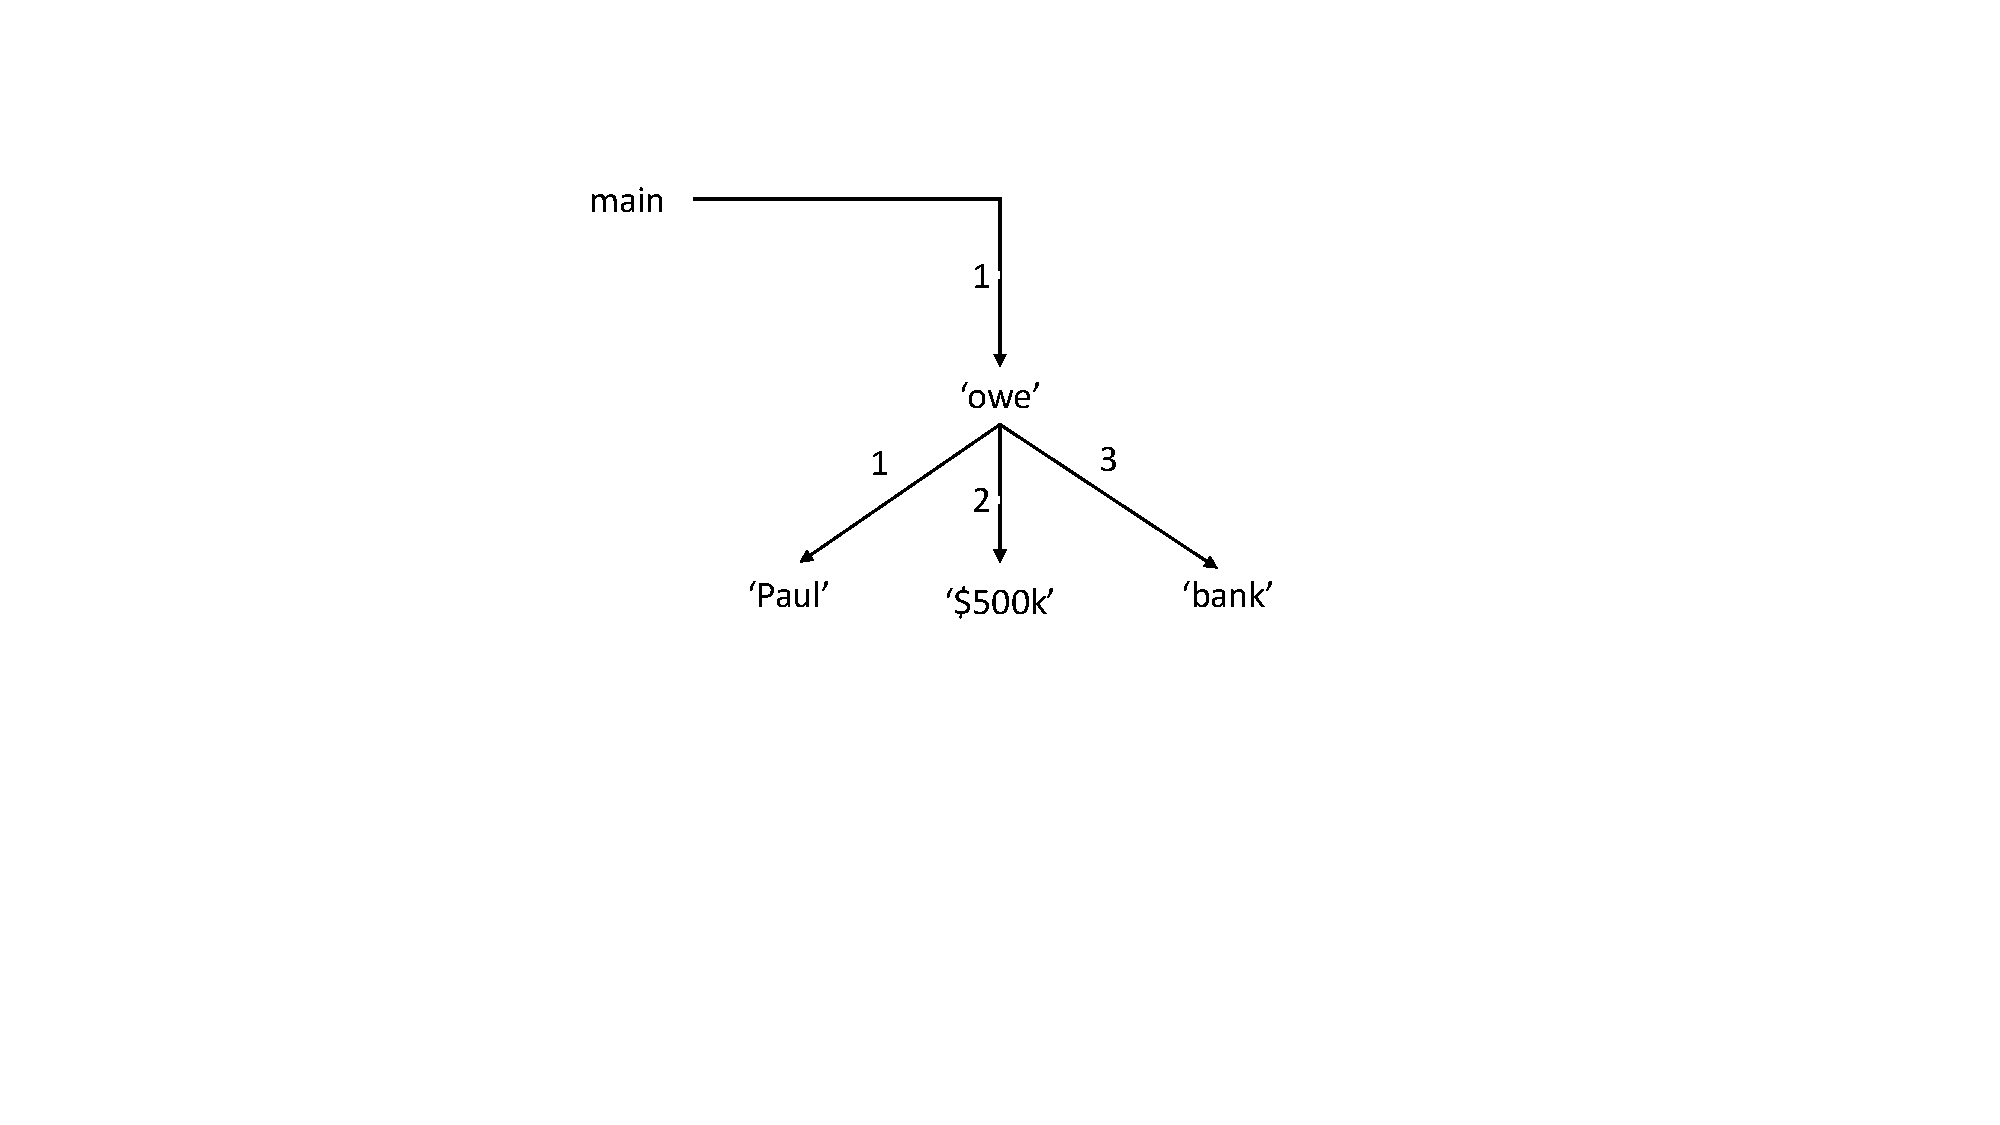
\includegraphics[width=1\textwidth, trim = {0cm 7cm 0cm 3cm},clip]{ch3/figs/owe_sem.pdf}
	\caption{Graphe sémantique en visuel}
	\label{fig:graphesem}
\end{figure}


La section graphe de GenDR nous permet de construire les structures sémantiques d'input et de visualiser les transductions de graphes. Pour l'input donné en \ref{input}, GenDR réalise six structures syntaxiques de surface. Celles-ci peuvent être visualisées dans MATE grâce au module de graphes. La figure \ref{fig:realsurfex} est un exemple d'output visuel que fournirait MATE. 

\begin{figure}[htb]
	\centering
	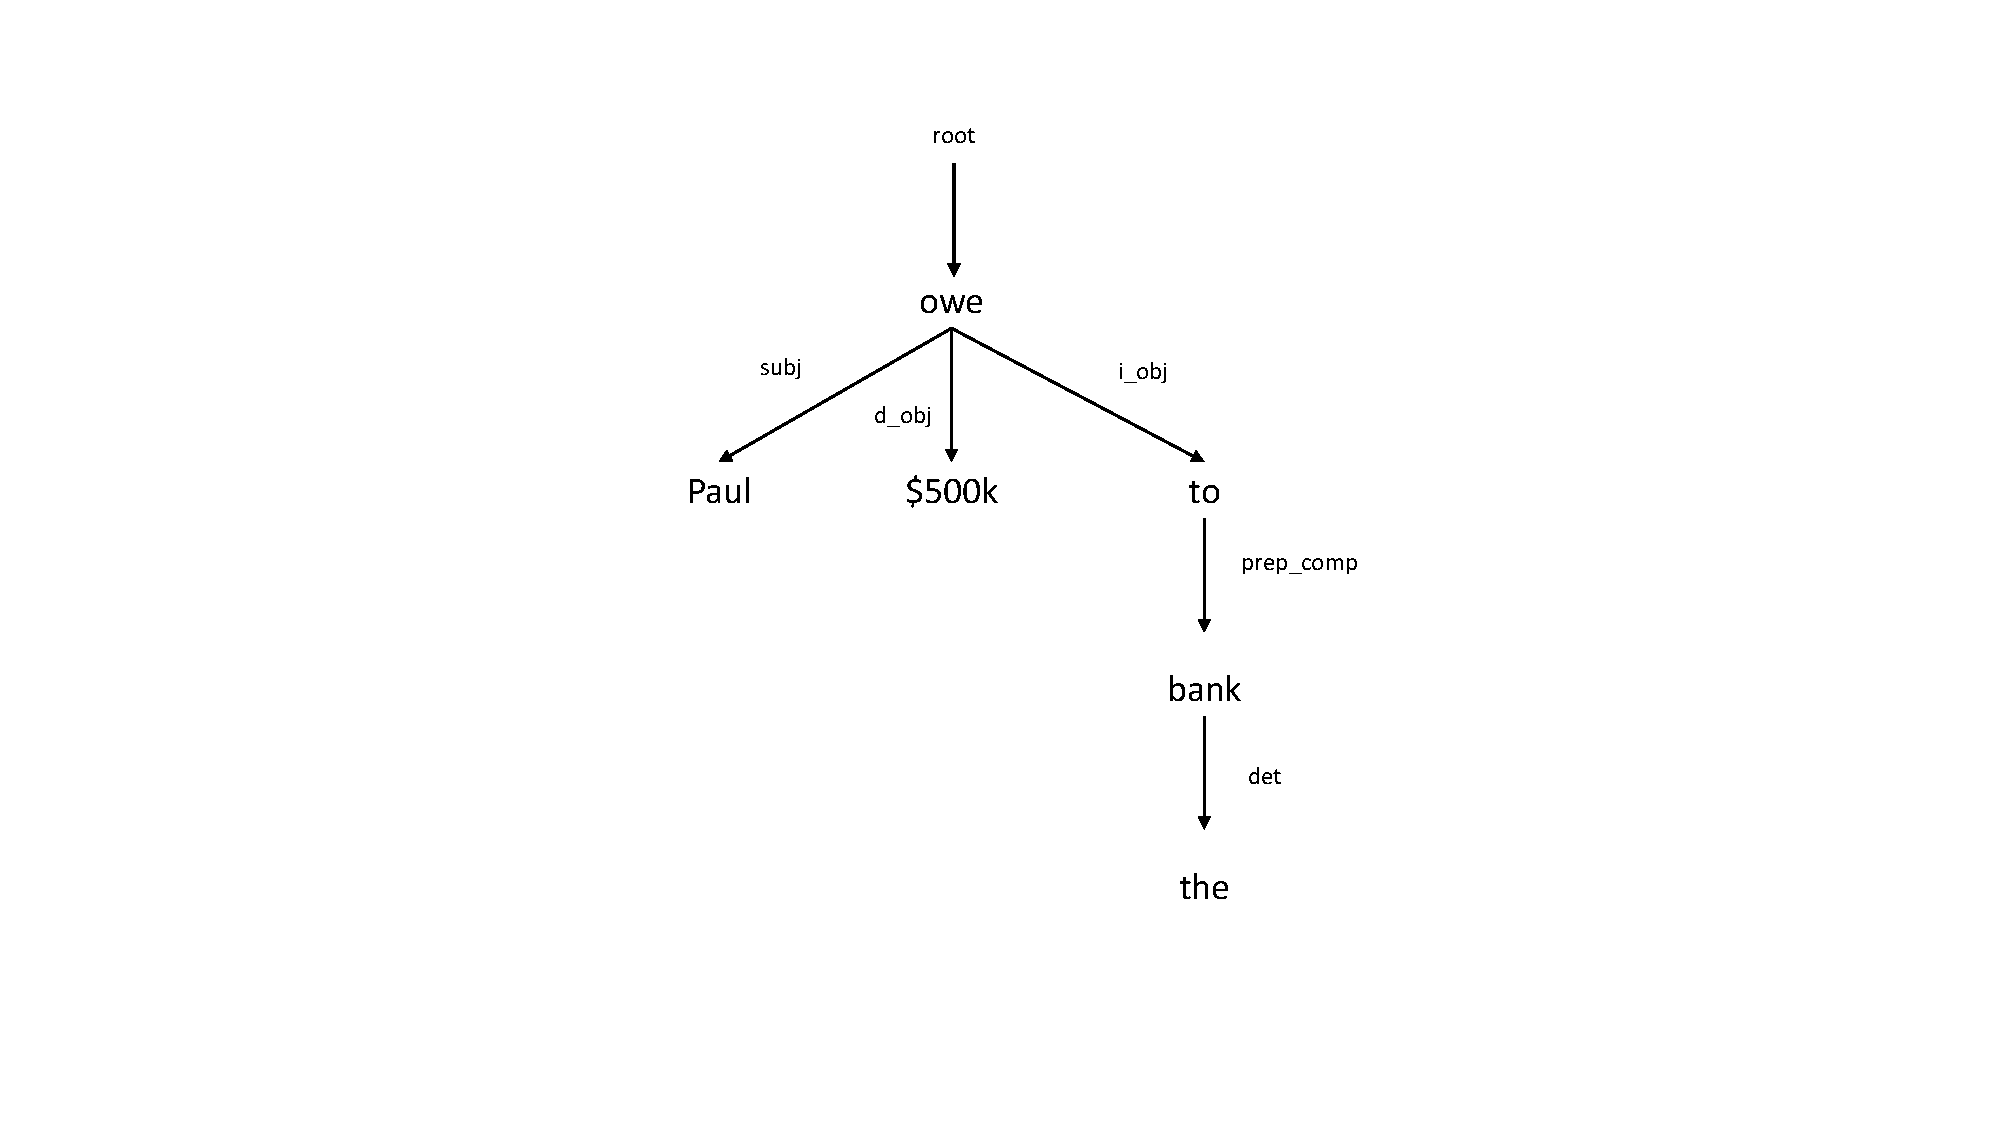
\includegraphics[width=1\textwidth, trim = {0cm 3cm 0cm 2cm},clip]{ch3/figs/realsurfex.pdf}
	\caption{Réalisation de surface}
	\label{fig:realsurfex}
\end{figure}

Toutefois, les modules de règles et de dictionnaires permettent en réalité de réaliser de six arbres syntaxiques superficiels (grâce aux mécanismes de paraphrasage). Nous les présentons à la figure \ref{fig:6realsurf}. Dans cette figure, les arbres de dépendances ont été linéarisés pour faciliter la compréhension du lecteur. Dans les faits, les arbres générés en output ne sont pas linéarisés et ils ressemblent à ceux de la figure \ref{fig:realsurfex}.

\begin{figure}[htb]
	\centering
	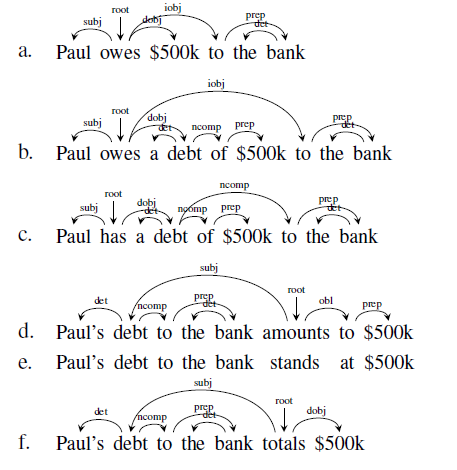
\includegraphics[width=0.5\textwidth, trim = {0cm 0cm 0cm 0cm},clip]{ch3/figs/exemples_real.png}
	\caption{Six réalisations syntaxiques de surface \citep{lareau18}}
	\label{fig:6realsurf}
\end{figure}
\FL{évite les captures d'écran si tu peux. Daniel: Oui, c'est temporaire, je vais tout' les refaire en pdf quand le texte sera prêt}

Si on souhaite une réalisation linéarisée et fléchie,  il faut utiliser un réalisateur de surface. C'est exactement dans ces contextes, que les réalisateurs de surface entrent en jeu \citep{DaoustJSREALTextRealizer2015, MolinsJSrealBBilingualText2015, GattSimpleNLGRealisationEngine2009, MilleSharedTaskProposal2017a,BelzFirstSurfaceRealisation2011}.

%%%%%%%%%%%%%%%%%%%%%%%%%%%%%%%%%%%%%%%%%%%%%%%%%%%%%%%%%%%%%%%%%%%%%%%%%%%%%
% --------- I N T E R F A C E   S É M A N T I Q U E- S Y N T A X E ---------
%%%%%%%%%%%%%%%%%%%%%%%%%%%%%%%%%%%%%%%%%%%%%%%%%%%%%%%%%%%%%%%%%%%%%%%%%%%%%

\section{Interface sémantique-syntaxe en TST}\label{sec:semsynt}

Dans la présente section, nous décrirons l'interface sémantique-syntaxe dans le cadre de la \ac{TST}. Plus précisément, nous expliquerons deux processus nécessaires au passage de la sémantique à la syntaxe: l'arborisation et la lexicalisation. Pour mieux comprendre où se situent ces procédés dans la modélisation du langage, nous ferons un très bref retour sur les fondements du cadre théorique que nous utilisons. 

La \ac{TST} vise la modélisation formelle de la correspondance entre les \emph{Sens} et les \emph{Textes} \citep{PolgueretheorieSensTexte1998, MelcukVerslinguistiqueSensTexte1997, DBLP:conf/coling/JolkovskyM67}. La figure \ref{fig:modeletst} (qui est issue de\cite{PolgueretheorieSensTexte1998}) présente comment fonctionnent ces modèles qui sont des machines virtuelles prenant en entrée des représentations sémantiques d'énoncés pour générer du texte. Celui-ci s'exprime par un ensemble de paraphrase exprimant le \emph{Sens} donné en input.

\begin{figure}[htb]
	\centering
	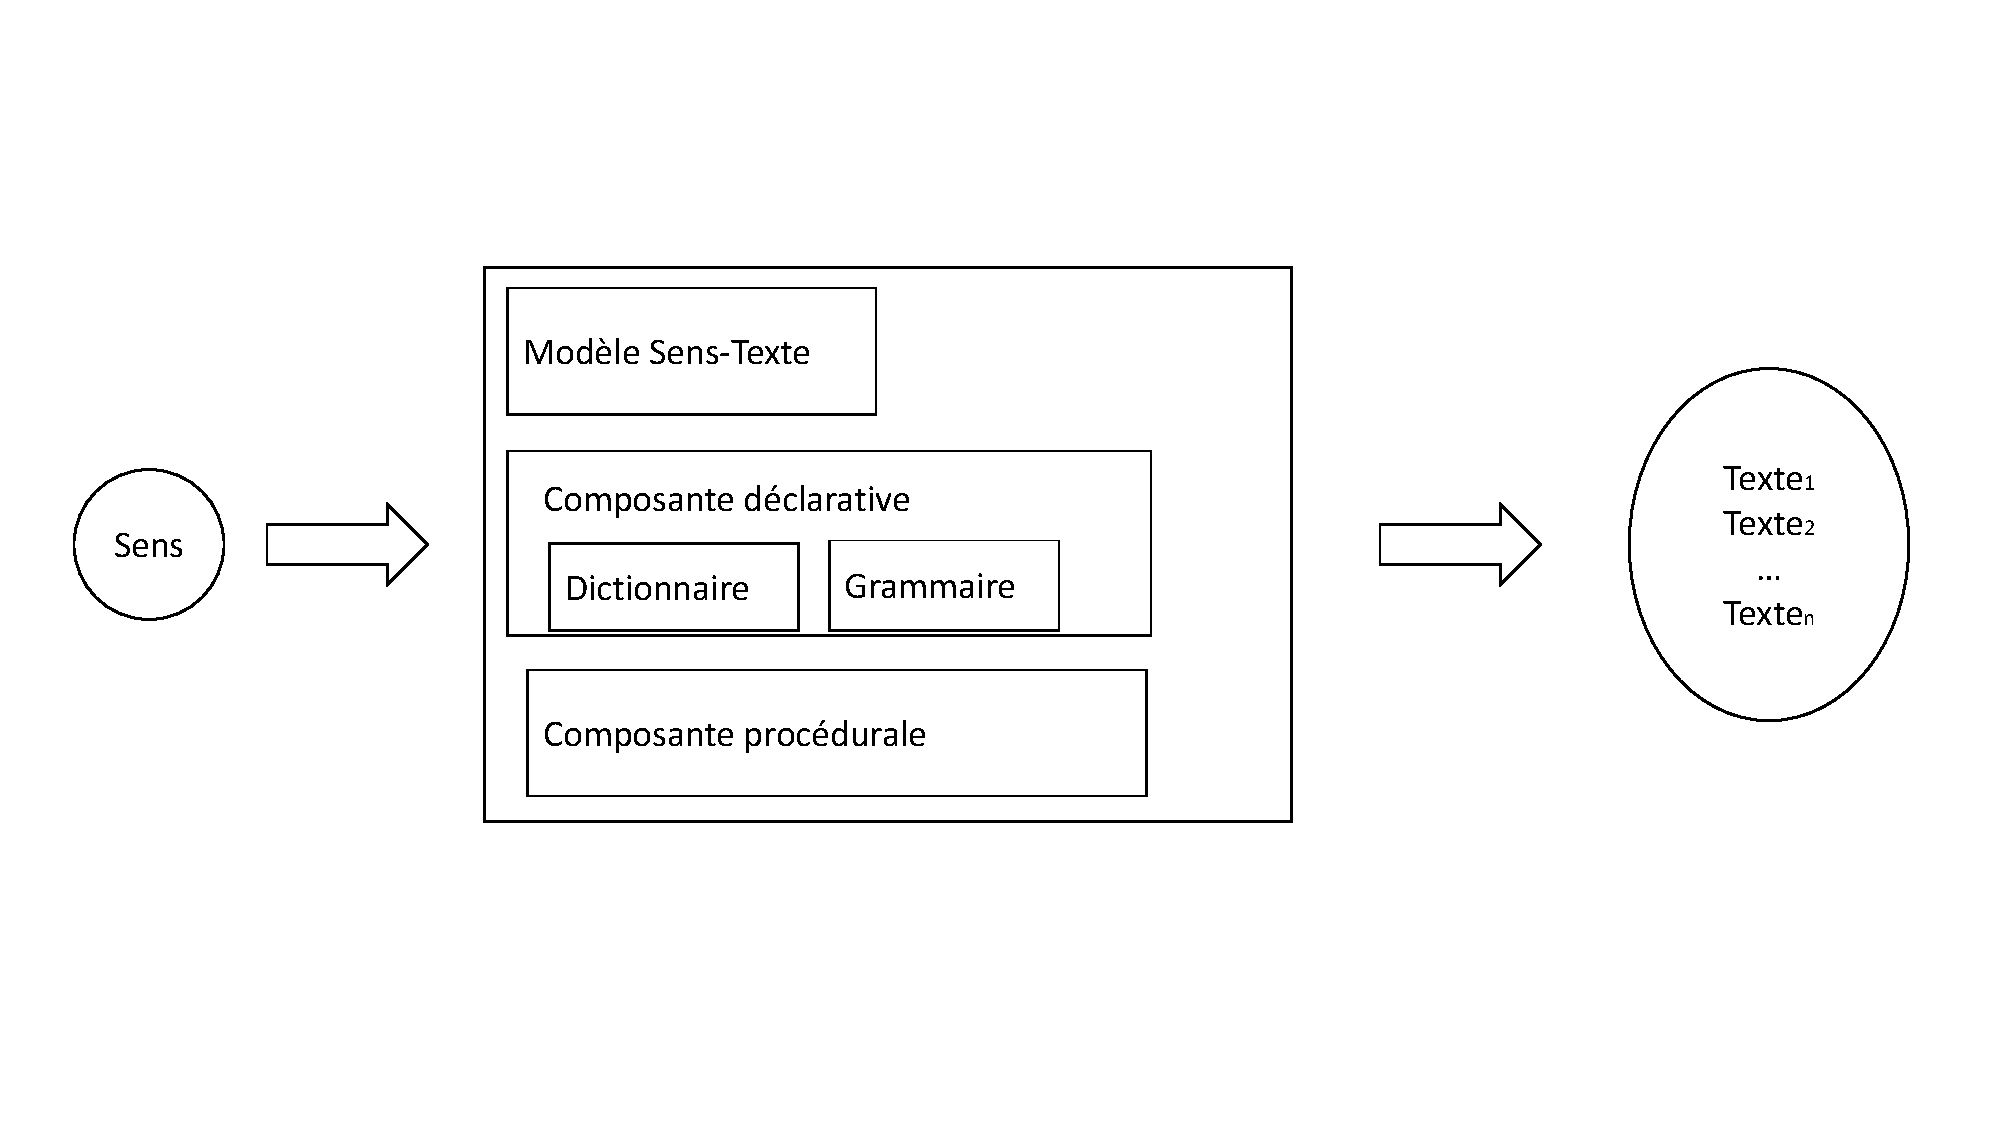
\includegraphics[width=1\textwidth, trim = {0cm 4cm 0cm 4cm},clip]{ch3/figs/polguere1.pdf}
	\caption{Structure d'un modèle Sens-Texte \citep{PolgueretheorieSensTexte1998}}
	\label{fig:modeletst}
\end{figure}

Pour se rendre au \emph{Texte} final, le \emph{Sens} traverse de nombreux niveaux de représentations. La figure \ref{fig:processustst} illustre les transformations que l'input doit subit succesivement. La figure illsutre aussi parallèlement le formalisme utilisé pour modéliser les représentations diverses.

\begin{figure}[htb]
	\centering
	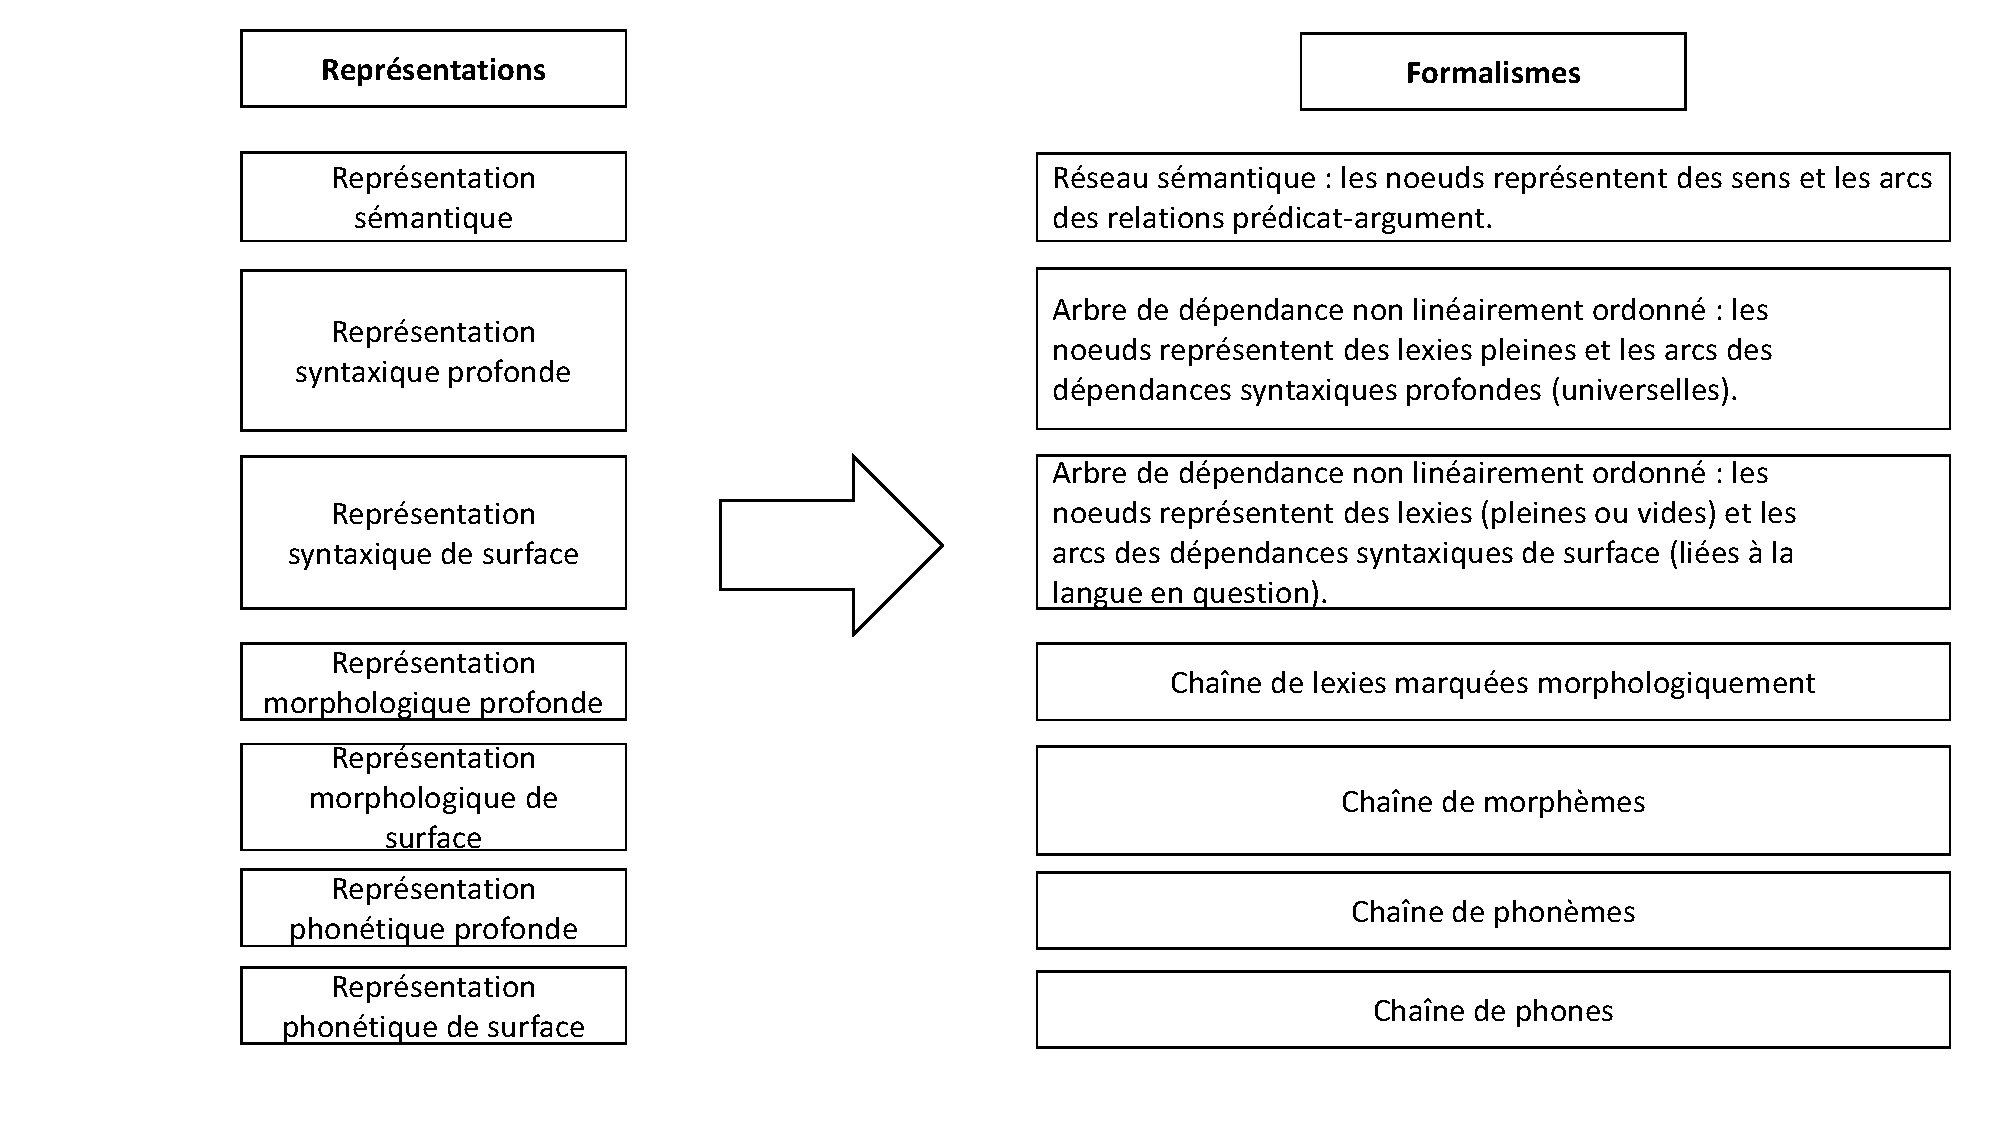
\includegraphics[width=1\textwidth, trim = {0cm 0cm 0cm 0cm},clip]{ch3/figs/polguere2.pdf}
	\caption{Processus d'un modèle Sens-Texte \citep{PolgueretheorieSensTexte1998}}
	\label{fig:processustst}
\end{figure}

%%%%%%%%%%%%%%%%%%%%%%%%%%%%%%%%%%%%%%%%%%%%
% --------- A R B O R I S A T I O N  ------
%%%%%%%%%%%%%%%%%%%%%%%%%%%%%%%%%%%%%%%%%%%

\subsection{Arborisation}\label{sec:arbo}

Tel que nous l'avons mentionné, le réalisateur GenDR modélise spécifiquement trois niveaux de représentations (\ac{RSem}-\ac{RSyntP}-\ac{RSyntS}). L'arborisation, qui est le processus de création de la syntaxe profonde à partir d'une structure sémantique, se situe dans ces trois niveaux. Nous la décrirons à la fois d'un point de vue théorique et comment cela se traduit dans le cadre de notre projet.

Selon la \ac{TST}, la structure syntaxique d'un énoncé représente l'ensemble des liens de dependances fonctionnelles qui existent entre les unités lexicales de cet énoncé \citep{melcuk1988}. On représente formellement ces structures syntaxiques par des arbres de dépendances. Cette approche syntaxique provient de \cite{TesniereElementssyntaxestructurale1965} qui est le premier à l'avoir théorisée. Formellement, le passage de la \ac{RSem} à la \ac{RSyntP} se nomme l'arborisation parce qu'on cherche à arboriser la structure sémantique pour qu'il en résulte un arbre de dépendance profond grâce à l'application de règles de correspondance sémantiques. Nous reprendrons donc la description que \cite{lareau18} fait de l'arborisation dans GenDR. D'ailleurs, l'arbre syntaxique profond est construit avec un algorithme \emph{top-down} qui ressemble énormément à celui qu'utilise FORGe puisque ces deux réalisateurs profonds l'ont hérité de MARQUIS, qui est inspiré de \cite{PolguereStructurationmisejeu1990}.

Bref, dans GenDR, l'arborisation se divise en trois étapes \citep{lareau18}.

\begin{enumerate}
  \item Création de la racine.
  La première règle appliquée est \emph{root\_standard}, elle construit la racine de l'arbre syntaxique à partir du \ac{ND} de la structure sémantique. À cette étape, la racine n'est pas étiquetée par un lexème encore (le n\oe{}ud est vide), mais des contraintes lui sont imposées. La détermination de la racine correspond au processus de hiérarchisation de \cite{PolguereStructurationmisejeu1990} car la racine est le n\oe{}ud dominant (au sommet de la hiérarchie) tous les autres.

  \item Lexicalisation de la racine.
  Une fois que la racine a été créée et contrainte, on applique une règle de lexicalisation (appellée \emph{lex\_standard}) qui permet au système de fouiller dans les dictionnaires pour trouver un lexème qui correspondra au sens demandé tout en respectant les contraintes imposées. Ainsi, il faut que le lexème sélectionné corresponde au \ac{ND} en sémantique et qu'il possède une \ac{dpos} de type verbale généralement. Effectivement, les langues européennes imposent souvent cette contrainte sur la racine puisque ce sont essentiellement les verbes qui contrôlent les énoncés.

  \item Application des règles actancielles.
  Une fois que le n\oe{}ud racine est lexicalisé, GenDR regarde dans le \ac{GP} de la racine pour savoir comment effectuer le passage des arcs sémantiques aux arcs syntaxiques. Autrement dit, on ajoute les arcs dépendant de la racine qui correspondent aux arguments liés au \ac{ND} dans la \ac{RSem}. Comme Polguère le dit:
\begin{quote}
chaque arc est considéré successivement dans l'ordre du parcours, puis est traduit en une micro-structure syntaxique profonde grâce aux règles de correspondance sémantique de la grammaire.
\end{quote}
\vspace{-\baselineskip}
\hfill
\cite[p.~273]{PolguereStructurationmisejeu1990}

Les micro-structures syntaxiques correspondent aux branches de l'arbre et à leurs noeuds qui se font, à leur tour, imposer des contraintes par le \ac{GP} du noeud qui les gouverne (la racine). C'est ainsi qu'on retourne à la seconde étape pour lexicaliser ces n\oe{}uds. Puis cycliquement, nous retournons à la troisième étape puisque de nouveaux n\oe{}uds lexicalisés amènent leur patron de régime avec eux. Et ce jusqu'à ce que le graphe sémantique soit complètement réalisé en surface profonde.
\end{enumerate} 

Une fois que l'arborisation est complétée, le système doit effectuer l'arborisation de surface ce qui implique les opérations suivantes. D'abord, faire le calcul des relations syntaxiques de surface (la relation I deviendra sujet, la relation II deviendra complément d'objet direct, etc.) et incorporer les lexies vides (prépositions, déterminants, etc.). Cela est effectué grâce aux règles de correspondances profondes et aux informations contenues dans les \ac{GP} des entrées lexicales.

%%%%%%%%%%%%%%%%%%%%%%%%%%%%%%%%%%%%%%%%%%%%%%%%%%%%%
% ---------  L E X I C A L I S A T I O N  ------
%%%%%%%%%%%%%%%%%%%%%%%%%%%%%%%%%%%%%%%%%%%%%%%%%%%%
\subsection{Lexicalisation}

Le processus de lexicalisation est dispersée sur plusieurs niveaux de représentation (\ac{RSem}, \ac{RSyntP}, \ac{RSyntS}) formant deux interface (\ac{RSem}-\ac{RSyntP}, \ac{RSyntP}-\ac{RSyntS}) \citep{PolguerePourmodelestratifie}. La première interface modélise la lexicalisation profonde qui consiste à assure la correspondance entre une unité sémantique dont les traits (de type definiteness ou tense, voir figure x) sont remplacés par des traits grammaticaux et dont le sens est remplacé par une (ou des) unité(s) lexicale(s) profonde(s). Cette correspondance est explicité dans le dictionnaire d'un système \ac{TST}. S'ensuit la lexicalisation de surface qui consiste à introduire les mots fonctionnels (déterminants, auxiliaires, prépositions,etc.) et les lexies de surface (comme dans l'exemle que nous avons montré plus haut avec peur bleu où bleu serait réalisée en surface). \draft{Daniel: Je n'ai pas trouvé la citation sur la lexicalisation de Wanner dont tu parlais (dans le mémoire de Flo)}

Afin d'illustrer le fonctionnement de la lexicalisation dans GenDR, nous repredrons la description de \cite{lareau18}.

\textbf{Les lexicalisations simples}
sont traitées par la règle \emph{lexicalization\_standard} qui prend une unité sémantique donnée dans un graphe d'input et récupères dans le \emph{semanticon} les correspondances lexicales de ce sémantème (tel que démontré en \ref{fig:semanticon}). S'ensuit la sélection de l'unité lexicale: GenDR s'assure que \ac{DPOS} de la (ou les) lexie(s) correspond à celle qui est demandée par le n\oe{}ud contraint dans l'arbre syntaxique profond en construction. Le no\oe{}ud en question de l'arbre syntaxique profond sera désormais lexicalisé. D'ailleurs, c'est ce mécanisme qui permet le paraphrasage dans notre système, puisqu'il crée autant d'arbres syntaxiques profonds qu'il y a de lexies possibles pour un n\oe{}ud donné.

\textbf{Les lexicalisations de classes}
comme les nombres, les montants, les noms propres ou les acronymes sont prises en charge par la règle \emph{lex\_class}. Sont but est de lexicaliser les unités sémantiques que nous ne voulons pas dans nos dictionnaires sémantiques et lexicaux parce qu'elles sont trop nombreuses et leur comportement est prévisible. Pour déclencher l'application de cette règle, on précise dans la structure d'input à quelle classe le sémantème appartient. Celle-ci contient les informations nécessaires à la lexicalisation d'un n\oe{}ud donné (la \ac{dpos}, la \ac{spos}, le nombre, l'invariabilité, la comptabilité,etc.)

\textbf{La lexicalisation de secours} 
permet à GenDR de lexicaliser une unité sémantique ou lexicale dont il n'a pas les informations. Effectivement, comme le système possède les 1\,500 lexies les plus fréquentes de l'anglais, il est évident que certaines lexies ou sémantèmes manqueront à l'appel. Pour remédier à la situation, il y a d'abord un mécanisme qui vérifie si l'input existe sous la même forme dans le \emph{lexicon}. Si c'est le cas, alors le système réalisera le sémantème à l'aide de ce lexème. Cette particularité du système a pour conséquence qu'on n'a pas besoin d'inscrire le sémantème dans le \emph{semanticon} s'il n'y a qu'une seule lexicalisation possible de celui-ci (cela permet de sauver du temps). Cependant, si le sémantème ne figure pas dans le \emph{lexicon}, alors le système suppose que l'étiquette de l'unité sémantique est la même que l'unité lexicale, et s'il y a des contraintes sur le n\oe{}ud d'arrivée, alors le système supposera que l'unité lexicale ainsi créée satisfait les contraintes. Les lexèmes devinés seront mis en évidence dans la structure d'output afin qu'on ait une trace que le système a fait une tentative.

\textbf{La lexicalisation grammaticale}
introduit des lexèmes fonctionnels (dét., aux., etc.) et prend place au entre la \ac{RSyntP}-\ac{RSyntS}. Ce type de règle est déclenché par la présence de sens grammaticaux dans les structures d'input comme la définitude ou le temps (voir la figure \ref{fig:debt}). Ces lexèmes existent en syntaxe profonde, mais sous forme de traits sur les n\oe{}uds lexicaux. Comme ces lexies appartiennent à une classe fermée et qu'ils sont peu nombreux (en plus d'être spécifiques à une langue), ils sont lexicalisés par une règle spéciale qui sait comment réaliser les traits grammaticaux. Puis, il y a aussi des règles de lexicalisation grammaticales qui s'occupent des lexèmes imposés en surface par les régimes de certaines lexies (comme les prépositions). Ce type de lexème est introduit en syntaxe comme un n\oe{}ud supplémentaire entre un gouverneur et son actant. Ils sont donc encodés dans le \ac{GP} du gouverneur. \draft{pas clair}

%%%%%%%%%%%%%%%%%%%%%%%%%%%%%%%%%%%%%
% --------- E X E M P L E ---------
%%%%%%%%%%%%%%%%%%%%%%%%%%%%%%%%%%%%%

\section{Exemple}\label{sec:exemple}

Pour illustrer le fonctionnement des règles et des dictionnaires que nous venons de présenter, nous décortiquerons la réalisation profonde de l'exemple vu à la figure~\ref{fig:debt}.

\subsection{Arborisation profonde}

Cette section illustre les étapes successives qui ont permis à GenDR de passer de la \ac{RSem} à la \ac{RSyntP}.

\subsubsection{Application de la règle \emph{root\_standard}}
La règle crée un n\oe{}ud vide qui sera la racine de l'arbre à construire et qui se fait imposer les contraintes suivantes: \texttt{dpos=V} (la racine doit être un verbe) et \texttt{finiteness=FIN} (tensé). La figure \ref{fig:rootstand} illustre la création du n\oe{}ud non-étiqueté.
\begin{figure}[htb]
	\centering
	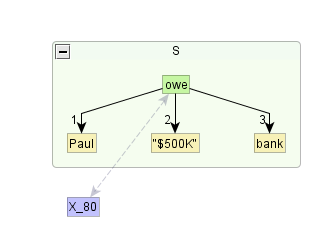
\includegraphics[width=0.6\textwidth, trim = {1cm 0.5cm 0cm 1cm},clip]{ch3/figs/inspecteur_root.png}
	\vspace{-0.5cm}
	\caption{Application de \emph{root\_standard}}
	\label{fig:rootstand}
\end{figure}

\subsubsection{Application de la règle \emph{lex\_standard}}
La racine vide déclenchera l'application d'une règle de lexicalisation, c'est pourquoi GenDR fouillera dans le dictionnaire à la recherche des lexèmes représentant le sémantème \sem{owe} \lstinline! owe { lex=owe lex=debt}!. GenDR peut ainsi lexicaliser la racine en choisissant \lex{debt} ce qui entraînera l'application d'une fonction lexicale permettant de réaliser un verbe support à la racine (ce qui satisfait la contrainte \texttt{dpos=V}). Il s'agit d'une lexicalisation complexe, donc nous renvoyons le lecteur à \cite{lambrey15,LambreyImplementationcollocationspour2017,lareau18} pour nous concentrer sur la lexicalisation simple effectuée grâe au lexème \lex{owe}.

\begin{figure}[htb]
	\centering
	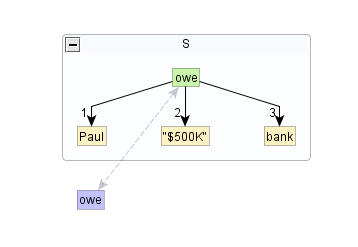
\includegraphics[width=0.7\textwidth, trim = {0cm 0.7cm 0cm 0.9cm},clip]{ch3/figs/lex_standard_root.png}
		\vspace{-0.5cm}
	\caption{Application de lex\_standard}
	\label{fig:lexstand1}
\end{figure}

\subsubsection{Application de la règle \emph{actant\_gp}}
Une fois que la racine est pourvue d'un lexème, l'application de la règle \emph{actant\_gp} est déclenchée. Celle-ci traduit les relations sémantique prédicat-argument de \sem{owe} en arcs syntaxiques profonds. La correspondance est confirmée par les informations sur la diathèse encodée dans le régime de la lexie \lex{owe}. Comme le prédicat lie trois actants sémantiques, alors la règle s'applique trois fois pour chaque relation. Ensuite, les n\oe{}uds au bout des arcs syntaxiques seront contraints en fonction des restrictions prévues par le \ac{GP} de \lex{owe}. Ce mécanisme assure la grammaticalité de la construction de l'arbre. Pour cet exemple, le \ac{GP} de \lex{owe} permet à son deuxième actant syntaxique d'être soit un nom ou un nombre (la figure \ref{fig:dictio} illustre le régime du verbe).

\begin{figure}[htb]
	\centering
	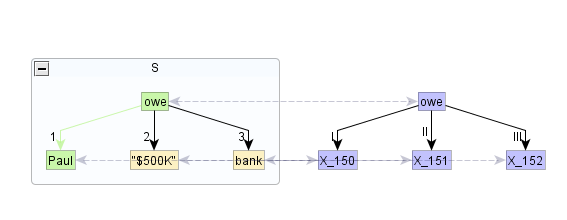
\includegraphics[width=1\textwidth, trim = {0cm 8mm 0cm 15mm},clip]{ch3/figs/actant_gp1.png}
	\caption{Application de actant\_gp}
	\label{fig:actantgp}
\end{figure}

\subsubsection{Application des règles \emph{lex\_class} et \emph{lex\_standard}}

L'étape précédente a généré des arcs contraints en partance de la racine. Les n\oe{}uds de ces arcs devront donc être lexicalisé afin de poursuivre l'arborisation. GenDR répètera opèrera deux règles de lexicalisation pour ce faire afin de réaliser les lexèmes correspondant à \sem{Paul}, \sem{bank} et \sem{\$500}. Les règles (\emph{lex\_class}) et (\emph{lex\_standard}) seront utilisés puisque \sem{Paul} et \sem{\$500} affichaient les traits respectifs \texttt{class=proper\_noun} et \texttt{class=amount} dans l'input sémantique. La règle fait en sorte que GenDR passe directement au \emph{lexicon}, puisque les sens ne sont pas décrits dans le \emph{semanticon}. L'étiquette du n\oe{}ud sémantique est directement copiée en syntaxe puis GenDR s'assure finalement que les traits de \lex{Paul} et \lex{\$500} respectent les contraintes des n\oe{}uds générés par la règle précédente.

\begin{figure}[htb]
	\centering
	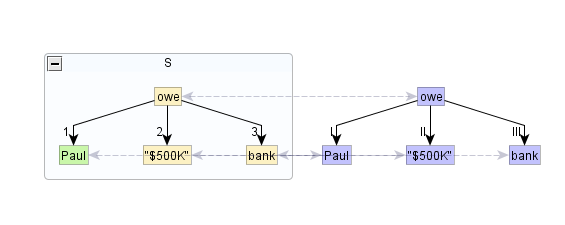
\includegraphics[width=1\textwidth, trim = {0cm 8mm 0cm 10mm},clip]{ch3/figs/lex_standard2.png}
	\caption{Application des règles de lexicalisation}
	\label{fig:lexstand2}
\end{figure}

\FL{trim les figures}

\subsection{Arborisation de surface}

\subsubsection{Application des règles de lexicalisation de surface}
On va chercher les lexicalisations de surface de chacune des unités lexicales avec les règles \emph{lex\_class} (qui s'occupe des lexèmes comme \lex{Paul}) et \emph{lex\_lu}. Il y en a deux, car il faut une règle spécifique pour les lexèmes appertenant à des classes puisque leurs traits de surface ne sont pas encodé dans leurs entrées lexicale, mais dans la classe qui leur est assignée.

\begin{figure}[htb]
	\centering
	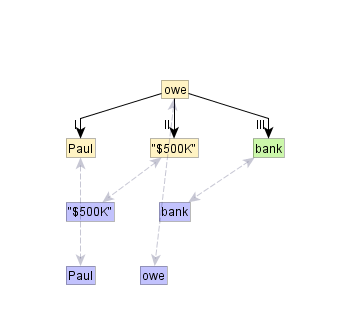
\includegraphics[width=0.6\textwidth, trim = {0cm 13mm 0cm 2cm},clip]{ch3/figs/rsyntslexicalisation1.png}
	\caption{Application des règles de lexicalisation de surface}
	\label{fig:lexsurf}
\end{figure}

\subsubsection{Application des règles actancielles de surface}
Concrètement, ces règles remplacent les étiquettes des arcs de l'arborisation profonde (I, II, III,...) par des étiquettes de surface (sujet, objet direct, objet indirect,...) qui sont encodées dans le \ac{gp} du verbe qui gouverne les actants syntaxiques. Ainsi, la relation subjectale est réalisée par la règle \emph{actant\_subj}. Qui réalise la relation entre le sujet et le verbe. Cette information est encodée dans le gp du verbe \lex{owe} qui hérite des traits de la classe verb\_dit. Celle-ci hérite des traits de la classe verb\_dt qui hérite des traits de la classe verb. C'est dans celle-ci que se trouve l'information nécessaire à l'application de la règle \lstinline!gp = { I = { dpos = N rel = subjective } } !. Ainsi, on voit encore comment le dictionnaire et les règles sont inter-reliés. Pour que la règle actant\_subj s'applique au sujet de la structure, elle va regarder dans la dictionnaire à quel actant syntaxique elle doit faire le lien. Elle ne prend que l'actant syntaxique qui précise la relation subjective.

Les mêmes phénomènes s'appliquent ensuite pour les règles \emph{actant\_dir} et \emph{actant\_prep}. Toutefois, la règle \emph{actant\_prep} diffère des deux autres règles actancielles car elle crée un n\oe{}ud intermédiaire en syntaxe de surface pour accueillir le lexème fonctionnel \lex{to} qui est nécessaire à la bonne formation de la phrase. La nature de la préposition est encodée dans le gp du verbe ainsi \lstinline! gp = {III = { dpos = N  rel = indir_objective  prep = to }  }!.

\subsubsection{Application de la règle des déterminants}

La règle \emph{det\_def} ajoute les déterminants aux lexèmes en fonction de leur définitude. Parmi les règles que nous avons présenté, c'est la seule règle de GenDR qui est propre à l'anglais. Elle lexicalise \lex{the} puisque l'unité sémantique \sem{bank} était marquée par le trait défini dans la structure d'input.

La figure \ref{fig:syntsurf} démontre l'application simultanée des règles actancielles et de la règle des déterminants.

\begin{figure}[htb]
	\centering
	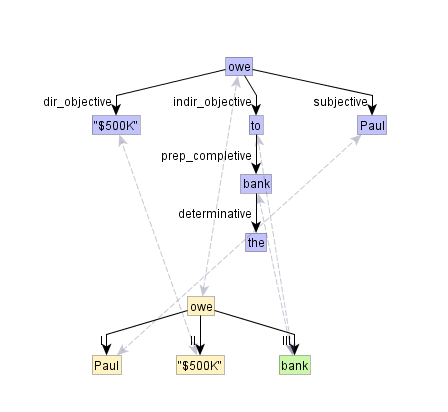
\includegraphics[width=0.7\textwidth, trim = {0cm 8mm 0cm 15mm},clip]{ch3/figs/rsynts_syntactisation.png}
	\caption{Application de subj,dir,prep et det}
	\label{fig:syntsurf}
\end{figure}

%%%%%%%%%%%%%%%%%%%%%%%%%%%%%%%%%%%%%%%%%%%%%%%%
% --------- P R O B L É M A T I Q U E ---------
%%%%%%%%%%%%%%%%%%%%%%%%%%%%%%%%%%%%%%%%%%%%%%%%

\section{Problématique}\label{sec:problema}

La démonstration précédente montre que GenDR modélise avec aisance des phénomènes linguistiques profonds. Toutefois, le dictionnaire lexical de ce système ne couvre que les 1\,500 lexies les plus fréquentes (en anglais et en français). Parmi celles-ci, 500 sont des verbes. Cela est non-négligeable, certes, mais il est clair que GenDR gagnerait en couverture linguistique s'il se dotait d'une ressource lexicale lui permettant de traiter une plus grande quantité de verbes. Pourquoi les verbes en particulier ? Parce qu'ils sont très riches en paraphrasage et car ils démontrent des irrégularités. Effectivement, on peut difficilement prédire le comportement d'un verbe, c'est pourquoi il faut encoder ces comportements dans des dictionnaires. De plus, les verbes contrôlent la majorité des énoncés. Donc, en détenant les propriétés lexicales de combinatoire des verbes, on peut couvrir une immense partie du langage.

\begin{quote}
In particular, since verbs often convey the main idea of a sentence, such a resource must represent verb meanings. These require a particularly precise and well deffined representation that captures both their predicate-argument structure as well as their semantic content.
\end{quote}
\vspace{-\baselineskip}
\hfill
\cite{SchulerVerbnetBroadcoverageComprehensive2005}

Nous sommes en accord avec cette déclaration, tout comme \cite{Korhonenlargesubcategorizationlexicon2006} et \cite{MESSIANT08.142} qui suggèrent aussi que la modélisation informatique des langues naturelles passe par des ressources lexicales décrivant les comportements syntaxiques des lexèmes.  C'est la raison d'être de ce mémoire, car notre objectif est d'intégrer au réalisateur profond GenDR  un dictionnaire verbal doté des \acp{GP} de ceux-ci.

\section{Patrons de régime}\label{sec:gp}

Ce qu'on appelle \ac{GP} a aussi plusieurs noms dans d'autres cadres théoriques (cadre valenciel, valence, cadre de sous-catégorisation, cadre syntaxique, schéma de régime, etc.), mais c'est le nom qu'on emploiera dans ce mémoire. Les \acp{GP} décrivent les cooccurrences syntaxiques des unités lexicales \citep{MilicevicSchemaregimepont2009} avec leurs actants (les sujets et objets des verbes, les compléments du nom,etc.). Les patrons de régime d'une lexie correspondent à l'ensemble des constructions syntaxiques dont la lexie est la gouverneure. Les actants syntaxiques en sont ses dépendants. On les encode dans un dictionnaire car les patrons de régime des lexies ne sont généralement pas prévisibles. Effectivement, on ne peut pas prédire les \acp{GP} des unités lexicales d'une langue. D'ailleurs, même des verbes sémantiquement proches ne possèderont pas nécessairement les mêmes constructions syntaxiques ex de Milicevic p. 95( se souvenir de X , mais se rappeler X ). Le nombre d'actant n'est pas prévisible non plus en regardant l'unité lexicale à partir de son sens. 

Puisque les arguments sélectionnés par une lexie sont généralement idiosyncratiques, on encode ces comportements syntaxiques dans des dictionnaires.

les GP encodent la diathèse (correspondance entre les actants sémantiques d'une lexie et ses actants syntaxiques profonds) et la réalisation des actants (I à sujet II objet direct, indirect, ou oblique). La diathèse peut soit être triviale (1 pour I, 2 pour II, etc.) ou pas (1 -II et 2-I)

Le patron de régime d'une lexie encode les correspondances entre ses actants (au niveau sémantique, syntaxique profond et syntaxique de surface), les moyens morpho-syntaxiques d'expressions des actants et les restriction sur les actants.

Plus tôt dans le chapitre nous avions parlé de l'interface sémantique-syntaxe et de l'importance des règles sémantiques qui font la transition entre Rsem et RSyntP. Le rôle le plus important du GP est de fournir l'information nécessaire au passage de la sem à la synt lors des opérations de lexicalisation et d’arborisation. 

\begin{quote}
Comme le choix lexical détermine le choix des constructions syntaxiques possibles (la lexie sélectionnée « amène » avec elle son régime) et vice-versa (le choix d’une structure impose certains choix lexicaux), on peut dire que c’est le schéma de régime qui, au sein d’un MST, fait le pont entre le lexique et la grammaire.
\end{quote}
\vspace{-\baselineskip}
\hfill
\cite[p.~105]{MilicevicSchemaregimepont2009}

le logiciel MATE présente des limites d'encodage quant à la manière dont les gp sont encodés présentement dans GenDR. Pour un verbe donné, on ne peut pas avoir deux parties du discours différentes qui compétitionnent pour la même position syntaxique. Autrement dit, prenons le cas de X (exemple). Cela restreint le nombre de génération possible pour un verbe ou bien ça peuple inutilement le dictionnaire d'entrée verbale par partie du discours qu'il prend. Ce n'est pas une manière efficace d'encoder le langage. C'est là qu'un dictionnaire de patron de régime entre en ligne de compte. Et ça permet une grande couverture de la langue. Sans dictionnaire de patron de régime ni d'acquisition automatique de ceux-ci, il faut les encoder à la main un par un. Ce n'est pas une tâche rationnelle. C'est ainsi que plusieurs groupes de recherches ont voulu remédier à cette situation. Plusieurs s'entendent pour dire qu'un meilleur traitement du \ac{TAL} se fait grâce à des ressources lexicales riches. C'est pour cette raison que nous avons pensé implémenter un dictionnaire de verbe à GenDR pour le rendre plus performant. Nous nous sommes finalement retourner vers VerbNet, une ressource lexicale très riche.
\draft{tu devrais mieux expliquer le problème des GP multiples}
%!TEX root = ../memoire.tex

\chapter{Un dictionnaire de patrons de régime: VerbNet}

Avant de parler de VerbNet, nous expliquerons pourquoi nous l'avons choisi parmi tant de candidats possibles. Dans la section qui suit, nous ferons un bref survol de ces candidats. Nous avons analysé les composantes de: WordNet, FrameNet, XTAG, LCS, Comlex, Valex, LexSchem, VDE et le dicovalence. Parmi ces dictionnaires, il y en a qui traitent de d'autres parties du discours tandis que certains ne traitent uniquement que des verbes. Le Dicovalence est le seul dictionnaire francophone que nous avons analysé, les autres ont été programmés en anglais à la base.

\section{Dictionnaires verbaux concurrents}

\subsection{WordNet}
Wordnet \citep{Fellbaum1998} est une base de données lexicales traitant les verbes, noms, adjectifs et adverbes de la langue anglaise. Cette base de données s'organise en \emph{synset}: des ensembles de synonymes. Il ne s'agit pas nécessairement de synonymes exacts, mais plutôt d'un ensemble de lexies, d'une même partie du discours, unis par des traits conceptuo-sémantiques. Ces \emph{synset} sont associés à une définition et un exemple d'utilisation. WordNet est une base de données hiérarchisée. Elle est construite via des liens d'hyperonymie et d'hyponomie entre les \emph{synsets}. Les synsets sont répartis parmi les classes suivantes. S'il s'agit de verbes dénotant des actions ou des évènements, ils seront classés parmi: \emph{ motion, perception, contact, communication, competition, change, cognition, consumption, creation, emotion, perception, possession, bodily care and functions, social behavior and interactions}. S'il s'agit de verbes dénotant des états, on le retrouvera parmi les classes de type: \emph{resemble, belong, suffice}, ou des classes de type: \emph{want, fail, prevent, succeed}, ou de types aspectuels comme \emph{begin} \citep{Fellbaum1998}. À l'intérieur d'une entrée, on retrouve aussi des liens lexicaux: synonymes, antonymes, troponymes, implication et causation \citep{SchulerVerbnetBroadcoverageComprehensive2005}. Cela leur a permis de tisser une toile sémantique assez volumineuse.

À la base, WordNet a été conçu comme réseau lexical. Cela explique pourquoi il contient peu d'information syntaxique. La ressource fournit des définitions, des exemples et des \emph{synsets}, mais ne nous donne pas d'information sur la structure sémantique ou syntaxique des verbes (comme les patrons de régime ou les prédicats sémantiques). Elle est systématiquement implicite. Comme nous voulions nous construire un dictionnaire verbal automatiquement, il nous fallait un dictionnaire qui explicite ce genre d'information lexicale. Nous voulions une base de données explicitant très clairement les différents actants régis par un verbe, ainsi que les prépositions sélectionnnées par celui-ci. Toutefois, chaque verbe dans VerbNet est mappé à un \emph{synset} de WordNet (lorsque c'est possible) \citep{SchulerVerbnetBroadcoverageComprehensive2005}.

\draft{plus de 21 000 verb word forms (comment traduire verb word forms?) \citep{MillerWordNetonlinelexical1990} refaire cette section en relisant l'article LARGE-SCALE LEXICOGRAPHY IN
THE DIGITAL AGE}

\subsection{FrameNet}

Parallèlement au projet WordNet, s'est développé FrameNet \citep{BakerBerkeleyFrameNetProject1998}. Le projet de Berkeley FrameNet est basé sur un corpus manuellement annoté, qui contient de l'information sur les noms, adjectifs et verbes de la langue anglaise. Dans FrameNet, les unités lexicales sont décrites en termes de \emph{frame semantics}, qu'on traduirait par la sémantique des cadres.Les semantic frames sont définis comme des représentations schématiques de situations impliquant des participants , propositions et d'autres rôles conceptuels Le but de cette ressource est d'encoder la sémantique du lexique de l'anglais dans un modèle que peuvent lire les machines \citep{BakerBerkeleyFrameNetProject1998}. Ce projet couvre la sémantique des domaines suivants: santé, chance, perception, communication, transaction, temps, espace, corps , motion, étapes de la vie, contexte sociaux, émotion et cognition. Cette base de données lexicales est composée de trois modules. D'abord, un dictionnaire dont les entrées sont les unités lexicales traitées. Suivi d'un dictionnaire de \emph{frames} et complété par des exemples annotées manuellement correspondant aux \emph{frames}. Ainsi, il faut passer par le dictionnaire d'entrées lexicales, pour ensuite identifier le cadre qui lui est associé dans le dictionnaire de cadres sémantiques. Ainsi, il faut d'abord chercher dans le dictionnaire d'entrées lexicales pour ensuite trouver le ou les cadres qui lui sont associés dans le dictionnaire de cadres sémantiques. D'ailleurs, les descriptions des frames sont encodés en structures conceptuelles. Et les phrases exemples manuellement annotées sont des preuves empiriques que les \emph{frames} ont lieu d'être. Les frames décrivent la structure argumentale d'une unité lexicale. Ces arguments sont identifiés par des étiquettes similaires aux rôles thématiques. On les appelle des \emph{frame elements} et ils sont extrêmement nombreux car ils sont spécifiques aux cadres qu'ils décrivent.En frame semantics, un frame correspond à un scénario qui implique une intéraction et des participants \citep{Shi:2005:PPT:2132047.2132058}. À noter qu'il y existe aussi une organisation hiérarchique où on a des sous-frames qui héritent de traits des frames parents. 

Tout comme VerbNet l'a fait avec WordNet, un mapping a été effectué entre les entrées de VerbNet et FrameNet. Cela s'est fait en deux étapes, ils ont mapper les classes de VN avec les frames de FN, puis les frames elements aux rôles thématiques \citep{Shi:2005:PPT:2132047.2132058}. Finalement, d'un point de vue pratique, FN est généralement utilisé comme \emph{semantic parser}. Des chercheurs font des parse tree syntaxique mais qui tiennent compte des participants et de leur relation avec le verbe\citep{Shi:2005:PPT:2132047.2132058}.

\draft{manque les statistiques}

\draft{FrameNet is a computational lexicography project that extracts information about the linked semantic and syntactic properties of English words from large electronic text corpora, using both manual and automatic procedures, and presents this information in a variety of web-based reports. The name ‘FrameNet’, inspired by ‘WordNet’ (Fellbaum 1998), reflects the fact that the project is based on the theory of Frame Semantics, and that it is concerned with networks of meaning in which words participate.}

\draft{The central idea of Frame Semantics is that word meanings must be described in relation to semantic frames – schematic representations of the conceptual structures and patterns of beliefs, practices, institutions, images, etc. that provide a foundation for meaningful interaction in a given speech community. FrameNet identifies and describes semantic frames, and analyzes the meanings of words by directly appealing to the frames that underlie their meanings and studying the syntactic properties of words by asking how their semantic 
properties are given syntactic form}

\draft{The primary units of lexical analysis in FrameNet are the frame and the lexical unit (LU: Cruse 1986), defined as a pairing of a word with a sense (e.g., the hot of temperature and the hot of taste experiences are two among the many lexical units that use the adjective hot). Generally speaking, the separate senses of a word correspond to the different semantic frames that the word can participate in (or, as we will see below, different sets of frames). When a word’s sense is based on a particular frame, we say that the word evokes the frame: thus, the word hot is capable of evoking a temperature scale frame in some contexts and a particular taste experience frame in others. Interpreting a sentence containing this word requires assumptions about which frame is relevant in the given context.}

\draft{ In FrameNet, information about valence must be specified in both semantic and syntactic terms; the semantic roles that complements play with respect to the meaning of the word must be accounted for, and the grammatical properties of the possible complements of a word must be identified. Semantic valence information is often recorded in a notation that is similar to logic, and referred to as argument structure. }

\draft{FrameNet data is stored in a relational database that reflects, insofar as possible, the theoretical basis of the project. Because of the different kinds of information that is represented in the FrameNet database, it is convenient to characterize it in terms of two parts: the lexical database and the annotation database}

\draft{We refer to patterns like these as valence patterns. One of the main purposes of FrameNet is to identify valence patterns for a large number of English verbs, nouns, adjectives, adverbs, and prepositions, and to annotate corpus citations to show how those valence patterns are instantiated in actual sentences}

\draft{exemple d'application de FrameNet: Maintaining the balance between knowledge and the lexicon in terminology: a methodology based on Frame Semantics}

\subsection{XTAG}
Les chercheurs du projet XTAG \citep{ResearchGroupLexicalizedTreeAdjoining2001} ont construit une grammaire de la langue anglaise basé sur le formalisme de \acf{TAG}. Cette ressource offre des descriptions syntaxiques riches. Chaque unité lexicale se fait assigner un ensemble d'arbres-TAG. Ceux-ci décrivent les comportements syntaxiques permis par la lexie en question. Les arbres \ac{TAG} reflètent la structure argumentale des lexies.

Ces arbres se construisent à partir de deux opérations: la substitution et l'adjonction. En joignant de nouvelles branches ou en substituant des branches, la grammaire \ac{TAG} permet de rendre compte des divers phénomènes linguistiques de la langue anglaise. XTAG inclut des descriptions syntaxiques pour 33 000 items lexicaux dont 9000 verbes. 

Ce dictionnaire organise l'information syntaxique en regroupant les arbres \ac{TAG} en familles d'arbres. À l'intérieur de celles-ci, ce qui distingue un arbre d'un autre est l'alternance syntaxique. Ainsi, dans XTAG, Les classes verbales sont organisées de cette manière: chaque verbe dans le dictionnaire correspond à plusieurs familles d'arbres et chaque famille regorge d'arbres individuels issus de différentes transformation syntaxiques de surface pour une même structure argumentale canonique. Ainsi, on n'a pas à lister tous les arbres individuels possibles correspondant à un verbe, car celui-ci se fait assigner des familles d'arbres \citep{DoranXTAGSystemWide1994}.

Finalement, comme avec WordNet et FrameNet, Les entrées lexicales VerbNet sont mappés aux arbres de XTAG \citep{W04-3326}. D'ailleurs, ce mappage leur a permis de couvrir des descriptions syntaxiques qu'ils n'avaient pas répertoriés.

\draft{XTAG aurait été un bon candidat, mais ne fait pas la désambiguisation des verbes, et est trop lié à une théorie linguistique. Cela le rend plus difficile à implémenter en TST. Tandis que VerbNet est relativement neutre.}

\subsection{Lexical conceptual structures-LCS}
La base de données LCS de Dorr s'est construite à partir des théories de sémantique lexicale de Jackendoff. Celui-ci argumente en faveur d'une approche de décomposition sémantique des verbes. Ceux-ci sont décrits en termes de leur structure conceptuelle lexicale\citep{DorrUseLexicalSemantics1992}. Une structure LCS est un graphe, il s'agit d'une représentation sémantique du lexique. Dans ce système, la structure syntaxique découle des primitifs sémantiques. Un graphe LCS est une représentation sémantique où il y a des noeuds dont une racine. Chaque noeud a des spécifications avec des types d'information comme: type, primitif et champ. Type ; event, state, path, manner,etc. Puis après avoir spécifier le type, on spécifie le primitif sémantique du verbe (être, aller, rester,etc.)  et les champs sont des traits qui agissent comme des restrictions sur les noeuds.Ces structures sont des représentations hiérarchiques non-linéaire composées d'une tête logique (la racine du graphe), d'un sujet logique (un seul) , d'arguments logiques et de modificateurs logiques. En ce qui concerne le traitement des verbes, la racine du graphe sera un verbe et les sujets/arguments logiques seront les participants sélectionnés par le verbe. Concrètement, ce qui décrit la sémantique des graphes est une combinaison de constituents et primitifs conceptuels et de champs sémantiques. D'abord, les constituents conceptuels appartiennent à un ensemble de catégories: chose, évènement, état, lieu, chemin, propriété, but, manière, montant, temps. Ensuite, les champs sémantiques sont des traits qui agissent comme des restrictions sélectionnelles(ex: +temp, +loc, +poss). Finalement, les primitifs conceptuels: ÊTRE, ALLER, RESTER , CAUSER, INCHOATIF, EXTENSION. Une décomposition sémantique des verbes en termes de structures lexicales conceptuelles explique leur propriété syntaxiques. Tel que Levin l'avait perçu, les propriétés sémantiques des verbes influenceront leur comportements syntaxiques. À l'intérieur de ce cadre théorique, on pense que les verbes avec des LCS similaires partagent aussi des comportement syntaxiques comme des alternances de diathèses. Ils utilisent aussi des rôles thématiques pour montrer la structure argumentale. La base de données de Dorr prend aussi la hiérarchie et se base sur les classes de Levin pour structurer son information. Dans cette base de données, les verbes sont aussi rassemblés en classes verbales. Ce qui unit les membres à une classe verbale est le partage d'une structure LCS commune. Ainsi, tous les membres d'une classe partage la même structure sémantique, mais le contenu sémantique selon chaque verbe pour satisfaire les contraintes lexicales de ceux-ci \citep{TraumGenerationLexicalConceptual2000}. 

Nous n'avons pas pris cette ressource car nos représentations sémantiques opèrent déjà la même fonction que ces graphes LCS. De plus, le caractère syntaxique de ce système ne fournit pas du tout ce que nous cherchions. Nous voulons un dictionnaire qui énumère les différents patrons de régime possibles pour un verbe donné. Toutefois, ce système a été utilisé de la même manière que nous générons du texte automatiquement en différentes langues. Cette base de données lexicales a été utilisée pour faire de la traduction automatique \citep{DorrUseLexicalSemantics1992}. Cela a été fait dans le cadre du projet UNITRAN qui traite:l'espagnol, l'anglais et l'allemand. À l'aide de représentation basées sur la LCS , ils pouvaient générer des traductions équivalentes entre les langues à partir d'une même représentation. Par la suite, les dictionnaires se chargent des spécificités de chaque langues. Notre système GenDR fonctionne aussi de cette manière.

manque les statistiques

\subsection{Comlex}
Comlex est une base de données lexicales développée pour l'anglais à NYU. C'est une ressource syntaxique riche, mais dont il faut débourser pour s'en servir. Les auteurs de ce système voulait  créer un dictionnaire syntaxique sur les verbes de l'anglais à des fins computationelles \citep{Grishman:1994:CSB:991886.991931}. Ils ont opté pour un système qui se voulait le plus neutre du point de vue de la théorie afin qu'il puisse être utilisé dans divers cadres de recherche. Ce dictionnaire ne traite pas uniquement que les verbes, mais c'est la partie qui nous intéresse. En ce qui concerne ceux-ci, le système décrit pour chaque verbe les compléments possibles qu'il pourrait sélectionner ainsi que les spécificités propres à certaines constructions (choix d'une préposition,etc.) Les entrées lexicales ont été manuellement ajoutées car ils ne pensaient pas que des méthodes automatiques pouvait bien rendre compte des verbes moins fréquents, et ils voulaient que leurs entrées sois dépourvues d'erreurs. Contient des descriptions syntaxiques pour 6000 verbes. 

Nous n'avons pas pris ce système car, d'abord il faut payer la license, puis nous avions lu l'évaluation que VerbNet avait menée et il en ressortait que Comlex ne distingue pas les  différents sens des verbes. Ce qui est problématique si on veut générer la phrase la plus correcte possible.

\subsection{A large SCF lexicon for NLP apps: Valex}
 
Valex est un projet de Korhonen, il s'agit d'un dictionnaire de cadre de sous-catégorisation (SCF) de l'anglais \citep{Korhonenlargesubcategorizationlexicon2006}. Elle a bâti son dictionnaire via des méthodes d'acquition automatiques. L'auteure vante les mérites d'une acquisition automatique et se défend en stipulant que les dictionnaires bâtis manuellement comportent naturellement plus d'erreurs. Elle pense aussi qu'ils sont plus coûteux en termes de temps et de ressource, car il faut les entretenir et les enrichir. Finalement, elle ajoute que les dictionnaires manuellement acquis comportent une faille cruciale, il leur manque de l'information statistique. Par exemple, quel cadre de sous-catégorisation est le plus utilisé pour un verbe donné et les SCF les moins fréquents.  Puisque de nombreuses applications TAL fonctionnent avec des méthodes probabilistes, la présence d'information statistique est cruciale à leur bon fonctionnement.  

Dans son article, elle explique qu'elle a utilisé le système d'acquisition de Briscoe et Caroll \citep{BriscoeSecondReleaseRASP2006} qui se base sur la méthode RASP. À partir de textes non-annotés, les SCF sont extraits grâce au système RASP. Ainsi, les données brutes provenant des corpus sont d'abord tokénisées, étiquettées, lématisées puis parsées utilisant RASP. Puis les SCF sont extraits des phrases parsées. Ainsi, chaque entrée lexicale est une combinaison d'un verbe et d'un SCF ce qui résulte en un dictionnaire de base. Finalement, il est filtré car, puisque c'est une méthode automatique, le système déduit des SCF qui n'en sont pas. Il faut donc les retirer du dictionnaire. D'ailleurs, ces systèmes se retrouvent avec des problèmes de rappel. Certains SCF ne seront pas extraits puisque le système ne les reconnaîtra pas comme des SCF. Ils utilisent des dictionnaires construits manuellement pour trouver ces SCF manquants.

Dans Valex, une entrée lexicale comprend entre autre: la combinaison d'un verbe et d'un SCF, la syntaxe des arguments, la fréquence d'utilisation du SCF. Bien que ce système aurait été potentiellement bon, nous avons préféré nous tourner vers VerbNet. D'abord, ce dictionnaire ne différencie pas les sens des verbes, de plus, l'architecture du logicielle ne nous permet pas de tirer parti du principe d'héritage des traits. Contrairement à VerbNet qui le permet, d'autant plus que ça permet de réduire la quantité d'information dans notre dictionnaire. Finalement, comme notre système fonctionne avec des règles de grammaire et que ce n'est pas un générateur de texte basé sur des méthodes stochastiques, l'apport d'informations statistiques que Valex offre ne nous était pas utile pour l'instant.

statistiques: coverage

\subsection{LexSchem}
LexSchem est un dictionnaire de verbe pour le français créé par Messiant. Il jusitifiait la valeur de son projet en disant que  que l'information la plus utile qu'un dictionnaire peut offrir sont les cadres de sous-catégorisation des verbes \citep{MESSIANT08.142}. Ces \emph{subcategorization frame} (SCF) capturent, au niveau syntaxique, les différentes combinaisons d'arguments qu'un prédicat lie. Messiant ajoute que comme les verbes sont au centre des énoncés, un dictionnaire qui se concentre sur les cadres de sous-catégorisation peut être très bénéfiques à des applications TAL.  Nous avons vu jusqu'à maintenant qu'ils peuvent être utilisés pour le parsing et la traduction automatique par exemple. Toutefois, suivant les pas de Korhonen \citep{Korhonenlargesubcategorizationlexicon2006}, Messiant a bâti un dictionnaire de SCF pour le français via une acquisition automatique. Il se justifie en disant que cette technique a déjà fait ses preuves dans des applications réelles malgré le fait qu'elle n'est pas aussi précise et détaillée qu'une approche manuelle. Mais elle est beaucoup moins coûteuse en termes de temps et de ressource. De plus, une approche automatisée permet d'extraire de l'information qui pourrait s'avérer très utile pour des applications TAL. Notamment, les statistiques et la fréquence d'utilisation d'un SCF.  Son dictionnaire a été acquis à partir de corpus non-annoté. Par la suite,les SCF acquis automatiquement sont incorporés dans lexSchem. Voici la démarche qu'il utilisa, d'abord ils prennent des données brutes, puis il étiquette et lemmatise les mots  pour ensuite parser le tout. Après il ne reste qu'à en extraire les SCF. Dans LexSchem, Les entrées lexicales sont composées essentiellement de: L'unité lexicale, ses cadres de sous-catégorisation et des phrases exemples tirées de corpus ainsi que la fréquence d'utilisation du SCF.

Ce que nous retenons de ce système, c'est qu'il pourrait être utile dans un avenir où nous voulions extraire VerbeNet qui est une version francophone de VerbNet. Nous pourrions ainsi complémenter la ressource francophone par une autre ressource franchophone. De plus, tel que VerbNet l'a fait, LexSchem construit ses entrées lexicales en misant sur les cadres de sous-catégorisation. Nous pensons aussi qu'un dictionnaire verbal en TAL devrait surtout incorporer ces données, ce qui nous intéresse sont les cadres de sous-catégorisation, car ceux-ci sont la partie la plus dure à traiter en TAL.

statistiques:

\subsection{VDE-Valency dictionary of English}
Le VDE est un dictionnaire de valence tout comme les dictionnaires précédents qui liste la manière dont un verbe peut se combiner avec ses arguments \citep{HerbstValencyDictionaryEnglish2004}. Le VDE contient les valences de 511 verbes (il traite aussi les noms et les adjectifs). Dans ce dictionnaire, chaque entrée décrit une valence possible pour un verbe accompagné d'un exemple provenant de la \emph{Bank of English}. Lors de sa création, le VDE n'était pas destiné à des applications TAL, mais les auteurs se sont rapidement rendus compte que ça pourrait intéresser des linguistes computationnels. Ainsi est né le \emph{Erlangen Valency Pattern Bank} \citep{faucris.1039365}, un outil de TAL qui liste les patrons de valence identifié par le VDE.  Dans le VDE, les 511 verbes qui y figurent ont été choisis sur la base qu'ils sont fréquents dans la langue anglaise, qu'ils démontrent des propriétés complexes et qu'ils sont utiles pour des apprenants de l'anglais. Les patrons de valence qu'on retrouve dans le VDE proviennent d'une étude de corpus fait sur le COBUILD. Les patrons y sont décrits en termes de syntaxe de surface.  Leur dictionnaire est réparti en deux où d'un côté on a la liste des 511 verbes et les patrons de valence leur étant associés, puis dans un autre dictionnaire les patrons de valence de la langue anglaise. Il s'agit aussi d'un système qui distingue les différents sens que peuvent prendre les verbes. 

Bref, il s'agit d'un dictionnaire qui couvre de verbes, mais les plus fréquents. Toutefois, il s'agit d'un travail manuel, donc on s'attend à ce qu'il ne comporte pas beaucoup d'erreurs, et on pourrait ainsi en extraire une partie pour complémenter le dictionnaire de VerbNet si tel est le besoin.

%Thomas Herbst and Peter Uhrig. 2009. Erlangen Valency Pattern Bank – a corpus-based research tool for work on valency and argument structure constructions. Website. http://www.patternbank.uni-erlangen.de

\subsection{Dicovalence}
Le Dicovalence est un dictionnaire de valence pour la langue française. Une entrée lexicale dans ce dictionnaire correspond à la combinaison d'un verbe, d'un cadre valenciel et d'un exemple. Comme il y a 3700 verbes traités et que la plupart des verbes comptent plus d'un cadre valenciel, il y a plus de 8000 entrées lexicales dans ce dictionnaire. Les informations à l'intérieur des cadres valenciels sont décrites par l'approche pronominale en syntaxe \citep{11403/dicovalence/v1}.\FL{check la référence bib} Dans leur système, ce que plusieurs appellent des participants, des actants ou des arguments, sont appelés des paradigmes. Le Dicovalence a aussi été créé dans une optique de TAL et d'enseignement de la langue. Contrairement à des systèmes comme FrameNet, ou VerbNet, ils identifient leurs arguments en les numérotant. Le paradigme p0 étant souvent le sujet, le p1 étant l'objet direct, le p2 étant l'objet indirect et tous les autres étant des obliques. Ce dictionnaire contient beaucoup d'information utile autre que les cadres valenciels. Il y a : des phrases exemples, des traductions du verbe en anglais et en allemand, des restrictions sélectionnelles sur les paradigmes, le type d'auxiliaire (avoir/être) et les constructions passives.

Nous n'utiliserons pas ce système puisque nous traitons l'anglais, mais le survol de ce système nous confirme que VerbNet était un bon choix, car les entrées importantes sont souvent les mêmes. Les cadres syntaxiques, les phrases exemples. Toutefois, nous pourrions nous en servir pour compléter l'implémentation de VerbeNet français dans notre système pour une génération multilingue.

%https://repository.ortolang.fr/api/content/dicovalence/1/documentation/DicovalenceManuel_v20_100625.pdf
%Karel van den Eynde and Piet Mertens. 2006. Le dictionnaire de valence DICOVALENCE: manuel d’utilisation. http://bach.arts.kuleuven.be/dicovalence/manuel 061117.pdf.

\section {Utilisation de VerbNet dans des applications TAL}

VerbNet a été utilisé dans un grand nombre de travaux de recherche. Nous en mentionnons ici quelques-uns.

\subsection{Construction de graphes conceptuels}
\citep{HensmanAutomaticallyBuildingConceptual2004}\FL{intégrer les REF au texte}
Les graphes conceptuels servent à représenter le sens d'un énoncé. Dans une recherche, ils se sont servis des informations lexicales de VerbNet pour créer des graphes automatiquement. Ainsi, ils prennent des documents provenant de corpus, ils en extraient les phrases, ils les parsent syntaxiquement, puis les matche à un patron correspondant dans VerbNet. Après avoir un patron correspondant, la phrase est maintenant dotée de toutes les informations lexicales contenues dans les entrées de VerbNet et la création du graphe conceptuelle se fait automatiquement. Ces graphes sont ensuite ajoutés dans une base de données et ils facilient l'information retrieval.

\subsection{Parsing sémantique}
\citep{Shi:2005:PPT:2132047.2132058}
Dans ce projet, VerbNet est combiné à FrameNet et WordNet pour faire du semantic parsing. La force de VerbNet dans ce projet est son exhaustivité des différents patrons de régime de l'anglais, et les rôles sémantiques qui sont liés aux verbes. Ils suggèrent que l'utilité de VerbNet provient aussi de sa couverture de l'anglais et des patrons de régime possible est extrêment riche et donc cruciale pour ce genre d'opération. Le but d'un semantic parser est d'analyser le sens de la structure d'une phrase. Donc, via les ressources dont VerbNet, lorsqu'il parse un texte non annoté, le parseur cherche des patrons similaires à ceux se trouvant dans les bases de données lexicales pour ensuite étiquetté les phrases et en faire sortir la structure syntaxique et les caractérisitques sémantiques via les rôles thématiques.

\subsection{Un système de questions-réponses}
\citep{DBLP:conf/nlpke/WenJH08}
Pour un bon système de question-réponse, la précision de la réponse est cruciale. De parvenir à un haut niveau de précision pour une réponse, ils proposent un système de question-réponse reposant sur VerbNet. Leur système extait les informations syntaxiques et sémantiques des questions puis à partir du web formule des réponses candidates en fonction des informations extraites de la questions , puis VerbNet est appliqué dans leur système pour détecter les cadres syntaxiques des verbes dans les questions et dans les réponses candidates afin d'obtenir les informations syntaxiques et sémantiques. Puis, leur système choisi la phrase candidate répondant le mieux à la question et tenant compte de la structure sémantique et syntaxique de la question.

\subsection{A supervised algorithm for verb desambiguasation into VerbNet classes}
\citep{AbendSupervisedAlgorithmVerb2008}
Ils ont développé un modèle d'apprentissage supervisé pour mapper des lexèmes à des classes de VN. Comme la polysémie est un enjeu majeur en TAL, leur travail consistait à analyser un texte et lorsqu'il trouve un verbe, il doit l'associer à la bonne classe, en fonction des informations lexicales qu'on retrouve dans la classe. Développer ce genre d'outil en TAL est très important car, les machines ne voient les verbes que comme des chaînes de caractères dépourvues de sens. Le contexte d'utilisation d'un verbe nous permet de savoir à quelle classe VN il est présentement utilisé (comme bcp de verbes s'emploient avec des classes différentes selon le contexte). EN moyenne un verbe appartient à 2.5 classes différentes.

\subsection{VerbNet class assignment as a wsd task}
\citep{BrownVerbNetClassAssignment2011}
Des représentations verbales riches sont cruciales en NLP pour un parsing sémantique profond. Utiliser un lexicon déjà annoté à plusieurs niveaux peut être très utile pour ce genre de tâches. par exemeple la désambiguisation en serait très profitable. Leur classifieur sémantique s'apparente beaucoup à celui de Abbend \citep{AbendSupervisedAlgorithmVerb2008}.

\section{Synthèse}

Nous avons choisi VerbNet car c'est une ressource qui s'est distinguée de ses concurrentes. D'abord, par son imposante couverture de la langue anglaise \draft{(statistiques)}. Ensuite, par son architecture interne héritée de Levin et améliorée. Le regroupement en classes verbales facilite énormément le travail, et le découpage hiérarchique suivi des mécanismes d'héritage en font un outil très performant et précis, sans être encombrant et facilement repérable. Les verbes sont aussi classés dans plusieurs classes verbales, donc ils sont partiellement désambigguisés, ce qui est extrêmement utile, car on veut être le plus précis possible en NLG. De plus, les descriptions syntaxiques encodées en XML sont facilement exportable et maléable dans un format qui nous convenait, par le fait même, le traitement en Python devenait très accessible puisque NLTK avait déjà fait un pré-traitement de VerbNet, ainsi il existait des modules dont nous pouvions nous inspirer pour extraire l'information dans les balises de VerbNet. Un autre point important est qu'il existe beaucoup de ressources linguistiques à la VerbNet dans d'autres langues que l'anglais, dont le (mettre les citations de tous les verbnet étrangers) français, le portugais, l'italien, l'estonien, l'espagnol, le catalan, le tchèque. Finalement, puisque notre système GenDR se veut un générateur multilingue dans sa première version, c'est un premier pas pour facilement implémenter d'autres langues à notre système puisque nous avons déjà des scripts une architecture prête pour acceuillir des ressources lexicales similaires. 

De plus, dans la section précédente, on montre qu'il est utilisé pour des applications de TAL diverses, mais on a aussi trouvé des systèmes récents qui utilisaient VerbNet pour faire de la NLG. Des chercheurs ont extrait le mapping qui avait été fait entre XTAG-VerbNet afin de donner une couverture imposante de l'anglais pour l'interface sémantique-syntaxe de son générateur. Ils se sont surtout servis de VerbNet pour créer leur grammaire. Leur projet s'appelle S-STRUCT \citep{PfeilAlgorithmsResourcesScalable2016}, un générateur de texte automatique dont on a ajouté un module d'apprentissage machine pour la partie \emph{discourse planning}. Ainsi, en améliorant la partie discourse planning avec du machine learning, le système apprend à générer les phrases dans un ordre statistiquement plus logique.

D'un autre côté, Wanner et Mille ont publié un court article expliquant qu'ils prévoyaient utiliser VerbNet comme base de données lexicales car ils avaient besoin d'une ressource lexicale riche dans le cadre de génération automatique de texte \citep{MilleLargeCoverageDetailed2015}. De telles ressources sont importantes pour la couverture et qualité des en GAT. Ils mentionnent que des réaliseurs classiques comme KPML, surge, et REALpro \FL{citations} nécessitaient un enrichissement lexical pour être encore plus performant. Car, pour arriver à une structure syntaxique de surface, où tous les unités lexicales sont réalisées, il faut qu'un système de GAT possède des ressources lexicales capables de générer tous les actants d'un verbe en fonction des restrictions possibles et des bonnes prépositions, il faut que la génération soit impeccable aussi. Ces informations se retrouvent dans des dictionnaires de cadres de sous-catégorisation tel que ceux mentionnés plus haut. En anglais, VerbNet rempli très bien les caractéristiques recherchées pour des dictionnaires lexicaux car c'est un lexicon à grande surface qui couvre une grande partie de la grammaire anglaise et détaille avec précisions les patrons de régime possibles, ainsi que beaucoup d'autres informations. Toutefois, ils précisent quelque chose qui est très vrai, VerbNet est principalement utilisé pour des tâches comme semantic role labelling, information retrieval. En résumé, les ressources lexicales éxistantes sur le marché sont incomplètes et difficile à implémenter pour la NLG. Ce qui a découlé de ce travail est Forge \citep{DBLP:conf/semeval/MilleCBW17}, un générateur de texte automatique. Toutefois, ils n'ont pas utilisé VerbNet dans leur système, tel que nous l'avons vu dans la section précédente. Ce qui démontre l'importance de ce travail car nous avons décidé d'utiliser VerbNet en tant que ressource lexicale pour faire la tâche qu'ils avaient entamés, mais sur laquelle ils n'ont pas publié de résultats.


\section{VerbNet}

VerbNet a été créé dans un contexte où il y avait un réel besoin pour un dictionnaire décrivant la richesse et la complexité que démontrent les verbes \citep{KipperClassBasedConstructionVerb2000}. Schuler trouvait qu'il y avait un manque de lignes directrices par rapport à l'organisation des verbes dans les dictionnaires destinés à des applications \ac{TAL}. \draft{ajouter du texte pour décrire VerbNet dans les grandes lignes et ce qu'on présentera dans la section. Levin, composantes de VN, dictionnaires concurrents, application de VN en TAL}

\subsection{Classes verbales de Levin}

Avant de parler de VerbNet, il est crucial de parler du travail qu'à fait \cite{verb-classes.levin.1993} car elle a ouvert la porte à la création de dictionnaires de verbes. Sa méthode de classification des verbes en a inspiré plusieurs dont VerbNet\cite{SchulerVerbnetBroadcoverageComprehensive2005}, et la LCS database\citep{AyanGeneratingParsingLexicon2002a}\citep{DorrUseLexicalSemantics1992}. D'ailleurs, l'architecture générale de VerbNet est basée sur ses travaux de classification des verbes.

\cite{verb-classes.levin.1993} a donc créé un dictionnaire où les verbes de la langue anglaise sont placés dans un nombre fini de classes verbales. L'appartenance à l'une d'entre elles est motivée par le partage de comportements syntaxiques communs. En observant les alternances de diathèses que démontrent les verbes, Levin remarquait que tout locuteur natif est conscient des alternances de diathèses possibles d'un verbe, et ce sans avoir de connaissances méta-linguistiques préalables. Ainsi, en se basant sur son intuition, Levin a tenté de délimiter tous les patrons de régime possibles pour les verbes de la langue anglaise. Lorsque plusieurs présentaient des caractéristiques communes sur le plan syntaxique, elle assemblait ces verbes ensemble. Le résultat de cela étant les classes verbales qu'elle posutle.

Bien que son travail s'insère dans le cadre de la syntaxe, elle supposait que les verbes qui se comportant de la même manière syntaxiquement possèdent probablement des propriétés sémantiques sous-jacentes communes. La logique de cette hypothèse étant que si deux verbes possèdent des composantes sémantiques similaires, il semble évident que cela se réflète à la surface par des comportement syntaxiques similaires. Toutefois, elle souligne que deux verbes d'apparence synonymiques peuvent très bien appartenir à deux classes différentes, tout comme deux verbes qui, en apparence, ne se ressemblent pas du tout, peuvent très bien partager des composantes sémantiques similaires.

\draft{Regrouper les verbes en classes verbales : avantage théorique et pratqiue. Théorique pcq démontre que des propriétés communces sémantiques mènent à des propriétés de surface communes aussi. Pratique pcq permet de construire un dictionnaire où les entrées lexicales ne sont pas prises individuellement, mais regroupées en classes. Cela faciliter l'entretien du dictionnaire.} Avec le système de Levin, lorsqu'on a fini de traiter une entrée verbale, on n'a pas besoin de décrire tous les patrons de régime qui lui sont associés car il ne nous reste qu'à l'ajouter à une classe déjà existante. Les auteurs de VerbNet qu'ils ont dû revisiter le classement initial de Levin puisqu'ils n'étaient pas d'accord avec le traitement de certaines entrées \citep{SchulerVerbnetBroadcoverageComprehensive2005}. 

Pour mieux comprendre le traitement des verbes à la Levin, voici un exemple tiré de la thèse de \cite{SchulerVerbnetBroadcoverageComprehensive2005} \draft{p.12-13}. On prend les verbes \lex{break} et \lex{cut}, puis on teste diverses configurations possibles pour décider s'ils appartiennent à la même classe. À prime abord, on pourrait penser que c'est le cas puisque leurs signifiés se ressemblent. \sem{Briser} et \sem{découper} partagent évidemment des composantes sémantiques car le sens d'altérer quelque chose est présent dans ces deux verbes. Cependant, le court exemple suivant nous démontre qu'ils appartiendraient à deux classes distinctes.

\ex. \label{transitive} \emph{Transitive construction}
	\a. John broke the window.
	\b. John cut the bread.
	
\ex. \label{middle} \emph{Middle construction}
	\a. Glass breaks easily.
	\b. This loaf cuts easily.
	
\ex. \label{intransitive} \emph{Intransitive construction}
	\a. The window broke.
	\b. \ungr{The bread cut.}

\ex. \label{conative} \emph{Conative construction}
	\a.\ungr{John broke at the window.}
	\b. John valiantly cut at the frozen loaf, but his knife was too dull to make a dent in it.

On voit d'abord que les constructions en \ref{transitive} et en \ref{middle} sont possibles pour ces deux verbes. Toutefois, en \ref{intransitive} et en \ref{conative}, on remarque qu'ils ne partagent pas ces cadres syntaxiques. \lex{Break} prend seulement la construction intransitive et exclut la conative, tandis que \lex{cut} prend la construction conative et exclut l'intransitive. Selon la logique de Levin, cela est dû à des différences de composantes sémantiques. Le verbe \lex{cut} décrit une série d'actions entreprises dans le but de séparer un objet en morceaux. Toutefois, il est possible de commencer à découper un objet sans que l'objet ne soit séparé. Dans ce scénario, on peut tout de même percevoir que l'objet a été découpé. En ce qui concerne \lex{break}, le changement d'état (le fait d'être séparé en morceau) est au c\oe{}ur même de l'évènement. Si on n'arrive pas au résultat final, une tentavive de briser quelque chose ne peut être perçue. 

Toutefois, nous devrons critiquer cette approche de Levin, car elle a omis de considérer un aspect important dans un traitement comme celui-ci. Dans l'exemple qu'elle nous fournit en \ref{intransitive} et en \ref{transitive}, \lex{break} n'a pas le même sens. Dans l'exemple \ref{intransitive}, on pourrait traduire le sens de \lex{break} par \sem{se briser} tandis que le sens de \lex{break} dans le contexte de l'exemple \ref{transitive} serait plutôt \sem{briser}. Cela a un impact direct sur la syntaxe, puisque le premier sens ne peut prendre qu'un seul argument, tandis que le second en prend nécessairement minimum deux. Cette lacune théorique de Levin est aussi présente dans VerbNet. Nous en discuterons plus en détails dans le chapitre \ref{eval} concernant l'évaluation de l'implémentation .

Bref, le projet de Levin a inspiré beaucoup de chercheurs, notamment l'équipe de VerbNet. C'est pourquoi ils ont repris une grande partie du travail de Levin dont l'organisation hiérarchique de VerbNet en classe et le regroupement des verbes en classes verbales. Toutefois, les auteurs de VerbNet ont retravaillé l'architecture de Levin et y ont apporté des corrections et améliorations \citep{verbnet.2006}.

\subsection {Composantes de VerbNet}  

Maintenant que nous avons présenté la contribution de Levin au développement de VerbNet, nous pouvons décrire les composantes de ce dictionnaire. Comme l'a fait Levin, il est aussi organisé en classes verbales. Chaque classe contient un ensemble de membres, une liste de rôles thématiques (accompagnés de restrictions sélectionnelles) utilisés pour décrire les arguments, puis un ensemble de cadres syntaxico-sémantiques. Chaque cadre est composé d'une brève description, suivi d'un exemple, puis d'une description syntaxique et sémantique\citep{SchulerVerbnetBroadcoverageComprehensive2005}.

\subsubsection{Classes verbales: organisation hiérarchique}

Les auteurs de VerbNet se sont fortement inspirés de Acquilex Lexical Knowledge Base \citep{CopestakeACQUILEXLKBrepresentation1992} pour l'organisation du lexique. Acquilex ordonnait l'information lexicale en hiérarchie. VerbNet a donc aussi implémenté un aspect hiérarchique à son dictionnaire en créant jusqu'à trois niveaux de profondeur pour organiser les classes verbales. 

Cela a entraîné la création des sous-classes. Celles-ci héritent de l'entièreté du contenu lexical de la classe qui la domine. Les sous-classes ont été créées pour spécifier qu'un sous-ensemble de verbes issus d'une classe mère démontrent des comportements syntaxiques différents du reste de la classe. Ceux-ci comprennent: les constructions syntaxiques, les prédicats sémantiques et les restrictions sélectionnelles sur les rôles thématiques {SchulerVerbnetBroadcoverageComprehensive2005}. Prenons un exemple tiré de VerbNet pour illustrer cette hiérarchie à plusieurs niveaux \draft{p.13 de Guidelines}

\begin{lstlisting}[language=XML, caption = Hiérarchie, label=hierarch]
<VNCLASS ID="spray-9.7">
    <SUBCLASSES>
        <VNSUBCLASS ID="spray-9.7-1">
                <VNSUBCLASS ID="spray-9.7-1-1">
        <VNSUBCLASS ID="spray-9.7-2">
            <SUBCLASSES/>
        </VNSUBCLASS>
    </SUBCLASSES>
</VNCLASS>
\end{lstlisting}

\texttt{Spray-9.7} est le nom de la classe qui englobe toutes les autres ici. À l'intérieur de celle-ci, on spécifie tous les membres appartenant à cette classe, les rôles thématiques, les cadres syntaxiques et les prédicats sémantiques. Puis \texttt{Spray-9.7-1} est une sous-classe qui hérite de l'information de sa mère, mais précise d'autres informations. \draft{Comme un sous-ensemble de verbes propres à ces comportements différents. Daniel: je ne comprends pas ce que tu veux dire ici} Puis \texttt{Spray-9.7-1-1} est une sous-classe d'une sous-classe, et ainsi de suite. Elle héritera des traits de sa classe mère ainsi que de la classe qui domine sa classe mère. Finalement \texttt{Spray-9.7-2} est la classe sœur de \texttt{Spray-9.7-1} donc, elle hérite aussi des traits de \texttt{Spray-9.7} mais ne partage pas les particularités de \texttt{Spray-9.7-1}.

Tel que démontré dans l'exemple \ref{hierarch}, les classes et sous-classes sont numérotées. Cette numérotation sert à expliciter la hiérarchie à l'intérieur d'une classe de VerbNet, mais elle sert aussi à regrouper des classes verbales en fonction de leur signifié. Cette numérotation est directement héritée du système de \cite{verb-classes.levin.1993}. Les nombres vont de 9 à 109 \draft{guidelines citation}. Le numéro associé à une classe sert à représenter le partage de caractéristiques sémantiques (et syntaxique) entre les classes qui partagent ce numéro. Par exemple, les classes signifiant \sem{mettre quelque chose} commenceront par le chiffre 9:

\FL{tu devrais peut-être te définir une macro pour avoir une typographie particulière pour les noms de classes : j'ai utilisé \texttt{}}

\begin{easylist}[itemize]
  & \texttt{put 9.1}
	& \texttt{put spatial 9.2}
	& \texttt{funnel 9.3}
	& \texttt{put direction 9.4}
	& \texttt{pour 9.5}
	& \texttt{coil 9.6}
	& \texttt{spray 9.7}
	& \texttt{fill 9.8}
	& \texttt{butter 9.9}
	& \texttt{pocket 9.10}
	
\end{easylist}

\subsubsection{Membres}
Traditionnellement, les entrées lexicales dans un dictionnaire représentent un seul et unique verbe. En ce qui concerne VerbNet, les entrées sont des classes verbales regroupant  plusieurs verbes à la fois. Cela permet à VerbNet de couvrir largement l'anglais sans recourir à une quantité excédante d'entrées. Pour garnir leur section \emph{Members}, VerbNet a puisé dans les travaux de Levin \cite{verb-classes.levin.1993},dans la base de données LCS \citep{AyanGeneratingParsingLexicon2002a} et a mené sa propre enquête pour délimiter à quelle classe verbale un verbe appartient.

Concrètement, cette information est encodée directement dans les entrées lexicales de VerbNet en XML. La figure suivante \ref{membre} démontre à quoi ressemble la section \emph{Members}. Cet exemple nous démontre que \lex{deal, lend, loan, pass, peddle} et \lex{refund} sont les membres issus de la classe \texttt{give-13.1}.

\begin{lstlisting}[language=XML, caption = Les membres d'une classe, label=membre]
<VNCLASS ID="give-13.1" xmlns:xsi="http://www.w3.org/2001/XMLSchema-instance"
 xsi:noNamespaceSchemaLocation="vn_schema-3.xsd">
    <MEMBERS>
        <MEMBER name="deal" 
				wn="deal%2:40:01 deal%2:40:02 deal%2:40:07 deal%2:40:06" 
				grouping="deal.04"/>
        <MEMBER name="lend" 
				wn="lend%2:40:00" 
				grouping="lend.02"/>
        <MEMBER name="loan" 
				wn="loan%2:40:00" 
				grouping=""/>
        <MEMBER name="pass" 
				wn="pass%2:40:00 pass%2:40:01 pass%2:40:13 pass%2:38:04" 
				grouping="pass.04"/>
        <MEMBER name="peddle" 
				wn="peddle%2:40:00" 
				grouping="peddle.01"/>
        <MEMBER name="refund" 
				wn="refund%2:40:00" 
				grouping="refund.01"/>
        <MEMBER name="render" 
				wn="render%2:40:02 render%2:40:01 render%2:40:00 render%2:40:03" 
				grouping="render.02"/>
        <!--removed "trade" from class because doesn't take "to-PP"-->
        <!--removed "volunteer "from class because doesn't fit dative or-->
        <!--PP recipient PP frames-->
    </MEMBERS>
\end{lstlisting}

\subsubsection{Rôles thématiques}
VerbNet critiquait les autres dictionnaires verbaux qui n'offraient pas de contenu sémantique \citep{SchulerVerbnetBroadcoverageComprehensive2005}. C'est pourquoi ils font la promotion de leur aspect sémantique via l'emploi de rôles thématiques. VerbNet emploie 23 rôles thématiques pour identifier les arguments sélectionnés par les verbes dans chaque cadre syntaxique. Il existe d'autres approches dont la numérotation des arguments\emph{Arg-1 Verbe Arg-2} comme on le voit dans PropBank \citep{PalmerPropositionBankAnnotated2005}, mais Schuler considérait que l'usage des rôles thématique permettait d'ajouter de l'information de nature sémantique. Effectivement, l'assignation d'un rôle thématique à un argument nous donne de l'information quant sur le type d'argument nécessaire pour un verbe donné. À la base, les rôles thématiques ont été mis de l'avant par Fillmore \cite{fillmore:case} et Jackendoff \cite{Jackendoff1972-JACSII-2}. Toutefois, VerbNet a créé sa propre banque de rôles thématiques. Beaucoup sont inspirés de Fillmore et Jackendoff, mais certains ont été créés pour VerbNet. Les auteurs de VerbNet précisent donc que la quantité des rôles thématiques et la qualité des rôles thématiques est assez arbitraire. Il n'y a pas de justification théorique derrière ce chiffre, mais c'est ce qu'ils ont convenu d'utiliser.Schuler voulait des rôles pouvant identifier tous les arguments possibles contenus dans les patrons de régime. Donc, des rôles assez génériques pouvant se prêter à divers cadres.Ces rôles ne sont pas spécifiques à des classes en particulier

Voici la liste des rôles thématiques qu'ils ont choisis : \texttt{actor, agent, asset, attribute, beneficiary, cause, location, destination, source, experiencer, extent, goal, instrument, material, product, patient, predicate, recipient, stimulus, theme, time, topic}.

Les rôles thématiques sont listés dans la section \lstinline|<THEMROLES>| de chaque classe verbale. Une section \lstinline|<THEMROLES>| peut revenir dans une sous-classe lorsque celle-ci possèdent des rôles thématiques plus spécifiques à cette sous-classe de verbes. Ils sont ensuite mappés aux arguments dans les cadres syntaxiques et sémantiques (qu'on peut voir aux figure \ref{cadresynt} et , \ref{cadresem}).

\begin{lstlisting}[language=XML, caption = Les rôles thématiques] % Majuscule aux captions
    <THEMROLES>
        <THEMROLE type="Agent">
            <SELRESTRS logic="or">
                <SELRESTR Value="+" type="animate"/>
                <SELRESTR Value="+" type="organization"/>
            </SELRESTRS>
        </THEMROLE>
        <THEMROLE type="Theme">
            <SELRESTRS/>
        </THEMROLE>
        <THEMROLE type="Recipient">
            <SELRESTRS logic="or">
                <SELRESTR Value="+" type="animate"/>
                <SELRESTR Value="+" type="organization"/>
            </SELRESTRS>
        </THEMROLE>
    </THEMROLES>
\end{lstlisting}

Pour les besoins de notre travail, nous n'utilisons pas les rôles thématiques, mais nous voulions souligner qu'ils étaient importants pour les créateurs de VerbNet. Comme nous utilisons la théorie Sens-Texte dans notre réalisateur profond, les rôles thématiques n'ont pas leur place dans les patrons de régime que nous avons extraits de VerbNet. Pour plus de détails concernant la non-utilisation des rôles thématiques selon la TST, nous vous renvoyons à \draft{Melcuk, Semantics: from meaning to text p.227-234}.

\subsubsection{Restrictions sélectionnelles}
Les restrictions sélectionnelles s'ajoutent aux rôles thématiques. Ces traits imposent des contraintes aux arguments possibles pour un patron de régime donné. Dans l'exemple fourni ici, on remarquera que l'\texttt{Agent} doit être soit de type animé ou doit être une organisation.

\begin{lstlisting}[language=Xml, caption = Les restrictions sélectionnelles]
    <THEMROLES>
        <THEMROLE type="Agent">
            <SELRESTRS logic="or">
                <SELRESTR Value="+" type="animate"/>
                <SELRESTR Value="+" type="organization"/>
            </SELRESTRS>
        </THEMROLE>
\end{lstlisting}

\subsubsection{Cadres syntaxiques}

Voici maintenant la section qui nous intéressait le plus: les cadres syntaxiques. Ceux-ci sont compris dans la section \lstinline{<FRAMES>} de VerbNet. À l'intérieur de cette balise, on retrouve une autre balise se nommant \lstinline{<FRAME>} qui contient la balise \lstinline{<SYNTAX>}.

\lstinline{<SYNTAX>} nous donne de l'information de nature syntaxique (et sémantique via les rôles thématiques). Elle nous présente linéairement un patron de régime d'une classe verbale donnée. On précise linéairement car les syntagmes sont listés du haut vers le bas en fonction de leur ordre de syntaxe superficielle. Bien que le format présenté ici ne représente pas la syntaxe de surface en TST, nous pouvons quand même en retiré du contenu syntaxique et le mouler par la suite. Le maniement des cadres syntaxiques de VerbNet sera décrit dans le chapitre suivant \draft{faire référence au chapitre suivant}.

Nous avons choisi VerbNet car nous voulions un dictionnaire qui énumère exhaustivement tous les comportements syntaxiques possibles que démontre un verbe (une classe verbale dans ce cas-ci). Ainsi, cette section démontre explicitement comment le verbe se combine en surface, avec quel type d'argument et quelle préposition est sélectionnée.

Ce cadre syntaxique  \ref{cadresynt} provient de la classe verbale \texttt{give-13.1}. De plus, chaque cadre syntaxique est accompagné d'une phrase servant d'exemple. Ce cadre permet la réalisation de surface \form{They lent a bicycle to me}. \lex{they} est le \lstinline{<NP value="Agent">}, \lex{lend} est le \lstinline{<VERB/>}, \lex{bicycle} est le \lstinline{<NP value="Theme">} et \lex{me} est le \lstinline{<NP value="Recipient">}.

\begin{lstlisting}[language=Xml, caption = cadres syntaxiques, label=cadresynt]

            <SYNTAX>
                <NP value="Agent">
                    <SYNRESTRS/>
                </NP>
                <VERB/>
                <NP value="Theme">
                    <SYNRESTRS/>
                </NP>
                <PREP value="to">
                    <SELRESTRS/>
                </PREP>
                <NP value="Recipient">
                    <SYNRESTRS/>
                </NP>
            </SYNTAX>
\end{lstlisting}

\subsubsection{Prédicats sémantiques}
Dans la revue de littérature de la thèse de \cite{SchulerVerbnetBroadcoverageComprehensive2005}, on remarque que les dictionnaires servant de comparaison sont généralement critiqués par leur manque d'information sémantique. C'est pourquoi Schuler a insérer un segment sémantique à VerbNet : \lstinline{<SEMANTICS>}. Cette section est constituée d'une suite de prédicats sémantiques. Chaque prédicat est décrit par une liste d'arguments qui sont, à leur tour, décrits par deux caractéristiques: \emph{type} et \emph{value}.  Le cadre sémantique ci-dessous complémente le cadre syntaxique que nous venons d'exposer en \ref{cadresynt}. Ce cadre sémantique décrit à la fois \form{They lent a bicycle to me} et \form{They lent me a bicycle}.

\begin{lstlisting}[language=Xml, caption=Les prédicats sémantiques, label=cadresem]
<SEMANTICS>
                <PRED value="has_possession">
                    <ARGS>
                        <ARG type="Event" value="start(E)"/>
                        <ARG type="ThemRole" value="Agent"/>
                        <ARG type="ThemRole" value="Theme"/>
                    </ARGS>
                </PRED>
                <PRED value="has_possession">
                    <ARGS>
                        <ARG type="Event" value="end(E)"/>
                        <ARG type="ThemRole" value="Recipient"/>
                        <ARG type="ThemRole" value="Theme"/>
                    </ARGS>
                </PRED>
                <PRED value="transfer">
                    <ARGS>
                        <ARG type="Event" value="during(E)"/>
                        <ARG type="ThemRole" value="Theme"/>
                    </ARGS>
                </PRED>
                <PRED value="cause">
                    <ARGS>
                        <ARG type="ThemRole" value="Agent"/>
                        <ARG type="Event" value="E"/>
                    </ARGS>
                </PRED>
            </SEMANTICS>
\end{lstlisting}

Cette section met fin aux composantes de VerbNet. Pour plus d'informations, nous vous invitons à consulter la thèse de Schuler \cite{SchulerVerbnetBroadcoverageComprehensive2005} et les \draft{Guidelines}

\chapter{Python}
%!TEX root = ../memoire.tex

\chapter{Adaptation de GenDR}\label{ch:implementation}

Au chapitre précédent, nous avons expliqué comment nous avons extrait les informations de VerbNet à l'aide de scripts Python pour les importer dans GenDR. Ce chapitre couvrira l'adaptation de ce réalisateur pour lui faire exploiter ces nouvelles données. D'abord, nous expliquerons comment nos dictionnaires fonctionnent après l'importation de VerbNet et comment ils communiquent entre eux. Puis, nous montrerons comment fonctionnent les nouvelles règles de grammaire qui activent ces connaissances lexicales.

\section{Adaptation des dictionnaires}

Au chapitre \ref{chapgendr}, nous avons montré comment le lexique s'encodait dans GenDR. Nous avions deux dictionnaires: un dictionnaire de sémantèmes (\emph{semanticon}) et un dictionnaire de lexèmes (\emph{lexicon}). À la suite des informations extraites sur les \acp{GP}, nous avons maintenant un dictionnaire de \acp{GP} (\emph{gpcon}), ce qui implique un changement important de l'architecture du \emph{lexicon} et des règles de la grammaire (surtout pour les règles de correspondance sémantique).

\draft{élaborer plus longuement sur la raison qui nous a poussé à modifier l'architecture de GenDR. Il faut parler des alternatives explorer et de pourquoi on a décidé de changer la structure de GenDR, pourquoi on l'a pas gardé ?}

\subsection{Une nouvelle architecture pour le \emph{lexicon}}

Le \emph{lexicon} de GenDR est maintenant séparé en quatre sections: les classes abstraites, les verbes de VerbNet, les classes verbales de VerbNet et le reste du lexique.

La première section, \textbf{\texttt{ABSTRACT CLASSES}}, décrit les classes générales de GenDR. Elle donne les propriétés génériques des verbes, noms, adverbes, adjectifs, prépositions, etc.

Dans la version originale de GenDR, les comportements syntaxiques \textbf{des verbes} étaient décrits dans cette section. Il y avait une hiérarchie rudimentaire de classes de verbes (intransitif, transitif direct/indirect et ditransitif) comprenant toute l'information syntaxique (les patrons de régime) pour chaque sous-classe. Maintenant, la classe générale \texttt{VERB} ne contient que les informations partagées par tous les verbes du dictionnaire: soit, la partie du discours profonde et celle de surface. 

Les classes abstraites correspondant aux autres parties du discours (noms, adjectifs, adverbes, etc.) contiennent plus d'information que la classe abstraite \texttt{VERB}, puisque leurs comportements sont prévisibles (contrairement aux verbes). Les classes abstraites de ces catégories contiennent: la partie du discours, un patron de régime par défaut et des traits morpho-syntaxiques. Ainsi chaque nom, chaque adjectif, etc. possèdent sans exception les traits transmis par une classe abstraite décrite au début du \emph{lexicon}. De plus, leurs informations concernant leurs comportements syntaxiques sont aussi imbriquées dans le dictionnaire de patrons de régime afin d'uniformiser l'encodage des patrons, peu importe la catégorie syntaxique. C'est pourquoi dans la figure \ref{classedef} nous voyons que la classe abstraite \texttt{NOUN} ne possède pas d'information syntaxique explicite décrivant ses comportements syntaxiques, mais elle possède un identifiant de patron de régime \texttt{id=NP}.

\begin{figure}[htb]
  \caption{Extrait du \emph{lexicon}: attributs par défaut des classes génériques}
	\label{classedef}
\begin{lstlisting}[language=mate]
verb {
  dpos = V
  spos = verb
}

noun {
  dpos = N
  spos = noun
  countable = yes
  gp = { id=NP dia=1}
}
...
\end{lstlisting}
\end{figure}

La deuxième section, \textbf{\texttt{VERBNET MEMBERS}}, contient les membres des classes verbales de VerbNet que nous avons extraits (voir section~\ref{extracmembre}). Sont ici listés tous les 6\,393 verbes avec la classe de VerbNet (ou la sous-classe) à laquelle ils appartiennent. La figure~\ref{fig:extraituniteslexicales} présente un échantillon de cette section.

\begin{figure}[htb]
  \caption{Extrait du \emph{lexicon}: unités lexicales verbales}
	\label{fig:extraituniteslexicales}
\begin{lstlisting}[language=mate]
"open up" : "establish-55.5-1"
operate : "other_cos-45.4"
oppose : "amalgamate-22.2-3"
ordain : "appoint-29.1"
order_1 : "get-13.5.1"
order_2 : "order-60-1"
organize_1 : "create-26.4"
organize_2 : "establish-55.5-1"
organize_3 : "force-59-1"
originate : "establish-55.5-1"
ornament_1 : "butter-9.9"
ornament_2 : "fill-9.8"
ornament_3 : "illustrate-25.3"
...
\end{lstlisting}
\end{figure}

La troisième section, \textbf{\texttt{VERBNET CLASSES}}, liste les types de \acp{GP} que sélectionne chaque classe verbale (voir la figure~\ref{fig:vnclass}). Cela se modélise par un trait \texttt{gp} dont la valeur est une structure qui contient deux attributs: la diathèse (\texttt{dia}) et l'identifiant du patron de régime (\texttt{id}). La diathèse d'un \ac{GP} s'encode ainsi différement dans le nouveau \emph{lexicon}. 

Dans la version initiale de GenDR \citep{lareau18}, la diathèse était explicitée dans l'entrée \texttt{predicate}, qui donnait une diathèse triviale par défaut à tous les prédicats du dictionnaire, mais qu'on pouvait court-circuiter pour un lexème donné. Maintenant, on spécifie pour chaque \ac{GP} la diathèse qui lui est associée de cette manière: \texttt{dia=132}, qui implique: \texttt{I:1 II:3 III:2}. Autrement dit, l'ordre de présentation des actants sémantiques (les chiffres arabes 1, 3, 2) correspondra à la réalisation syntaxique de ces actants (I, II, III). L'architecture de VerbNet ne nous permettait pas d'en extraire la diathèse, car cette ressource identifie les actants syntaxiques à l'aide des rôles thématiques. Ainsi, nous ne pouvions pas déduire la diathèse à partir des rôles, donc nous avons dû coder manuellement chaque diathèse de chaque \ac{GP}. Nous avons ajouté la valeur \texttt{dia} après l'importation de VerbNet dans GenDR. Puis, chaque classe verbale est dotée d'un trait \texttt{id}, l'identifiant du patron de régime, qui permettra au système de récupérer les propriétés syntaxiques du patron de régime correspondant.

Toutefois, nous avons relevé un problème important après avoir manuellement encodé chaque diathèse. En faisant quelques tests préliminaires pour tester notre système nous en sommes venu à la conclusion que le mécanisme d'héritage ne transmettait pas toutes les informations que nous souhaitions. Il se trouve que la partie du discours se transmet sans problème, mais les patrons de régime ne percolent pas entre les classes verbales. 

En effet, si un verbe pointe vers une sous-classe $X$, il héritera de ses patrons de régime, et il héritera de la partie du discours verbale qui est encodée dans la classe abstraite \texttt{VERB}, mais il n'héritera pas des patrons de régime encodés dans la classe mère de la sous-classe $X$. Le problème provient du fait que l'architecture que nous avons instaurée bloque l'héritage du trait \texttt{gp}, puisqu'on redéfinit complètement cet attribut dans la sous-classe. Ainsi, le système est incapable de récupérer les \acp{GP} encodés dans la classe dominante. Quant au trait \texttt{dpos}, il a été transmis à partir de la classe abstraite \texttt{VERB} sans problème puisque le trait \texttt{dpos} n'est jamais redéfini lors de son passage entre une classe verbale puis une sous-classe. Ce problème découle ainsi d'un choix de design dans l'implémentation du logiciel MATE. Cela a eu pour conséquence que nous avons dû manuellement rajouter chaque \ac{GP} de classes dominantes à classes dominées, puisque les traits \texttt{dia} avaient déjà été manuellement encodés et qu'il aurait été plus coûteux de regénérer la structure automatiquement, perdant du coup ces diathèses. \draft{revoir l'explication de ce paragraphe pour le problème d'héritage, on peut générer automatiquement une partie, mais pas la diathèse, et on s'est rendu compte pendant le projet que l'héritage ne fonctionnait pas complètement pour ce qu'on voulait faire, donc c'est ça. A la base, on utilisait l'héritage, pcq dans la version originale de GenDR, on le faisait, et on a poursuivit la tradition, mais c'est vrai que comme c'était généré automatiquement, c'était pas si nécessaire de le faire automatiquement. Cependant, l'avantage d'utiliser l'héritage, c'est que le dictionnaire aurait été moins lourd comme fichier et plus facilement navigable, car moins saturé d'information.}

\begin{figure}[htb]
  \caption{Extrait du \emph{lexicon}: classes de VerbNet}
	\label{fig:vnclass}
\begin{lstlisting}[language=mate]
"escape-51.1": verb {
  gp = { id=NP_V                           dia=1 } // The prisoners advanced.
  gp = { id=NP_V_PP_PATH_initial_loc       dia=1 } // He came from France.
  gp = { id=NP_V_PP_PATH_destination       dia=13 } // He came to Colorado.
  gp = { id=NP_V_PP_PATH_trajectory        dia=14 } // He came through the door.
  gp = { id=NP_V_PP_PATH_initial_loc_PP_PATH_destination dia=123 } // He came from France to Colorado.
  }
"escape-51.1-1": "escape-51.1" {
  gp = { id=NP_V                           dia=1 } // The prisoners advanced.
  gp = { id=NP_V_PP_PATH_initial_loc       dia=1 } // He came from France.
  gp = { id=NP_V_PP_PATH_destination       dia=13 } // He came to Colorado.
  gp = { id=NP_V_PP_PATH_trajectory        dia=14 } // He came through the door.
  gp = { id=NP_V_PP_PATH_initial_loc_PP_PATH_destination dia=123 } // He came from France to Colorado.
  gp = { id=NP_V_NP                        dia=12 } // The convict escaped the prison.
}
}...
\end{lstlisting}
\end{figure}

Passons ensuite à la section \texttt{NON-VERBAL LEXICAL ENTRIES} (figure~\ref{fig:unitenonverbale}) qui regroupe \textbf{le reste du lexique}: noms, adjectifs, adverbes, prépositions, déterminants, etc. Ces entrées proviennent de la version originale de GenDR \citep{lareau18} et le contenu de cette section a été enrichi par les lexèmes qu'on retrouvait dans les phrases exemples de VerbNet. Bref, les entrées de cette section pointent vers les classes (\texttt{NOUNS}, \texttt{PREPOSITIONS}, \ldots) abstraites leur correspondant, ce qui leur permet d'hériter des attributs suivants: \texttt{dpos}, \texttt{spos}, \texttt{id}, et \texttt{dia}.

\begin{figure}[htb]
  \caption{Extrait du \emph{lexicon}: unités lexicales non-verbales}
	\label{fig:unitenonverbale}
\begin{lstlisting}[language=mate]
accountant : noun
acorn : noun
acquaintance  : noun
across : preposition
...
\end{lstlisting}
\end{figure}

\subsection{Le dictionnaire des patrons de régime: \emph{gpcon}}

Le \emph{gpcon} est un dictionnaire de patrons de régime qui contient 278 identifiants uniques de \acp{GP} et leurs propriétés syntaxiques. Considérant que les classes verbales du lexicon partagent ces patrons de régime, l'option de les encoder dans un dictionnaire à part nous apparaît évidente. Cela allège grandement le contenu du lexicon et ça nous permet d'entretenir les données plus facilement. Ainsi, la modification d'un \ac{GP} dans le \emph{gpcon} est donc appliquée à toutes les classes verbales utilisant ce \ac{GP}. 

Une entrée typique dans ce dictionnaire (voir la figure~\ref{fig:4entries-gpcon}) contient: l'identifiant du \ac{GP} et ses propriétés syntaxiques qui sont explicitées par l'énumération des actants syntaxiques compris pour ce régime ainsi que les contraintes des actants (comme la partie du discours nécessaire à la lexicalisation). Nous avons aussi instauré un mécanisme pour tenir compte du fait que certains patrons de régime permettent deux prépositions en compétition pour le même actant syntaxique. C'est le cas par exemple pour le \ac{GP} \texttt{NP\_asset\_V\_NP\_PP\_from\_out\_of}, qui contient \lstinline|III={rel=oblique dpos=N prep=from}| et \lstinline|III={rel=oblique dpos=N prep="out of"}|. Ce mécanisme nous permet de mieux exploiter la richesse de combinatoire des verbes pour générer plus de paraphrases.

Cependant, ce dictionnaire n'est pas sans failles. Nous nous sommes rendu compte qu'il existait des doublons de \ac{GP} en termes de contenu. L'origine de ces doublons provient de VerbNet, qui utilise des rôles thématiques pour identifier les actants syntaxiques, ce qui permet à deux \ac{GP} d'avoir des propriétés identiques mais des identifiants différents. Par exemple, les patrons \texttt{NP\_agent\_V} et \texttt{NP\_attribute\_V} couvrent la même construction, mais la différence provient du fait que l'actant syntaxique I est de type agentif dans un cas et attributif dans l'autre. Nous avons gardé ces doublons puisqu'ils proviennent de l'architecture de VerbNet et ils pourraient nous être utiles si nous voulions faire le pont avec une autre ressource qui se sert des rôles thématiques pour identifier la diathèse.

\begin{figure}[htb]
  \caption{Extrait du \emph{gpcon}: liste des patrons de régime}
	\label{fig:4entries-gpcon}
\begin{lstlisting}[language=mate]
NP_agent_V {
   I={rel=subjective dpos=N}
}
NP_agent_V_NP {
   I={rel=subjective dpos=N}
   II={rel=dir_objective dpos=N}
}
NP_asset_V_NP_PP_from_out_of {
   I={rel=subjective dpos=N}
   II={rel=dir_objective dpos=N}
   III={rel=oblique dpos=N prep=from}
   III={rel=oblique dpos=N prep="out of"}
}
NP_attribute_V {
   I={rel=subjective dpos=N}
}
...
\end{lstlisting}
\end{figure}

\section{Adaptation de la grammaire}

Les modifications apportées aux dictionnaires entraînent des modifications dans les règles de la grammaire. Nous les présenterons dans la section suivante. En ce qui concerne le module sémantique (\ac{RSem}--\ac{RSyntP}), l'essentiel de la version originale de GenDR a été transposé, mais nous avons dû façonner quelques nouvelles règles pour tenir compte de l'interaction entre les identifiants des patrons de régime dans le \emph{lexicon} et leur description syntaxique dans le \emph{gpcon}.

\subsection{Module sémantique}

Dans le chapitre \ref{chapgendr}, nous avons montré comment fonctionnait l'arborisation et la lexicalisation dans GenDR, nous montrerons maintenant comme ceux-ci interagissent dans la nouvelle version. Pour effectuer \textbf{l'arborisation} et la \textbf{lexicalisation} (cf. \ref{sec:arbo}, \ref{sec:lexicalisation}), nous reprenons des règles de la version originale et en ajoutons de nouvelles pour tenir compte des changements apportés à l'architecture de GenDR. 

\begin{enumerate}
  \item \textbf{Création de la racine}.
  L'application de la règle \emph{root\_standard} (que nous avons expliqué à la section \ref{sec:exemple}) n'a pas changé, donc on construit la racine de l'arbre syntaxique à partir du n\oe{}ud dominant de la structure sémantique.

  \item \textbf{Lexicalisation de la racine}.
  Ensuite, toujours comme dans la version originale, on applique une règle de lexicalisation pour trouver dans le dictionnaire sémantique un lexème qui correspondra au sens demandé tout en respectant les contraintes imposées. Toutefois, malgré que cette étape reste identique, la nouvelle version de GenDR sollicitera beaucoup plus souvent une règle de lexicalisation de secours (cf. section \ref{sec:lexicalisation}) pour réaliser la racine puisque les 6\,393 verbes de GenDR ne figurent pas tous dans le \emph{semanticon}. En revanche, comme ils sont désambiguïsés, il s'agit généralement d'un ratio \emph{1 pour 1} entre un lexème désambiguïsé et son sens correspondant. Bref, la règle de lexicalisation de secours s'applique puisque le sémantème correpondant au \ac{ND} ne figure pas dans le \emph{semanticon}, mais il existe dans le lexicon sous sa forme lexémique. Ainsi, le système supposera que cette entrée dans le \emph{lexicon} exprime le sémantème dans la structure d'input.

  \item \textbf{Sélection du patron de régime}.
  Une fois que le n\oe{}ud de la racine est lexicalisé, la règle \emph{actant\_gp\_selection} est déclenchée, ce qui permet à GenDR de récupérer les informations encodées dans l'entrée lexicale correspondant à la racine. Par exemple, si la racine est lexicalisée comme \lex{order\_1}, alors le système parcourt le dictionnaire pour trouver ce membre verbal: \lstinline|order_1 : "get-13.5.1"|. Ensuite, le mécanisme d'héritage permet au lexème \lex{order\_1} d'hériter des traits \texttt{gp} qui possèdent les informations \texttt{id} et \texttt{dia} de la classe \texttt{get-13.5.1}. Celles-ci sont ainsi récupérées par la règle et apposées sur la racine lexicalisée. Cette règle peut mener à la construction de plusieurs arbres profonds puisque le système génère autant de racines qu'il y a de traits \texttt{gp}, mais seuls les patrons de régime qui respecteront les contraintes de l'input génèreront des arbres profonds complets, les autres resteront incomplets.
	
	\item \textbf{Application d'une règle actancielle}.
	À l'étape précédente, le n\oe{}ud racine de l'arbre profond était enrichi des traits \texttt{id} et \texttt{dia} qui sont essentiels à l'application des règles actancielles. Pour créer les branches qui poursuivront l'arborisation du graphe sémantique, nous avons prévu six règles actancielles différentes. Chaque règle modélise un nombre d'actants syntaxiques à réaliser pour un prédicat donné. Nous les avons nommées ainsi: \emph{actant\_i} (un actant), \emph{actant\_ij} (deux actants), et ainsi de suite jusqu'à six actants. Bien que le patron de régime avec le plus d'actants que nous avons importé de VerbNet soit de quatre, nous voulions créer un système où tous les prédicats puissent être réalisés en syntaxe. 
	
	Bref, une règle actancielle est appliquée en fonction de la diathèse qui est précisée par le trait \texttt{dia}. Autrement dit, pour que l'arborisation se fasse correctement, il faut que les actants sémantiques se trouvant dans la diathèse existent aussi dans la structure sémantique donnée. Cette règle va donc permettre uniquement l'application des \acp{GP} satisfaisant les contraintes de diathèse.
	
	Ce mécanisme est nouveau puisque dans la version originale de GenDR, le système traitait chaque relation actancielle sémantique individuellement, puis la faisait correspondre à une relation syntaxique. Cela se traduisait formellement par la création d'un arc entre la racine et un n\oe{}ud vide (qui se faisait imposer des contraintes par son gouverneur, cf. section~\ref{sec:r-actantgp}). La version actuelle de GenDR ne fonctionne plus ainsi; maintenant le \ac{GP} sélectionné déclenche une règle actancielle en fonction du nombre d'actants compris dans sa diathèse, puis la règle crée tous les arcs néssaires en fontion de la diathèse. La règle \emph{actant\_ijk} créera ainsi 3 arcs en syntaxe profonde dont les n\oe{}uds sont vides et non-contraints. Ainsi, on a changé la manière de procéder en ce qui concerne les règles actancielles, car il fallait tenir compte du fait que la diathèse était maintenant encodée en \scare{paquets} (ex: \texttt{dia=123}), il nous fallait donc une règle de correspondance qui fasse la transition entre des \scare{paquets} d'actants sémantiques vers des \scare{paquets} d'actants syntaxiques.
	
	\item \textbf{Application des contraintes sur les n\oe{}uds}
Notre avons créé une règle qui s'occupait strictement d'imposer les contraintes aux noeuds nouvellement créés par les règles actancielles. Cette règle récupère les restrictions sur les n\oe{}uds qui sont encodés comme propriétés syntaxiques des \acp{GP} dans le \emph{gpcon} (voir la figure~\ref{gpexemple}). La règle d'application de contraintes s'applique autant de fois qu'il y a de n\oe{}uds à contraindre.

	\item \textbf{Lexicalisation des n\oe{}uds contraints}
Ensuite, on répète la phase de lexicalisation pour récupérer les lexèmes qui pourront satisfaire les n\oe{}uds nouvellement contraints. Il s'agit de parcourir le dictionnaire lexical à la recherche du lexème correspondant à la structure sémantique d'input pour un n\oe{}ud donné et dont les propriétés lexicales et morpho-syntaxiques correspondent aux contraintes imposées sur le n\oe{}ud syntaxique.

Finalement, ces lexèmes nouvellement lexicalisés déclencheront l'application de la règle 2, puis successivement jusqu'à la règle 6, et ainsi de suite jusqu'à ce que le parcours de la structure sémantique soit complété afin qu'on obtienne l'arbre syntaxique profond désiré.

\end{enumerate} 

\section{Exemple}

Pour illustrer le fonctionnement de la nouvelle version de GenDR, nous présenterons une phrase exemple provenant du corpus de VerbNet. Dans la présente section, nous verrons comment se réalise la phrase \form{The teacher talked about history to the students}. La figure~\ref{fig:history} représente la structure sémantique que nous avons donnée en input au système. Le n\oe{}ud dominant est \sem{talk\_3} et il lie trois actants sémantiques: \sem{teacher}, \sem{student} et \sem{history}. Dans cet exemple, chaque n\oe{}ud reçoit les traits grammaticaux de temps, nombre et définitude appropriés.

\begin{figure}[htb]
  \caption{Structure sémantique de \form{The teacher talked about history to the students}}
	\label{fig:history}
\begin{lstlisting}[language=mate]
structure Sem S {
  S:1{
    talk_3:1{
      tense=PAST 
      1-> teacher:1
      2-> student:1
	  3-> history:1
    }
    teacher:1{number=SG definiteness=DEF}
    history:1{number=SG definiteness=NO}
    student:1{number=PL definiteness=DEF}
    main-> talk_3:1
  }
}
\end{lstlisting}
\end{figure}

Cet input permet de générer huit structures syntaxiques profondes, qui correspondent aux phrases suivantes:

\begin{enumerate}
  \item \form{The teacher talked.}
  \item \form{The teacher talked to the students.}
  \item \form{The teacher talked with the students.}
  \item \form{The teacher talked to the students about history.}
  \item \form{The teacher talked with the students about history.}
  \item \form{The teacher talked about history to the students.}
  \item \form{The teacher talked about history with the students.}
  \item \form{Te teacher talked about history.}
\end{enumerate}

Bien que nous n'en visions qu'une en particulier, huit réalisations ont découlé de l'application de cet input parce que \lex{talk\_3} appartient à la classe \texttt{"talk-37.5"} et il hérite donc de tous ses \acp{GP} (ce qui est illustré à la figure~\ref{fig:classtalk375}). Toutes ces constructions ont pu être réalisées parce que les \acp{GP} satisfaisaient chacune des contraintes demandées par l'input.

\begin{figure}[htb]
  \caption{Classe \texttt{talk-37.5} dans le \emph{lexicon}}
	\label{fig:classtalk375}
\begin{lstlisting}[language=mate]
"talk-37.5": verb {
  gp = { id=NP_V
	       dia=1 } // Susan talked.
  gp = { id=NP_V_PP_to_co_agent
	       dia=12 } // Susan talked to Rachel.
  gp = { id=NP_V_PP_with_co_agent
	       dia=12 } // Susan talked with Rachel.
  gp = { id=NP_V_PP_to_co_agent_PP_about_topic
	       dia=123 } // Susan talked to Rachel about the problem.
  gp = { id=NP_V_PP_with_co_agent_PP_about_topic
	       dia=123 } // Susan talked with Rachel about the problem.
  gp = { id=NP_V_PP_about_topic_PP_to_co_agent
	       dia=132 } // Susan talked about the problem to Rachel.
  gp = { id=NP_V_PP_about_topic_PP_with_co_agent
	       dia=132 } // Susan talked about the problem with Rachel.
  gp = { id=NP_V_PP_about_topic
	       dia=13 } // Susan talked about the problems of modern America.
}
\end{lstlisting}
\end{figure}

Afin de bien comprendre l'exemple que nous décortiquons, nous présentons à la figure~\ref{gpexemple} à quoi ressemble la structure interne du patron de régime que nous voulons réaliser avec GenDR. Il s'agit de celui en jeu dans la phrase \form{The teacher talked about history to the students}.

\begin{figure}[htb]
  \caption{Propriétés syntaxiques de \texttt{NP\_V\_PP\_about\_topic\_PP\_to\_co\_agent}}
	\label{gpexemple}
\begin{lstlisting}[language=mate]

NP_V_PP_about_topic_PP_to_co_agent {
   I={rel=subjective dpos=N}
   II={rel=oblique dpos=N prep=about}
   III={rel=indir_objective dpos=N prep=to}
	}
\end{lstlisting}
\end{figure}

\subsection{Création et lexicalisation de la racine}
Application de la règle \emph{root\_standard} pour créer la racine et y imposer un verbe. Le sémantème \sem{talk\_3} n'existe pas dans le \emph{semanticon} donc une règle de lexicalisation de secours s'occupe de vérifier dans le \emph{lexicon} s'il existe un lexème correspondant, puis le système trouve \lex{talk\_3} et en fait la lexicalisation de la racine, comme c'est un verbe (voir figure~\ref{deroulement0}).

\begin{figure}[htb]
	\centering
	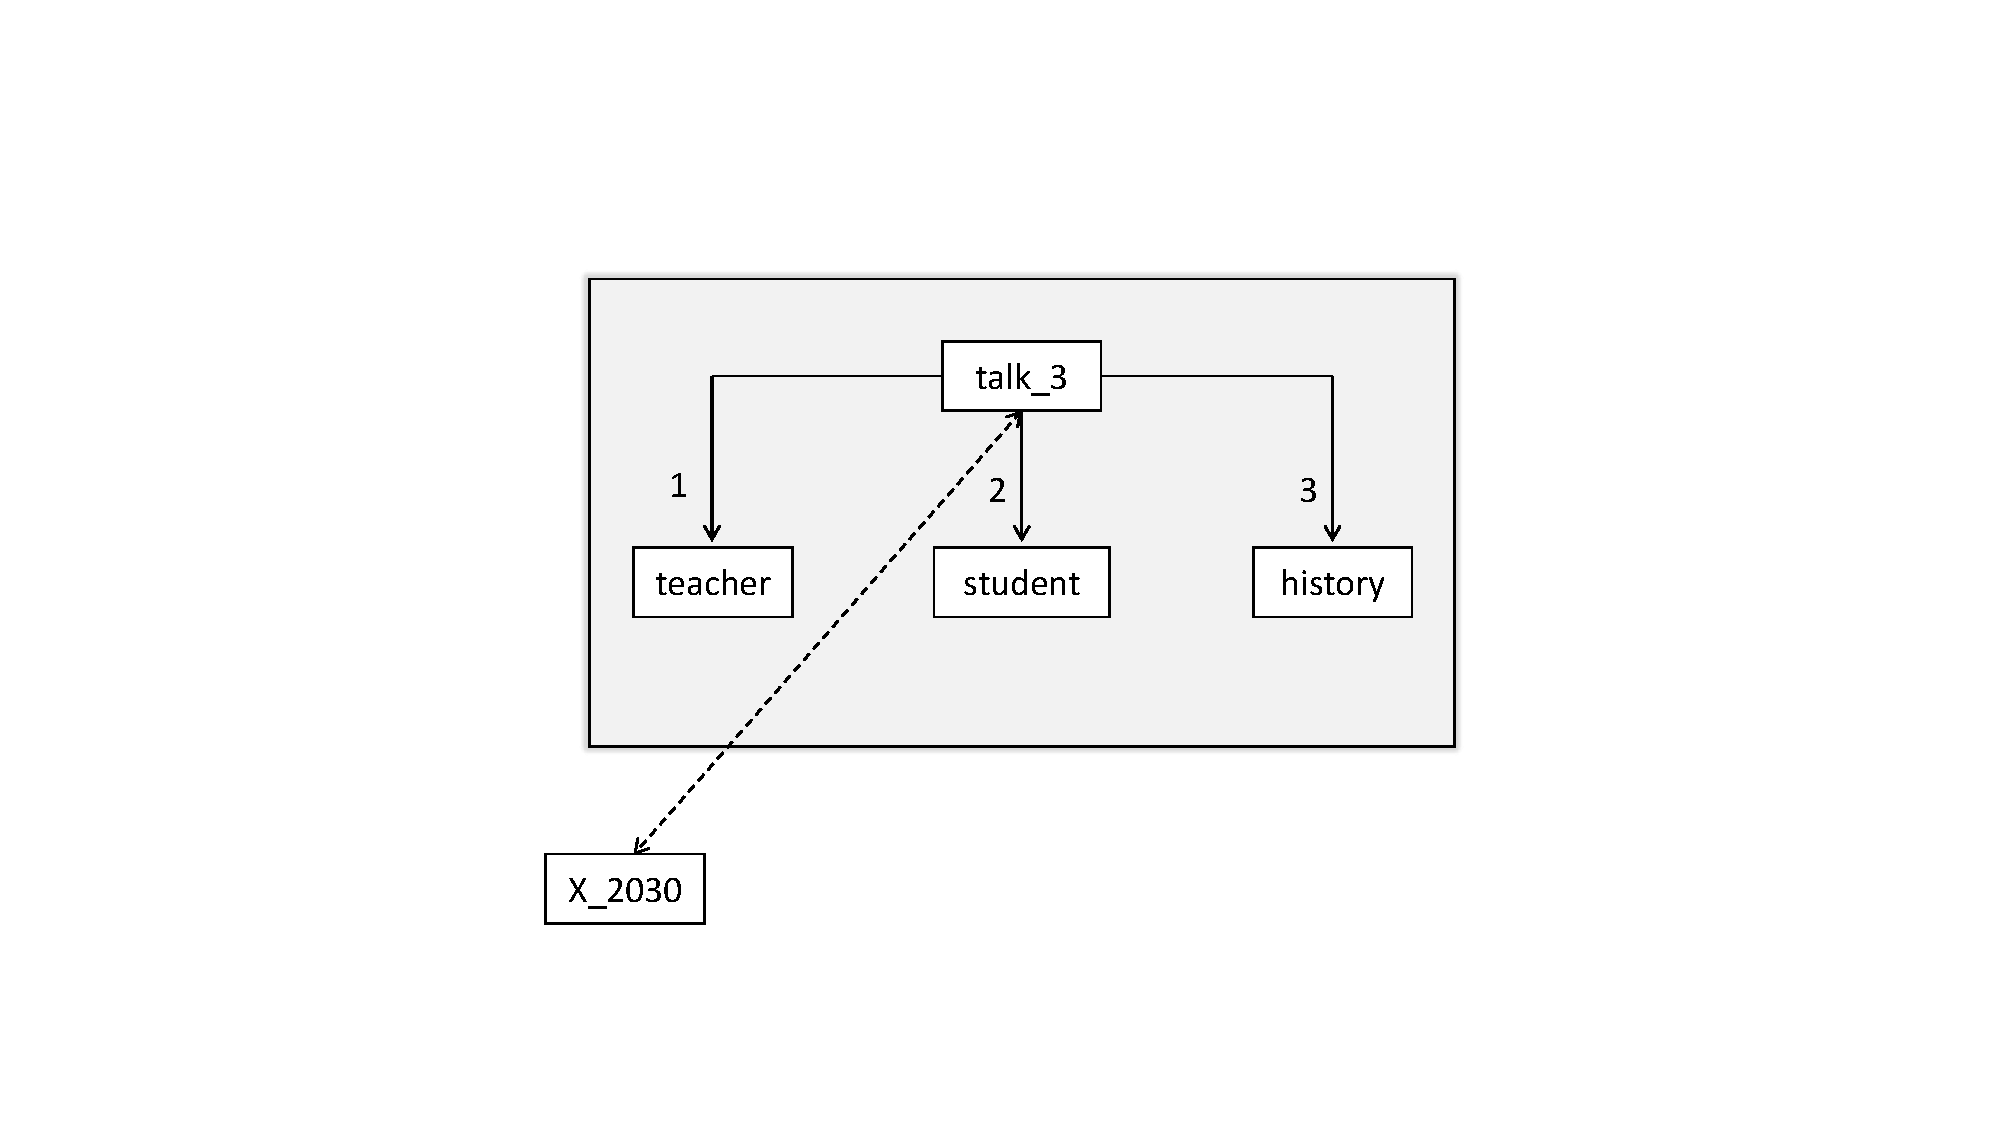
\includegraphics[width=1\textwidth, trim = {0cm 3.4cm 0cm 4.7cm},clip]{ch6/figs/root_implem.pdf}
	\caption{Création de la racine à partir du n\oe{}ud dominant}
	\label{deroulement0}
\end{figure}

\subsection{Sélection du patron de régime dans le lexicon}
Ensuite, la règle \emph{actant\_gp\_selection} (figure~\ref{deroulement1}) est déclenchée par l'apparition de \lex{talk\_3} pour satisfaire la racine. GenDR récupère les traits encodés pour chaque attribut \texttt{gp} de la classe verbale \texttt{talk-37.5}. Parmi ces \texttt{gp}, GenDR récupère ensuite le trait \texttt{id} dont la valeur est \texttt{NP\_V\_PP\_about\_topic\_PP\_to\_co\_agent} et le trait \texttt{dia} dont la valeur est \texttt{132}. Puis, il appose ces traits sur la racine.

\begin{figure}[htb]
	\centering
	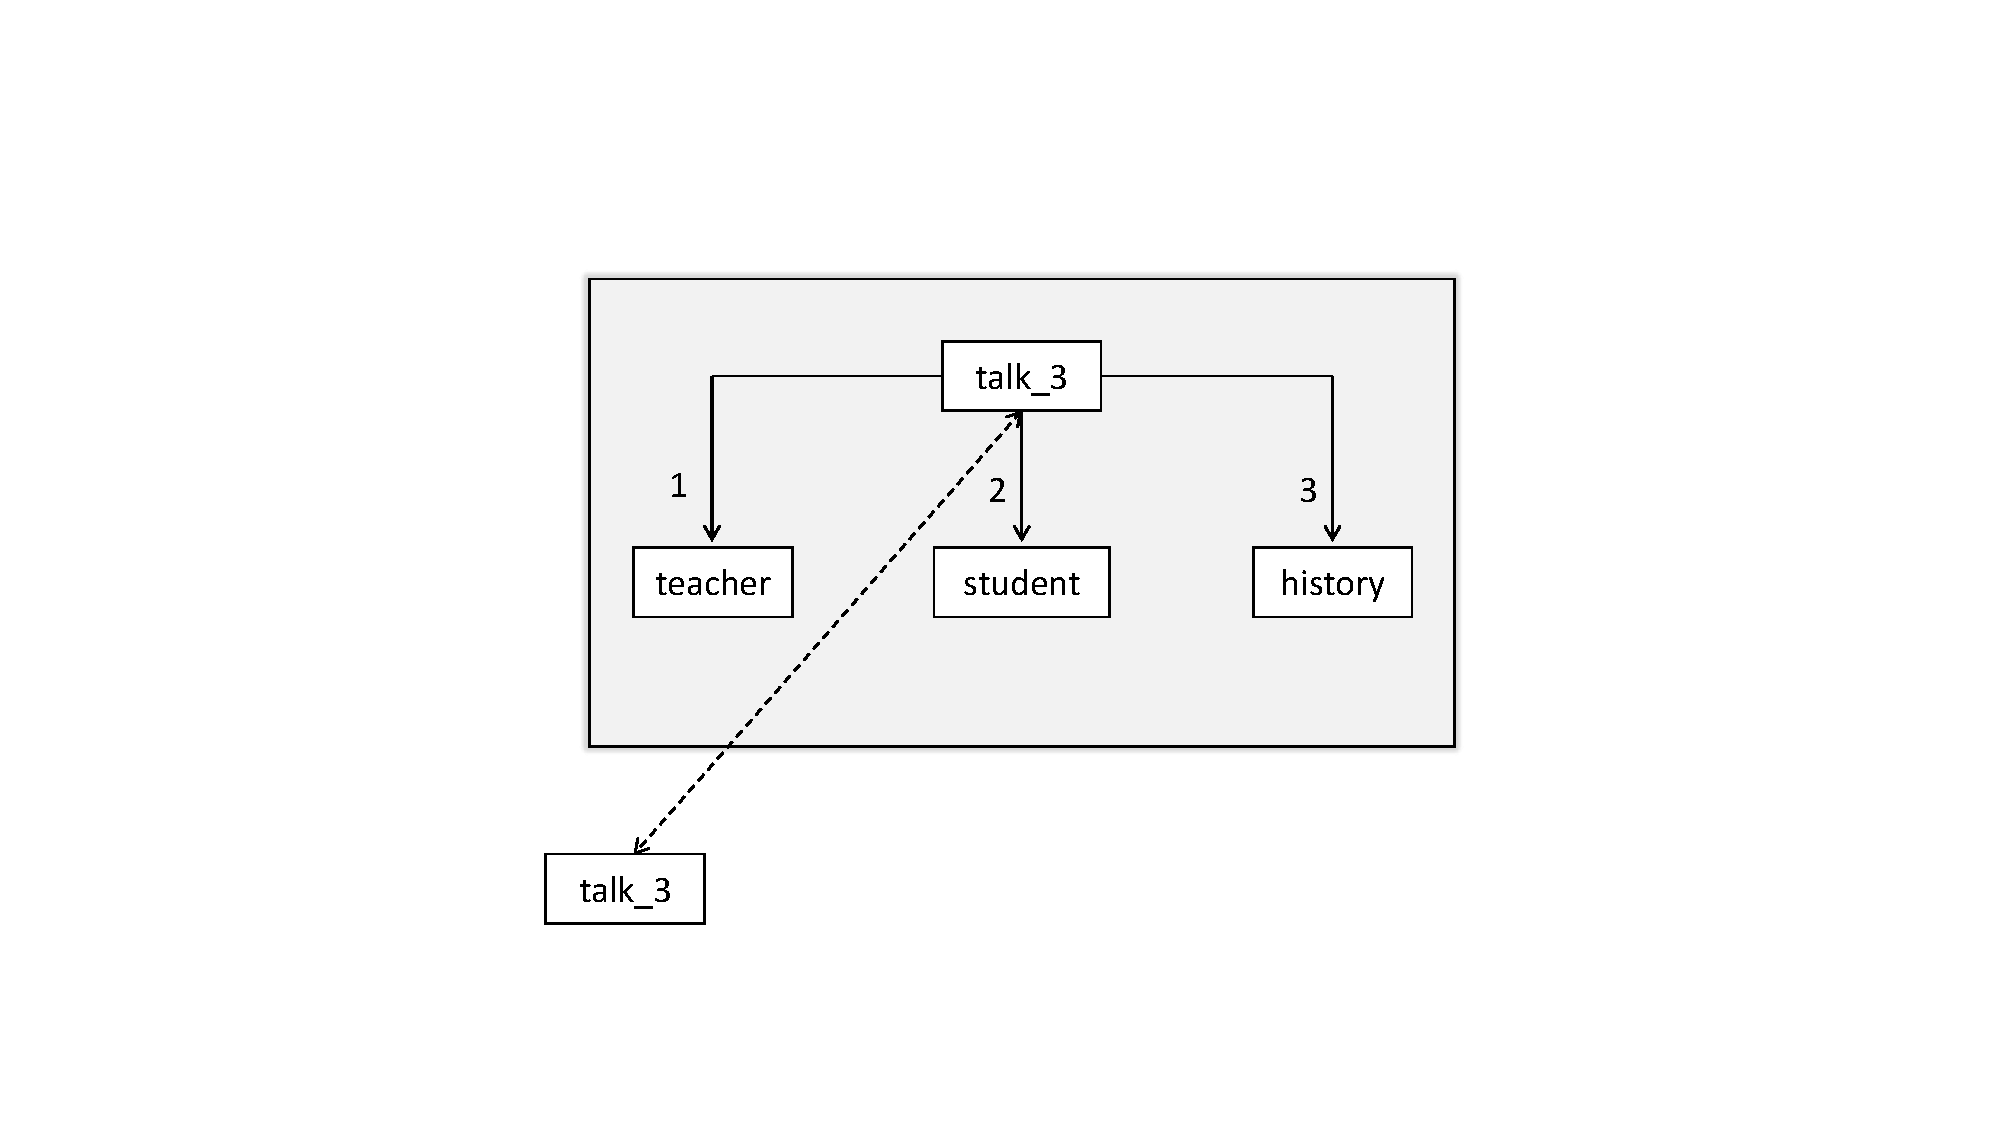
\includegraphics[width=1\textwidth, trim = {0cm 3.4cm 0cm 4.5cm},clip]{ch6/figs/lexical_root_implem.pdf}
	\caption{Sélection du patron de régime: \emph{actant\_gp\_selection}}
	\label{deroulement1}
\end{figure}

\subsection{Application de la règle actancielle: \emph{actant\_gp\_ijk}}
La règle \emph{actant\_gp\_ijk} est sélectionnée puisque le trait de diathèse apposé sur le n\oe{}ud précise qu'il y a trois actants sémantiques (figure~\ref{deroulement2}). À ce stade-ci, pour que l'arborisation se fasse correctement, il faut que les actants sémantiques imposés par la diathèse correspondent à ceux donnés par la structure sémantique. Comme notre exemple d'input en contient trois, alors la règle s'applique correctement et trois arcs en partance de la racine sont créés.

\begin{figure}[htb]
	\centering
	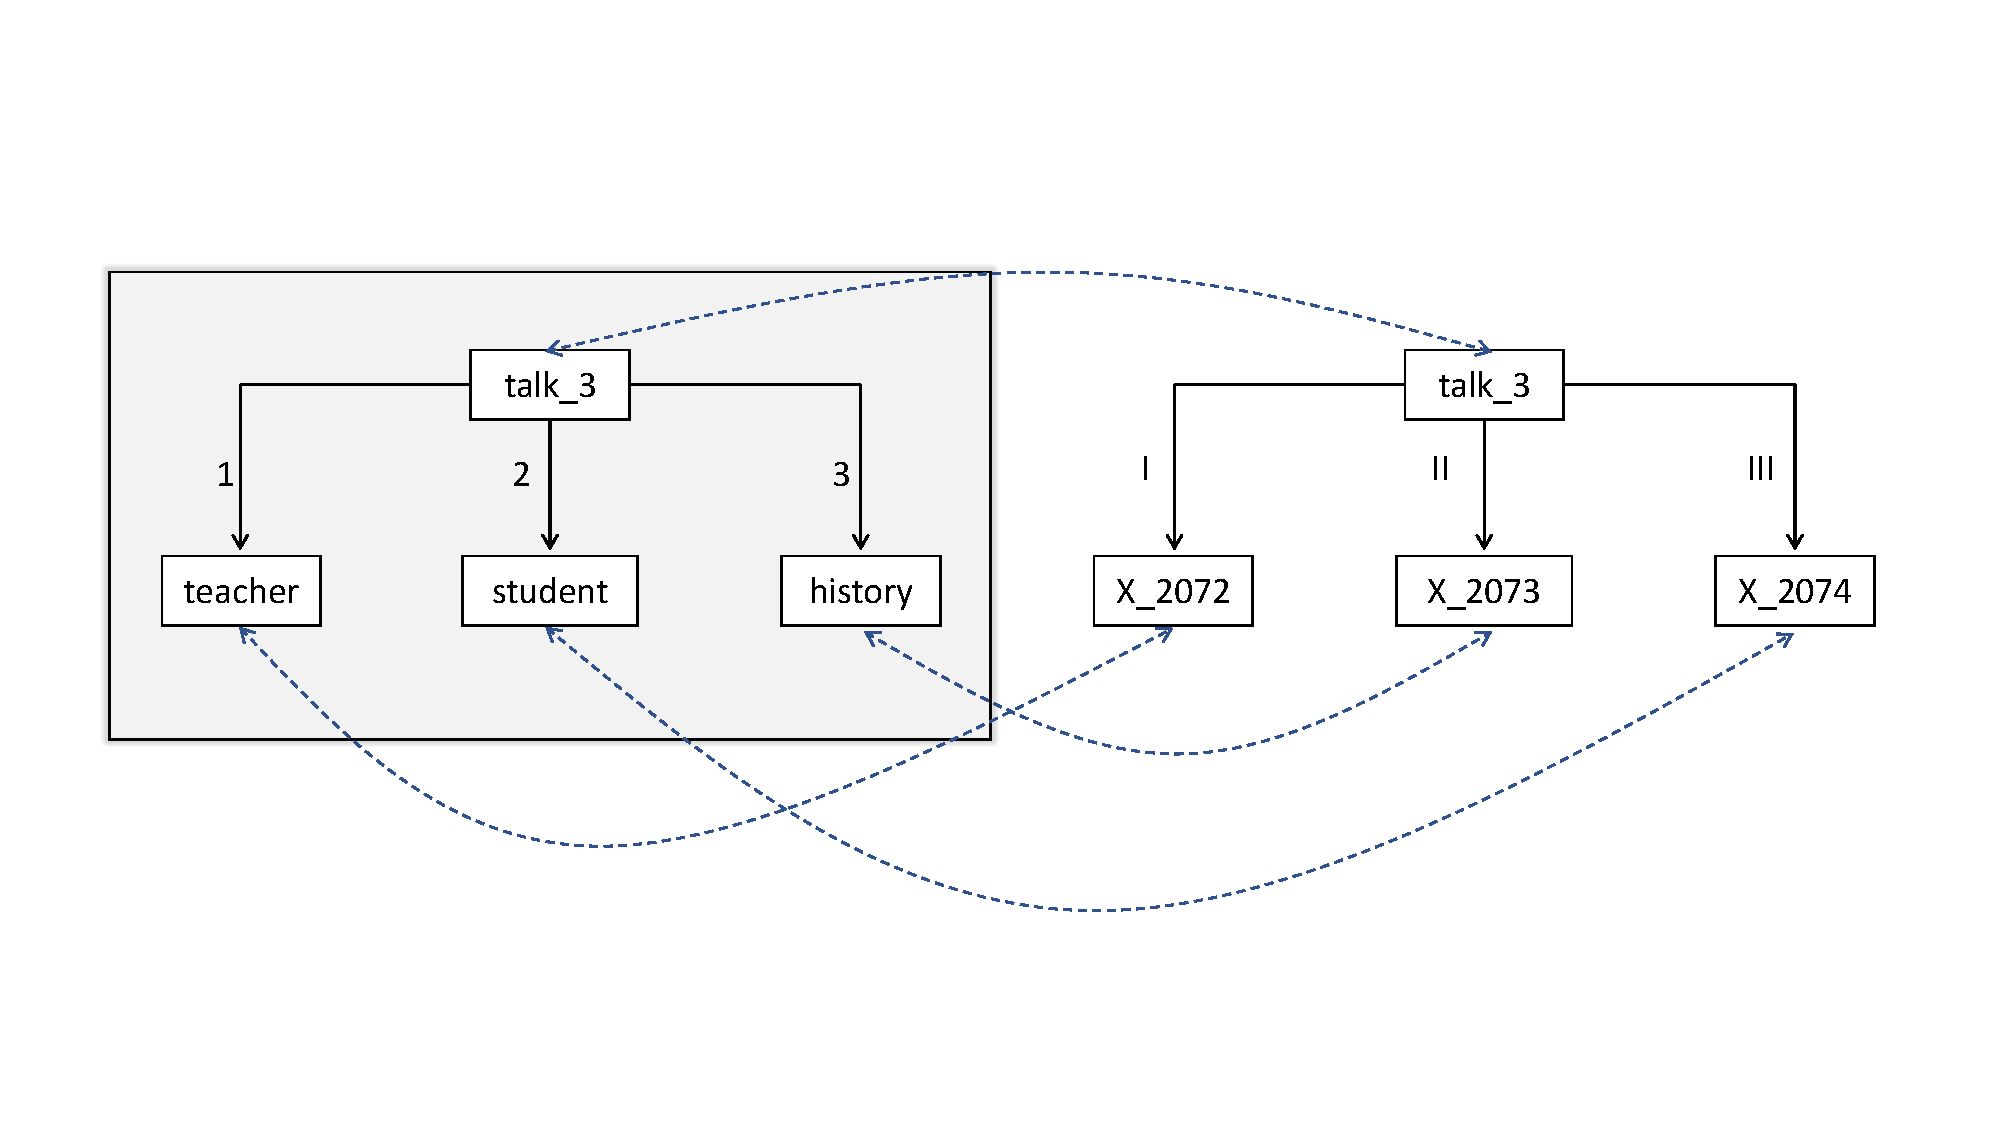
\includegraphics[width=1\textwidth, trim = {0cm 3.6cm 0cm 4.5cm},clip]{ch6/figs/actant_gp_ijk.pdf}
	\caption{Application d'une règle actancielle: \emph{actant\_gp\_ijk}}
	\label{deroulement2}
\end{figure}

\subsection{Application des contraintes sur les n\oe{}uds}
La règle de contrainte récupère les restrictions sur les actants syntaxiques que sélectionne \texttt{talk-3-1.5} grâce au \texttt{id} d'un de ses \texttt{gp} qui renvoient aux propriétés du patron de régime dans le \emph{gpcon}: \lstinline|NP_V_PP_about_topic_PP_to_co_agent { I={rel=subjective dpos=N}, II=...| (voir figure \ref{gpexemple}). Dans ce cas, la règle d'application de contraintes s'applique trois fois puisqu'il y a trois n\oe{}uds vides.

\subsection{Lexicalisation des n\oe{}uds contraints}
On lexicalise tous les n\oe{}uds puisqu'ils en respectent les contraintes. Le système utilisera une règle de lexicalisation simple dans ce cas parce que chacun de ces sémantèmes existe dans le \emph{semanticon} (voir la figure~\ref{deroulement3}).

\begin{figure}[htb]
	\centering
	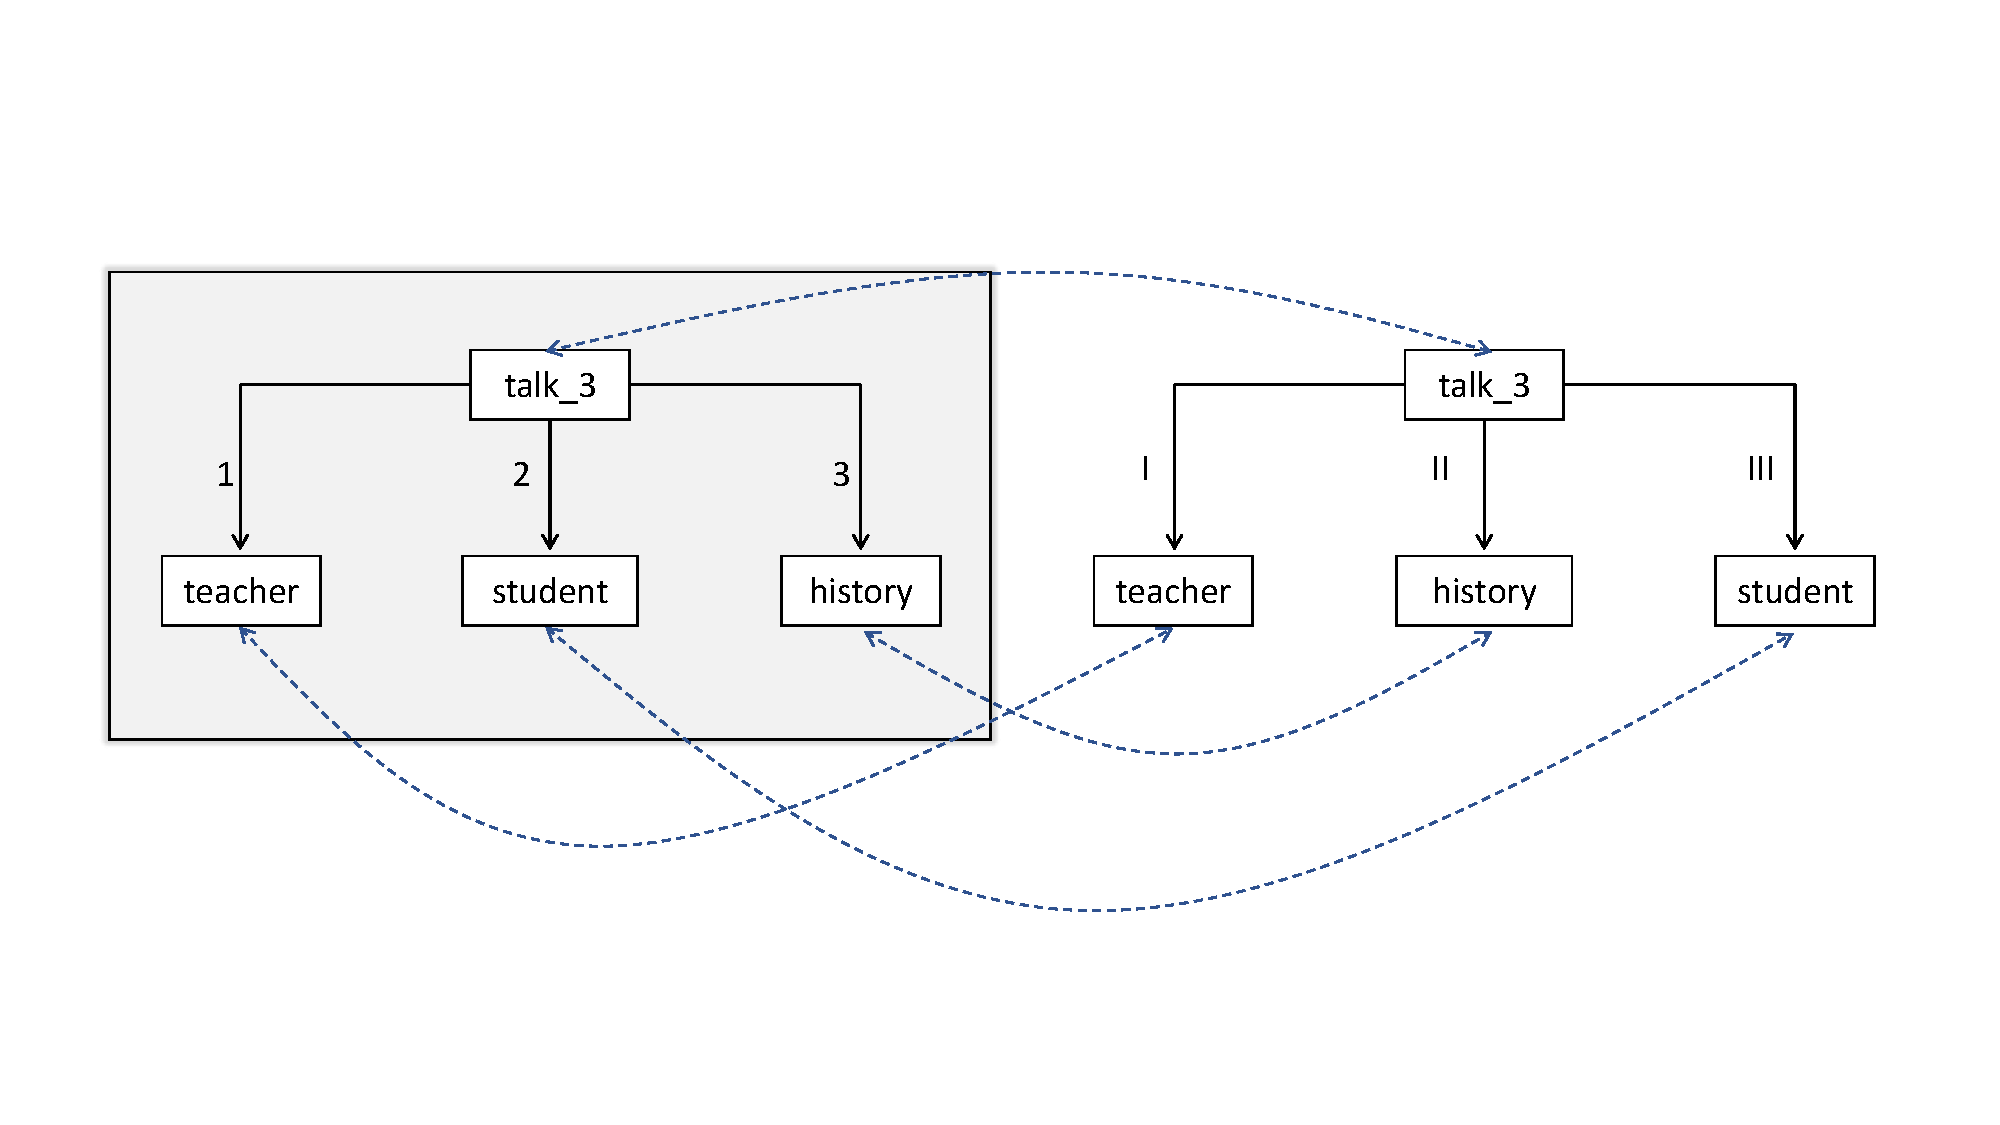
\includegraphics[width=1\textwidth, trim = {0cm 3.6cm 0cm 4.6cm},clip]{ch6/figs/actant_gp_lexical.pdf}
	\caption{Lexicalisation des n\oe{}uds contraints: \emph{lex\_standard}}
	\label{deroulement3}
\end{figure}

\subsection{Application de la règle \emph{actant\_gp\_selection}}
Finalement, la règle \emph{actant\_gp\_selection} est sollicitée pour les trois n\oe{}uds nouvellement lexicalisés \lex{teacher}, \lex{student} et \lex{history} (bien que l'arbre profond semble complet à cette étape). Comme toutes les catégories syntaxiques du lexique ont des patrons de régime, le système récupère systématiquement les traits \texttt{id} et \texttt{dia} de chaque lexème dans l'arbre au cas où ceux-ci sélectionneraient des actants à leur tour. Ce qui n'est pas le cas dans cet exemple (voir la figure~\ref{deroulement4}).

En ce qui concerne \textbf{l'arborisation de surface}, nous n'élaborerons pas sur cette partie puisqu'elle est quasi-identique à celle que nous avons vue dans la section \ref{sec:exemple} de GenDR. Les lexicalisations de surface sont effectuées par la même règle que nous avons expliquée, de même que la règle qui introduit les déterminants. Seules les règles actancielles de surface ont quelque peu changé, car elles puisent dorénavant l'information sur la correspondance entre les actants syntaxiques et les relations de surface qu'elles imposent (et le choix des prépositions) dans le \emph{gpcon}, alors que dans la version originale, le tout était encodé à même le \emph{lexicon}.

\begin{figure}[htb]
	\centering
	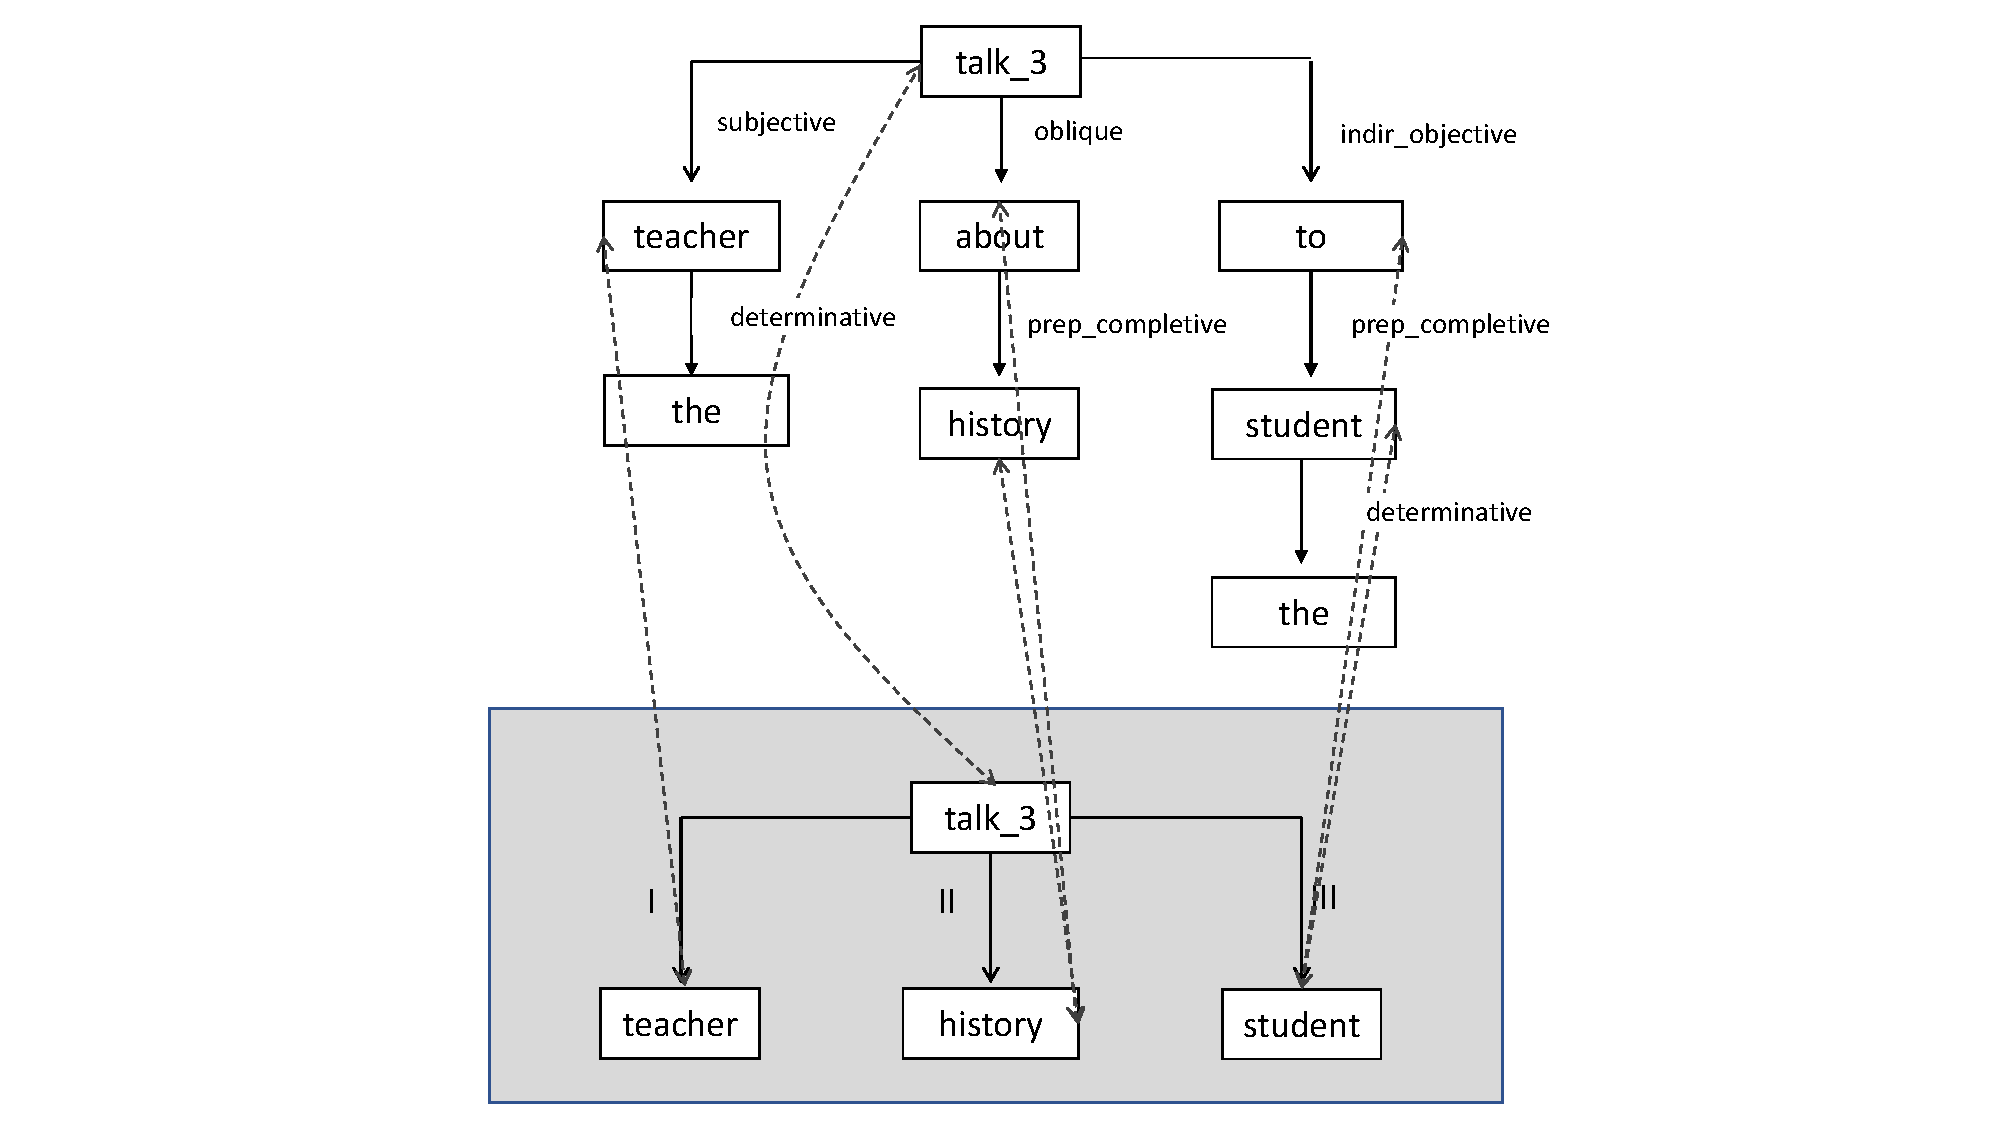
\includegraphics[width=1\textwidth, trim = {0cm 0.4cm 0cm 0.4cm},clip]{ch6/figs/final_implem.pdf}
	\caption{Applications des règles actancielles et réalisation des lexies fonctionnelles}
	\label{deroulement4}
\end{figure}

Cela met fin à notre chapitre sur l'adaptation de GenDR. Nous passerons maintenant à la phase d'évaluation.
%!TEX root = ../memoire.tex

\chapter{Évaluation}\label{ch:eval}

\cite{ReiterInvestigationValidityMetrics2009} expliquent qu'il existe trois types classiques d'évaluation en \ac{GAT}: l'évaluation basée sur l'exécution d'une tâche, l'évaluation automatique, puis l'évaluation humaine. Nous ferons un bref survol de ces trois types pour justifier quelle méthode nous avons choisi.

La méthode d'évaluation basée sur l'exécution de tâches consiste à trouver des évaluateurs qui exécuterons une tâche quelconque en se basant sur des rapports rédigés automatiquement. Dans ce contexte, on évalue directement l'impact des textes.  Les textes générés sont ainsi évalués en fonction de  Ainsi, il faut trouver des participants qui seront prêts à donner de leurs temps pour exécuter la tâche donnée. \cite{ReiterInvestigationValidityMetrics2009} estiment que c'est celle qui évalue le mieux le contenu des réalisations d'un système de \ac{GAT} puisqu'on peut mesurer concrètement si le texte généré est de bonne qualité. Par exemple, un texte bien composé permettra aux participants de réussir la tâche rapidement, tandis qu'un texte ilisible ou très mal écrit nuira grandement à la rapidité d'exécution de la tâche. Toutefois, c'est aussi la méthode la plus coûteuse en termes de temps et de ressources puisqu'il faut trouver des participants prêts à faire cette évaluation. Coûtent cher et sont généralement longs à entreprendre. Par exemple, quand c'est une tâche, l'évaluation est faite sur le nombre d'erreur. Ainsi, un bon texte génèrera moins d'erreurs, et un mauais texte plus.

Parmi les méthodes automatiques, la méthode BLEU, qui a été conçu à la base pour les systèmes de traductions automatique, semble très populaire en \ac{GAT}. Traditionnellement, dans un cadre de traduction automatique, il s'agissait de prendre une phrase tirée d'un corpus, en faire la traduction automatique et comparer le résultat avec la traduction de la même phrase, mais faite par un humain. En \ac{GAT}, le concept est similaire, il s'agit de parser \draft{la traduction qu'on me donne est 'analyser', est-ce que c'est bon ?} un texte d'un corpus, puis de fournir ce qui a été extrait à un système de \ac{GAT} puis de généré le texte, et finalement comparer le output automatique avec le texte original. \cite{Langkilde-gearyForestbasedstatisticalsentence2000} et \cite{Habash2003MatadorAL} ont utilisé cette méthode pour évaluer leurs systèmes. Toutefois, cette méthode d'évaluation est parfois critiquée, par exemple \cite{DBLP:conf/semeval/MilleCBW17} soulignent que BLEU évalue bien la couverture, mais ils critiquent leur évaluation de la qualité des outputs. Dans cet article, ils argumentent que leur réalisateur, FORGe, obtient un score au-dessus de la moyenne pour l'évaluation humaine, mais un score plus faible avec BLEU, et expliquent ce décalage par le fait que leur réalisateur favorise la précision par rapport au rappel.

L'évaluation humaine consiste à coter les outputs en fonction de leur performance à produire des phrases syntaxiquement et sémantiquement correctes selon les jugements des évaluateurs. \cite{BelzFirstSurfaceRealisation2011} ont proposent trois critères pour juger du texte généré automatiquement: la clareté, qu'on juge en fonction de la facilité à lire le texte, la lisibilité, qu'on juge par la fluidité du texte (construction syntaxique étranges, erreurs grammaticales,etc.) et la similarité de sens qui teste le paraphrasage. Cette méthode d'évaluation est plus simple à mettre en place que la méthode à base de tâche, mais elle demande plus temps à exécuter que la méthode automatique.
 
Considérant notre projet de recherche, les évaluations basées sur l'exécution de tâches ou sur les méthodes automatiques ne peuvent s'appliquer. D'abord, parce que notre système ne réalise pas du texte dans un but précis, donc nous n'avons pas de tâches à effectuer pour tester la validité des réalisations. De plus, nous ne génèrons pas du texte linéarisé, donc il faudrait trouver des participants capables de lire des arbres de dépendances. Pour cette même raison, nous ne pouvons pas utiliser la méthode automatique puisqu'on ne peut pas comparer automatiquement nos arbres de dépendances de surface avec des textes linéarisés écrits par des humains. Bref, la seule méthode d'évaluation qui s'offre à nous est l'évaluation humaine et c'est elle que nous avons employé.

\section{Méthodologie d'évaluation}

Pour procéder à l'évaluation de notre système, nous avons construit 978 graphes sémantiques représentant les phrases exemples extraites de VerbNet (voir section \ref{sec:pythonstruc}) et nous en avons passé un échantillon à GenDR. Le but était de tester la qualité et la couverture de GenDR sur la base de deux critères: le rappel et la précision.

Pour mener à bien notre évaluation, nous avons pris un échantillon des 978 structures car nous étions limité par le temps. Ainsi, 75 structures furent choisies aléatoirement dont 25 ont servi pour une phase de \emph{développement} précédant la phase d'évaluation, pour vérifier quels étaient les problèmes immédiats et les corriger avant d'entamer la partie \emph{évaluation}. La phase de développement nous a permi de constater que de nombreux inputs comportaient des erreurs d'encodage, ce qui nous a forcé à vérifier que chacun des inputs de la partie \emph{évaluation} soit impeccable. De plus, la partie \emph{développement} nous a aussi permi de constater que certains lexèmes, appartenant à des parties du discours différentes, apparaissaient en double dans notre dictionnaire. Nous avons conséquemment procédé à un filtrage pour les retrouver et nous avons remédier à la situation. Par exemple, le verbe \lex{work} et le nom \lex{work} ont le même signifiant, donc le système ne sait pas comment les différencier. Nous avons ainsi désambiguïser chacun d'entre eux en les encodant comme deux lexèmes différents ayant le même signifié, généralement en encodant les noms comme \lex{work} de cette manière \lex{work\_n}. 

Ensuite, après la phase de développement terminée, il ne nous restait qu'à passer à la phase d'évaluation sur sur les 50 structures restantes.
                              
\section{Rappel}
\draft{centrer les tableaux}
Nous avons mesuré le rappel en considérant le nombre de structures attendues que GenDR a généré par rapport au nombre de structures attendues. Dans ce contexte, une \scare{structure attendue} est une structure qui devrait normalement être générée par notre système lorsqu'un \ac{GP} permet sa réalisation. Ainsi, chaque structure manquante à l'appel est considérée comme une erreur.
\[\text{Rappel} = \frac{\text{nombre de structures attendues générées}}{\text{nombre de structures attendues}}\]

\begin{table}
\caption{Données du rappel}
\begin{tabular}{ |p{6cm}||c|c|  }
 \hline
 \multicolumn{3}{|c|}{Rappel} \\
 \hline
  & RSyntP & RSyntS\\
 \hline
 Nombre de structures attendues   & 120  &127  \\
 Nombre de structures générées &  118  & 120   \\
 Erreurs de GenDR & 0 & 0\\
 Erreurs de VerbNet    & 0 & 5\\
 Incompatibilité TST/VerbNet & 2 & 2\\
 Pourcentage global & 98\%  & 94\% \\
 Pourcentage GenDR & 100\%  & 100\% \\
 \hline
\end{tabular}
\end{table}

Nous avons fait des tests à la fois pour la RSyntP et la RSyntS, puisque GenDR réalise des arbres pour chacune de ces représentations. Comme les résultats changeaient quelque peu en fonction de la représentation, nous avons jugé pertinent de le démontrer. Certaines erreurs ne sont pas visibles en syntaxe profonde, notamment lorsqu'il s'agit de prépositions. 

D'abord, à la lecture du tableau, on remarque que GenDR a un bon rappel. En effet, les scores sont excellents et cela est dû à notre système qui fonctionne à base de règles. \draft{élaborer un ti peu plusse}

Ensuite en ce qui concerne les erreurs de VerbNet en syntaxe profonde, il n'en y en a pas, mais 5 structures attendues n'ont pas été générées en surface. Ces erreurs de surface sont dues au fait que quelques verbes utilisés dans les phrases d'exemples de VerbNet ne figurent pas dans la base de données. Par le fait même, les \acp{GP} associés à ces verbes ne sont pas connus de GenDR, ce qui mène à l'impossibilité de générer l'arbre attendu. C'était le cas par exemple de la structure 077-\form{He begged her to do it}, où le verbe \lex{do} n'a pas d'entrée dans VerbNet. Les autres erreurs de VerbNet sont similaires, mais au lieu que ce soit une entrée verbale qui manque, c'est un \ac{GP} qui est absent. Cela fait en sorte que la structure à laquelle on s'attendrait ne sera pas générée puisque GenDR appliquera un \ac{GP} par défaut, mais les chances sont que ce ne soit pas le bon. Par exemple, nous avions la phrase 974-\form{He backed out of going on the trip}, mais aucune des acceptions de \lex{go} ne contenait le régime nécessaire pour réaliser cette phrase.

Finalement, les autres erreurs proviennent d'incompatibilités théoriques entre VerbNet et la \ac{TST}. En effet, nous avons représenté chaque phrase exemple en graphe sémantique à la \cite{mel2012semantics}. Comme les patrons de régime font le pont entre la sémantique et la syntaxe, s'il y a une incompatibilité entre la sémantique de l'énoncé et sa représentation syntaxique selon VerbNet, ça mènera à un échec. Par exemple, la phrase \form{The plays and ballets alternate} se traduit par la combinaison du verb \lex{alternate} un seul actant syntaxique (le NP \emph{plays and ballets}) selon VerbNet. Comme l'input sémantique que nous avons fourni au système contenait deux actants sémantiques, le \ac{GP} qui régit la construction (\texttt{NP\_V}) ne peut pas faire le pont entre notre interprétation sémantique et les constructions fournies par VerbNet. Toutefois, en \ac{TST}, nous considérons qu'il y a deux actants sémantiques, donc deux actants syntaxiques puisqu'ils sont réalisés en surface. Malgré tout, notre système est capable de générer 036-\form{Plays alternate with ballets}, ce qui démontre la flexibilité du système.

\section{Précision}
\draft{centrer les tableaux}
Pour mesurer la précision, nous avons considéré le nombre de structures correctes générées (correctes signifiant grammaticales), par rapport au nombre de structures générées (peu importe leur grammaticalité). Autrement dit, chaque structure agrammaticale générée correspond à une erreur.
\[\text{Précision} = \frac{\text{nombre de structures grammaticales}}{\text{nombre de structures générées}}\]

\begin{table}
\caption{Données de la précision}
\begin{tabular}{ |p{6cm}||c|c|  }
 \hline
 \multicolumn{3}{|c|}{Précision} \\
 \hline
  & DSynt & SSynt\\
 \hline
 Nombre de structures générées   & 120  &127  \\
 Nombre de structures correctes &  101  & 100   \\
 Erreurs de GenDR & 0 & 3\\
 Erreurs de VerbNet    & 18 & 23\\
 Incompatibilité TST/VerbNet & 1 & 1\\
 Pourcentage global & 83\%  & 77\% \\
 Pourcentage GenDR & 100\%  & 97\% \\
 \hline
\end{tabular}
\end{table}

Les trois erreurs de GenDR en surface proviennent du fait que certaines structures à deux verbes nécessitent la présence d'un PRO qui agit comme le premier actant du second verbe, puisque nous ne pouvons pas faire de construction triangulaire dans GenDR pour l'instant \draft{faire un exemple dans PowerPoint}. Le problème est qu'en surface, le PRO disp Incapable de faire disparaître le PRO en surface, il manque une règle pour faire ça.

Parmi les informations lexicales extraites de VerbNet, certaines nous ont aussi fait réaliser des phrases quasi-correctes mais bizarres. Cela est une conséquence des \acp{GP} qui permettent de deux à quatre prépositions différentes pour la réalisation d'un même actant. Le système va donc générer plusieurs arbres différents en fonction des prépositions possibles, mais généralement seule l'une d'entre elles donne une phrase grammaticale. Ainsi, en appliquant les\acp{GP} de VerbNet, GenDR génère les phrases \form{The doctor cured pat of pneumonia} et \ungr\form{The doctor cured pat out of pneumonia} str 177 .

problèmes: VerbNet a pas le bon gp, donc les phrases qui sont réalisées sont agrammaticales : "he backed out of going" str 974, 
utilisation d'un gp qui rend la phrase agramamticale. VerbNet a plusierus gp dans une classe verbale qui devraient tous bin fonctionnés, mais pas tjs "`barry cryer erased at the writing"' str 968 I ended, I ended with a speech str 843

DO n'Est pas encodé dans verbnet, donc GenDR tente des trucs, dont le considéré comme un N, et ça donne "I begged her for the DO"'

Problème de GenDR: on ne peut pas traiter les constructions triangulaires, donc on fait appel à un Pro lorsqu'il y a deux verbes. Et il nous faut un mécanisme pour supprimer le PRO en SSynt. L'arbre en soi était bon, mais il y avait un PRO qui flottait tout seul dans la réalisation finale. 

\draft{mécanisme d'héritage (le documenter) (l'écrire au chap 4) et le rectifier au chap 5.

se baser sur le manuel pour parler du core, plus la présentation, présenter chaque règle et son fonctionnement de façon abstraite. Présenter les règles, pas l'exemple, il sert à appuyer la description.

relire les marqueurs comme d'ailleurs, effectivement, brièvement,etc. (reformuler plus clairement), zapper les mots vides}

% !TEX root = ../memoire.tex

\chapter*{Conclusion}
L'un des enjeux fondamentaux en \ac{GAT} est de générer du texte qui paraisse aussi naturel que possible. Généralement, il faut pour cela que le système ait accès à des connaissances linguistiques fines. Par exemple, les réalisateurs à base de règles nécessiteront une grammaire qui modélise des phénomènes complexes et des dictionnaires riches encodant les propriétés de combinatoires des lexies. Si on veut couvrir le plus de constructions permises par une langue, il nous faut avoir accès aux différents comportements des lexèmes de cette langue. Certaines parties du discours présentent des comportements plus prévisibles, mais les comportements syntaxiques des verbes sont extrêmement variés et très imprévisibles. Il faut donc stocker ces données dans un dictionnaire pour pouvoir produire du texte représentant toute la richesse des langues naturelles.

C'est pour cette raison que plusieurs chercheurs ont cherché à créer des ressources lexicales décrivant les comportements syntaxiques des unités lexicales de l'anglais. Ces ressources ont pour but de servir toutes les branches du \ac{TAL}, dont la \ac{GAT}. L'objet de ce mémoire était de pourvoir GenDR d'une couverture linguistique beaucoup plus grande que celle qu'il a présentement en y intégrant VerbNet, qui est une base de données lexicales décrivant les comportements syntaxiques de 6\,393 verbes. Ainsi, ce mémoire répond à ces deux questions:

\begin{enumerate}
  \item \form{Comment implémenter une telle ressource dans un réalisateur profond à base de règles ?}
  \item \form{Est-ce que cette implémentation donne de bons résultats ?}
\end{enumerate}

Dans le premier chapitre, nous introduisons la \ac{GAT} et le pipeline classique qui la compose. Nous nous sommes arrêté sur la réalisation linguistique, qui est la dernière étape du pipeline. Ensuite nous avons souligné qu'il existait différents types d'approches pour effectuer la réalisation linguistique: à base de patrons, à base de règles et à base de modèles statistiques. Ensuite, nous avons exploré les différents réalisateurs de surface et profonds. Notamment, nous avons parlé de SimpleNLG \citep{GattSimpleNLGRealisationEngine2009}, JSrealB \citep{MolinsJSrealBBilingualText2015} et RealPro \citep{LavoieFastPortableRealizer1997} qui sont des réalisateurs de surface. Puis, nous avons décrit des réalisateurs profonds: KMPL \cite{BatemanEnablingTechnologyMultilingual1997}, SURGE \citep{Elhadad98surge:a}, MARQUIS \citep{WannerMARQUISGENERATIONUSERTAILORED2010}, FORGe\citep{MilledemoFORGePompeu2017}.

Dans le deuxième chapitre, nous avons décrit en détail le réalisateur profond GenDR \citep{lareau18}, un héritier de MARQUIS. Nous avons dépeint l'environnement dans lequel GenDR s'insère: le logiciel MATE (conçu pour la TST), qui offre un éditeur de graphes, de dictionnaire et de règles pour développer et tester une grammaire computationnelle. Ensuite nous avons expliqué quelques notions de base de la \ac{TST} dont l'interface sémantique-syntaxe. Puisque GenDR opère au niveau de cette interface en modélisant l'arborisation et la lexicalisation. Finalement, nous avons démontré le fonctionnement du réalisateur GenDR à l'aide d'un exemple décrivant l'interaction des règles et dictionnaires pour générer des arbres syntaxiques de surface à partir d'un input sémantique.

Dans le troisième chapitre, nous avons fait un survol des ressources lexicales potentielles que nous envisagions pour augmenter la couverture de GenDR et sa capacité à traiter le plus grand nombre de constructions possibles. Nous avons exploré notamment WordNet, FrameNet, XTAG, LCS, Comlex, Valex,et le VDE et finalement VerbNet, le grand gagnant, qui est basé sur les travaux de \cite{verb-classes.levin.1993}. Ce qui nous a plu dans cette ressource est l'organisation des classes verbales ainsi que sa large couverture (plus de 6\,000 verbes désambiguïsés).

Dans le quatrième chapitre, nous avons procédé à l'extraction des données lexicales de VerbNet. Nous avons d'abord extrait les informations syntaxiques des classes verbales en conservant la hiérarchie pensée pour VerbNet. Puis nous avons extrait les verbes associés à chaque classe verbale et nous les avons désambiguïsés avant de les ajouter à notre dictionnaire. Ensuite, nous avons procédé à la création du dictionnaire de patrons de régime à partir des données extraites. Le tout a été fait par l'entremise de Python, qui nous a permis de manipuler les fichiers de VerbNet encodés en \emph{XML}.

Dans le cinquième chapitre, nous avons démontré comment nous avons adapté GenDR à l'utilisation d'un dictionnaire de patrons de régime. Le nombre de verbes décrit par le réalisateur est ainsi passé de 500 à 6\,393. Puis, nous avons complètement changé l'utilisation des patrons de régime avec la venue du dictionnaire de \acp{GP}. Cela a permi à GenDR d'avoir une couverture beaucoup plus large en termes de lexèmes verbaux et de couvrir un grand nombre de constructions syntaxiques possibles en anglais. Par le fait même, on règle le problème des \acp{GP} multiples.
	
Dans le sixième chapitre, nous avons montré comment nous avons créé les scripts permettant de générer les structures de base pour évaluer GenDR. Nous avons sélectionné 50 structures sémantiques aléatoirement parmi les 978 encodées pour faire l'évaluation. Nous avons d'abord testé notre système en calculant le rappel et la précision. D'abord, le rappel a été calculé en vérifiant qu'on arrivait à générer les structures syntaxiques des 50 phrases attendues. Ensuite, la précision a été calculée en vérifiant combien des structures générées étaient grammaticales. Les résulats nous montrent que les règles de GenDR fonctionnent généralement bien et que la plupart des erreurs viennent de VerbNet, notamment les erreurs affectant la précision.

Le travail que nous avons fait apporte plusieurs contributions importantes au développement de GenDR. Nous avons démontré comment s'implémente une ressource lexicale comme VerbNet dans un réalisateur profond à base de règles, de façon surtout automatique. Nous avons montré qu'il est possible de prendre une ressource relativement neutre d'un point de vue théorique et d'adapter les données pour une utilisation dans un autre cadre théorique sans que ce ne soit trop encombrant. C'est ainsi que nous avons créé un dictionnaire de patrons de régime selon le formalisme de la \ac{TST}. Cela pourrait être utile à d'autres réalisateurs qui voudraient s'inspirer de cette théorie. De plus, nous avons montré que l'implémentation de VerbNet sans trop de retouches donnait un score naturel de 80\% de précision, ce qui veut dire que l'intégration de cette ressource dans le cadre de la \ac{GAT} nécessite quelques modifications pour éviter des phrases agrammaticales. Il reste que la couverture de GenDR s'est vue grandir d'un coup grâce à l'implémentation massive de VerbNet, ainsi il est possible de rapidement augmenter la couverture d'un réalisateur, sans trop modifier la source. 

Cette recherche contribue également à évaluer la pertinence de VerbNet comme dictionnaire verbal pour un réalisateur profond en \ac{GAT}. Nous en concluons que c'est une ressource que se prête très bien à cette branche du \ac{TAL}, mais qu'il faudrait faire quelques modifications à la ressource post-intégration pour tenir compte des erreurs que nous avons soulignées.

De plus, ce projet de recherche démontre que GenDR pourrait aussi bénéficier d'autres ressources lexicales pour complémenter sa couverture. Notamment, nous pourrions implémenter les régimes des noms, grâce aux autres ressources (comme FrameNet \cite{FillmoreBackgroundFramenet2003a}). Nous pourrions aussi aller chercher les \acp{GP} manquants dans d'autres ressources que nous avons répertoriées. De plus, comme il existe des VerbNet dans d'autres langues (francais \citep{danlos:hal-01179175}, portugais \citep{ScartoncrosslinguisticVerbNetstylelexicon2012}, italien \citep{busso2016italian}, espagnol \citep{TauleAnCoraNetMappingSpanish2010}, tchèque \citep{pala2008can}, mandarin \citep{liu2008construction}), on aurait avantage à les acquérir. La tâche serait relativement rapide puisqu'on sait déjà comment implémenter les données de ce format. Comme GenDR est un réalisateur multilingue, son architecture interne est déjà établie pour accueillir d'autres langues. Finalement, une recherche récente \citep{Majewska2017} démontre que l'exportation des classes et des membres de VerbNet \citep{SchulerVerbnetBroadcoverageComprehensive2005} à d'autres langues est valide et donne généralement de bons résultats. Ils soulignent qu'il faudrait évidemment faire des ajustements spécifiques pour chaque langue, mais que l'architecture pensée pour l'anglais se traduit bien à d'autres langues. 

Finalement, pour que GenDR soit utilisé à pleine capacité, il faudrait lui intégrer le module de fonctions lexicales de sa version originale \citep{LambreyImplementationcollocationspour2017, lareau18}, ce qui enrichirait nettement sa nouvelle version grâce à la modélisation des règles permettant le traitement des collocations.


% Annexes
% Enlever le commentaire de \appendix pour faire vos annexes.
% Les annexes sont ensuites faites comme un chapitre normal : \chapter{nom_de_l'annexe}.
\appendix

%%%%%%%%%%%%%%%%%%%%%%%%%%%%%%%%%%%%%
%%   BIBLIOGRAPHIE                  %
%%%%%%%%%%%%%%%%%%%%%%%%%%%%%%%%%%%%%
  % Enlever les commentaires de la prochaine commande si vous préférez que le
  % chapitre s'appelle « Références » plutôt que « Bibliographie » (au choix selon le contexte).
%\let\bibname=\refname   

%% Lorsque vous serez prêt à faire afficher votre bibliographie
%% et vos références, enlevez les commandaires des commandes suivantes
%% et donnez le nom de votre fichier .bib à la commande \bibliography{..}
%% (consultez l'exemple au besoin).  Vous pouvez utiliser le style de votre
%% choix.  Le fichier francaissc.bst est inclus avec le gabarit.  Vous pouvez
%% utiliser ce style avec  \bibliographystyle{francaissc}
% 
\bibliographystyle{biblio/francaissc}		    % Le style de la bibliographie. Notons que les extensions ne sont pas données pour ces deux fichiers.
\bibliography{biblio/references}		    % La base de données contenant des entrées bibliographiques. Seules celles référencées dans le texte seront ajoutées \`a la bibliographie.

%!TEX root = ../memoire.tex

\chapter{Corpus d'évaluation}

Inputs et outputs de GenDR à partir des phrases tirées de VerbNet

\iffalse 
\begin{longtable}{@{}rp{10cm}@{}}
\caption{Phrases tirées de VerbNet pour l'évaluation}\\
\toprule
\textbf{Num} & \textbf{Phrase} \\
\midrule
\endfirsthead
\multicolumn{2}{c}%
{\tablename\ \thetable\ -- \textit{Suite}} \\
\toprule
\textbf{Num} & \textbf{Phrase} \\
\midrule
\endhead
\bottomrule \multicolumn{2}{r}{\textit{Suite à la page suivante}} \\
\endfoot
\bottomrule
\endlastfoot

17	&	I loved writing \\
27	&	They allow smoking \\
36	&	Plays and ballets alternate \\
77	&	I begged her to do it \\
111	&	The dragon breathed fire on Mary \\
142	&	Oils's price increased ten percent \\
177	&	The doctor cured Pat of pneumonia \\
198	&	She classified the works as `dangerous' \\
206	&	Cora coiled the rope around the post \\
213	&	The prime minister complained to the former president about U.S. interference in his country's affairs \\
222	&	The Milky Way comprises more than 100 billion planets \\
227	&	The children hid from Sally \\
244	&	They considered him professor \\
250	&	I spent the time on worries \\
264	&	Some of the members may donate privately \\
267	&	He converted to believing in Buddha \\
330	&	This flyer and that flyer differ \\
384	&	He entered the room \\
399	&	The bells traded places \\
426	&	We focused on it \\
428	&	We brooded about it \\
452	&	Carmen bought a dress for \$50 \\
476	&	The teacher gathered the kids \\
503	&	Smith was inscribing \\
540	&	We abandoned the area \\
554	&	Sasha dawdled in the museum \\
581	&	I anguished over Aslan's pain \\
583	&	Dina masqueraded as a lawyer \\
604	&	Herman added a computer to the network \\
618	&	I neglected to do the job \\
630	&	She laughed in embarrassment \\
667	&	Lydia pocketed the change in her left pocket \\
686	&	Donna grilled me steaks \\
688	&	The dealer valued the book \\
746	&	Tom jumped the horse over the fence \\
750	&	The horse jumped the stream \\
777	&	TransCanada is shifting its HQ to Calgary from Toronto \\
789	&	The crew spotted the island \\
836	&	The thief stole the paint for Mary \\
843	&	I ended the party with a speech \\
845	&	Winnie the Pooh subjugated the unfortunate Pixies \\
851	&	The streets gushed with water \\
862	&	The sailor drowned \\
868	&	Bees are swarming in the garden \\
873	&	Paula swatted the fly with a cloth \\
894	&	Ellen told Helen a story \\
900	&	Steve tossed the ball from the corner to the garden \\
955	&	Linda winked her eye \\
968	&	Barry Cryer erased the writing \\
974	&	He backed out of going on the trip \\

\end{longtable}
\fi

\begin{tabbing}
(17)\quad\= \emph{I loved writing.} \\
\> \begin{minipage}{16cm}
\raisebox{-0.5\height}{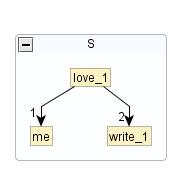
\includegraphics[scale=0.45]{{annexes/figs/test-eval-17.sem}.jpg}}
\raisebox{-0.5\height}{~$\Rightarrow$~}
\raisebox{-0.5\height}{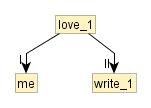
\includegraphics[scale=0.45]{{annexes/figs/test-eval-17.dsynt}.jpg}}
\raisebox{-0.5\height}{~$\Rightarrow$~}
\raisebox{-0.5\height}{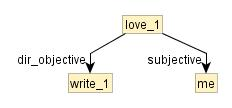
\includegraphics[scale=0.45]{{annexes/figs/test-eval-17.ssynt}.jpg}}
\end{minipage}
\end{tabbing}

\begin{tabbing}
(27)\quad\= \emph{They allow smoking.} \\
\> \begin{minipage}{16cm}
\raisebox{-0.5\height}{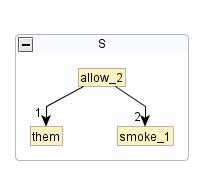
\includegraphics[scale=0.45]{{annexes/figs/test-eval-27.sem}.jpg}}
\raisebox{-0.5\height}{~$\Rightarrow$~}
\raisebox{-0.5\height}{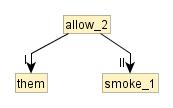
\includegraphics[scale=0.45]{{annexes/figs/test-eval-27.dsynt}.jpg}}
\raisebox{-0.5\height}{~$\Rightarrow$~}
\raisebox{-0.5\height}{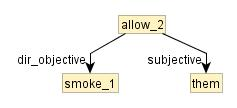
\includegraphics[scale=0.45]{{annexes/figs/test-eval-27.ssynt}.jpg}}
\end{minipage}
\end{tabbing}

\begin{tabbing}
(36)\quad\= \emph{Plays and ballets alternate.} \\
\> \begin{minipage}{16cm}
\raisebox{-0.5\height}{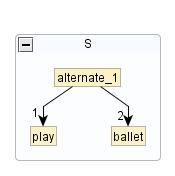
\includegraphics[scale=0.45]{{annexes/figs/test-eval-36.sem}.jpg}}
\raisebox{-0.5\height}{~$\Rightarrow$~}
\raisebox{-0.5\height}{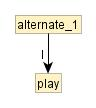
\includegraphics[scale=0.45]{{annexes/figs/test-eval-36.dsynt}.jpg}}
\raisebox{-0.5\height}{~$\Rightarrow$~}
\raisebox{-0.5\height}{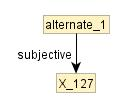
\includegraphics[scale=0.45]{{annexes/figs/test-eval-36.ssynt}.jpg}}
\end{minipage}
\end{tabbing}

\begin{tabbing}
(77)\quad\= \emph{I begged her to do it.} \\
\> \begin{minipage}{16cm}
\raisebox{-0.5\height}{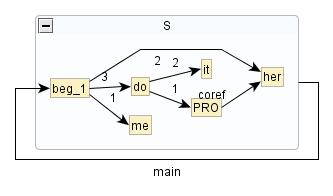
\includegraphics[scale=0.45]{{annexes/figs/test-eval-77.sem}.jpg}}
\raisebox{-0.5\height}{~$\Rightarrow$~}
\raisebox{-0.5\height}{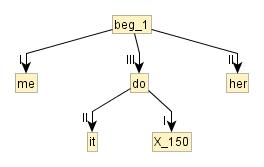
\includegraphics[scale=0.45]{{annexes/figs/test-eval-77.dsynt}.jpg}}
\\
\raisebox{-0.5\height}{~$\Rightarrow$~}
\raisebox{-0.5\height}{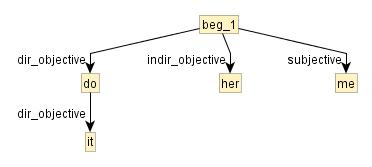
\includegraphics[scale=0.45]{{annexes/figs/test-eval-77.ssynt}.jpg}}
\end{minipage}
\end{tabbing}

\begin{tabbing}
(111)\quad\= \emph{The dragon breathed fire on Mary.} \\
\> \begin{minipage}{16cm}
\raisebox{-0.5\height}{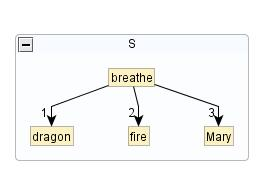
\includegraphics[scale=0.45]{{annexes/figs/test-eval-111.sem}.jpg}}
\raisebox{-0.5\height}{~$\Rightarrow$~}
\raisebox{-0.5\height}{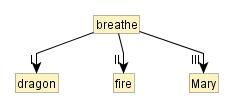
\includegraphics[scale=0.45]{{annexes/figs/test-eval-111.dsynt}.jpg}}
\raisebox{-0.5\height}{~$\Rightarrow$~}
\raisebox{-0.5\height}{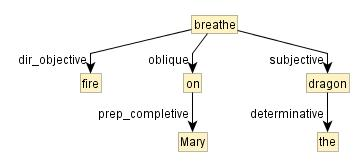
\includegraphics[scale=0.45]{{annexes/figs/test-eval-111.ssynt}.jpg}}
\end{minipage}
\end{tabbing}

\begin{tabbing}
(142)\quad\= \emph{Oils’s price increased ten percent.} \\
\> \begin{minipage}{16cm}
\raisebox{-0.5\height}{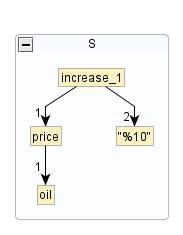
\includegraphics[scale=0.45]{{annexes/figs/test-eval-142.sem}.jpg}}
\raisebox{-0.5\height}{~$\Rightarrow$~}
\raisebox{-0.5\height}{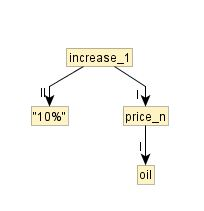
\includegraphics[scale=0.45]{{annexes/figs/test-eval-142.dsynt}.jpg}}
\raisebox{-0.5\height}{~$\Rightarrow$~}
\raisebox{-0.5\height}{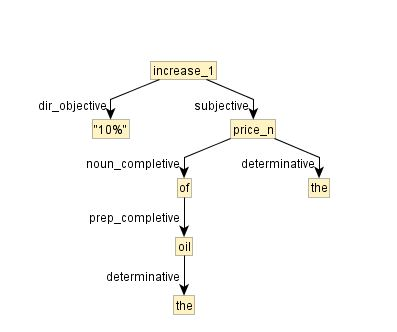
\includegraphics[scale=0.45]{{annexes/figs/test-eval-142.ssynt}.jpg}}
\end{minipage}
\end{tabbing}

\begin{tabbing}
(177)\quad\= \emph{The doctor cured Pat of pneumonia.} \\
\> \begin{minipage}{16cm}
\raisebox{-0.5\height}{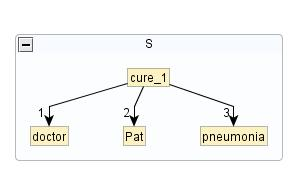
\includegraphics[scale=0.45]{{annexes/figs/test-eval-177.sem}.jpg}}
\raisebox{-0.5\height}{~$\Rightarrow$~}
\raisebox{-0.5\height}{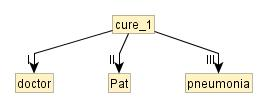
\includegraphics[scale=0.45]{{annexes/figs/test-eval-177.dsynt}.jpg}}
\raisebox{-0.5\height}{~$\Rightarrow$~}
\raisebox{-0.5\height}{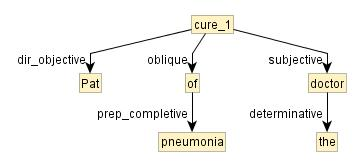
\includegraphics[scale=0.45]{{annexes/figs/test-eval-177.ssynt}.jpg}}
\end{minipage}
\end{tabbing}

\begin{tabbing}
(198)\quad\= \emph{She classified the works as 'dangerous'.} \\
\> \begin{minipage}{16cm}
\raisebox{-0.5\height}{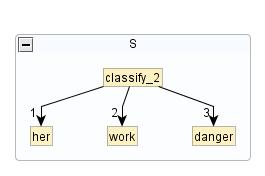
\includegraphics[scale=0.45]{{annexes/figs/test-eval-198.sem}.jpg}}
\raisebox{-0.5\height}{~$\Rightarrow$~}
\raisebox{-0.5\height}{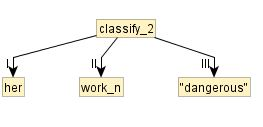
\includegraphics[scale=0.45]{{annexes/figs/test-eval-198.dsynt}.jpg}}
\raisebox{-0.5\height}{~$\Rightarrow$~}
\raisebox{-0.5\height}{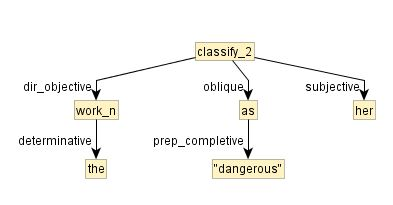
\includegraphics[scale=0.45]{{annexes/figs/test-eval-198.ssynt}.jpg}}
\end{minipage}
\end{tabbing}

\begin{tabbing}
(206)\quad\= \emph{Cora coiled the rope around the post.} \\
\> \begin{minipage}{16cm}
\raisebox{-0.5\height}{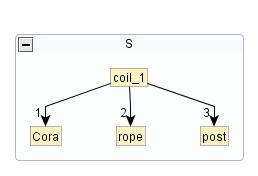
\includegraphics[scale=0.45]{{annexes/figs/test-eval-206.sem}.jpg}}
\raisebox{-0.5\height}{~$\Rightarrow$~}
\raisebox{-0.5\height}{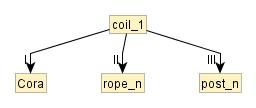
\includegraphics[scale=0.45]{{annexes/figs/test-eval-206.dsynt}.jpg}}
\raisebox{-0.5\height}{~$\Rightarrow$~}
\raisebox{-0.5\height}{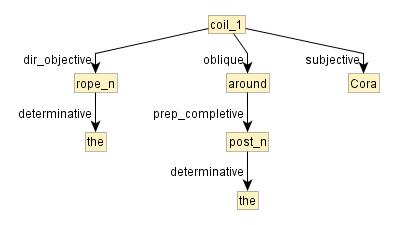
\includegraphics[scale=0.45]{{annexes/figs/test-eval-206.ssynt}.jpg}}
\end{minipage}
\end{tabbing}


\begin{tabbing}
(213)\quad\= \emph{The prime minister complained to the former president about U.S. interference} \\
          \> \emph{in his country’s affairs.} \\
\> \begin{minipage}{16cm}
\raisebox{-0.5\height}{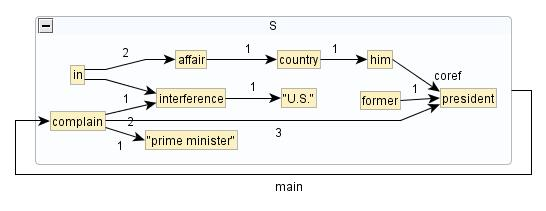
\includegraphics[scale=0.45]{{annexes/figs/test-eval-213.sem}.jpg}}
\raisebox{-0.5\height}{~$\Rightarrow$~}
\raisebox{-0.5\height}{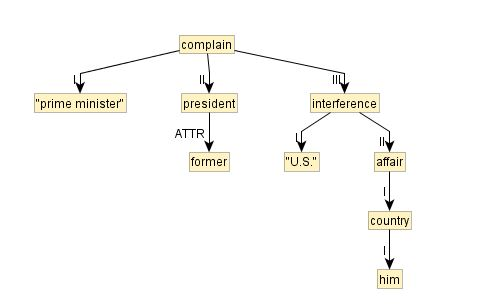
\includegraphics[scale=0.45]{{annexes/figs/test-eval-213.dsynt}.jpg}}
\raisebox{-0.5\height}{~$\Rightarrow$~}
\raisebox{-0.5\height}{\includegraphics[scale=0.45]{{annexes/figs/test-eval-213.ssynt}.jpg}}
\end{minipage}
\end{tabbing}


\begin{tabbing}
(222)\quad\= \emph{The Milky Way comprises more than 100 billion planets.} \\
\> \begin{minipage}{16cm}
\raisebox{-0.5\height}{\includegraphics[scale=0.45]{{annexes/figs/test-eval-222.sem}.jpg}}
\raisebox{-0.5\height}{~$\Rightarrow$~}
\raisebox{-0.5\height}{\includegraphics[scale=0.45]{{annexes/figs/test-eval-222.dsynt}.jpg}}
\raisebox{-0.5\height}{~$\Rightarrow$~}
\raisebox{-0.5\height}{\includegraphics[scale=0.45]{{annexes/figs/test-eval-222.ssynt}.jpg}}
\end{minipage}
\end{tabbing}

\begin{tabbing}
(227)\quad\= \emph{The children hid from Sally.} \\
\> \begin{minipage}{16cm}
\raisebox{-0.5\height}{\includegraphics[scale=0.45]{{annexes/figs/test-eval-227.sem}.jpg}}
\raisebox{-0.5\height}{~$\Rightarrow$~}
\raisebox{-0.5\height}{\includegraphics[scale=0.45]{{annexes/figs/test-eval-227.dsynt}.jpg}}
\raisebox{-0.5\height}{~$\Rightarrow$~}
\raisebox{-0.5\height}{\includegraphics[scale=0.45]{{annexes/figs/test-eval-227.ssynt}.jpg}}
\end{minipage}
\end{tabbing}

\begin{tabbing}
(244)\quad\= \emph{They considered him professor.} \\
\> \begin{minipage}{16cm}
\raisebox{-0.5\height}{\includegraphics[scale=0.45]{{annexes/figs/test-eval-244.sem}.jpg}}
\raisebox{-0.5\height}{~$\Rightarrow$~}
\raisebox{-0.5\height}{\includegraphics[scale=0.45]{{annexes/figs/test-eval-244.dsynt}.jpg}}
\raisebox{-0.5\height}{~$\Rightarrow$~}
\raisebox{-0.5\height}{\includegraphics[scale=0.45]{{annexes/figs/test-eval-244.ssynt}.jpg}}
\end{minipage}
\end{tabbing}

\begin{tabbing}
(250)\quad\= \emph{I spent the time on worries.} \\
\> \begin{minipage}{16cm}
\raisebox{-0.5\height}{\includegraphics[scale=0.45]{{annexes/figs/test-eval-250.sem}.jpg}}
\raisebox{-0.5\height}{~$\Rightarrow$~}
\raisebox{-0.5\height}{\includegraphics[scale=0.45]{{annexes/figs/test-eval-250.dsynt}.jpg}}
\raisebox{-0.5\height}{~$\Rightarrow$~}
\raisebox{-0.5\height}{\includegraphics[scale=0.45]{{annexes/figs/test-eval-250.ssynt}.jpg}}
\end{minipage}
\end{tabbing}

\begin{tabbing}
(264)\quad\= \emph{Some of the members may donate privately.} \\
\> \begin{minipage}{16cm}
\raisebox{-0.5\height}{\includegraphics[scale=0.45]{{annexes/figs/test-eval-264.sem}.jpg}}
\raisebox{-0.5\height}{~$\Rightarrow$~}
\raisebox{-0.5\height}{\includegraphics[scale=0.45]{{annexes/figs/test-eval-264.dsynt}.jpg}}
\raisebox{-0.5\height}{~$\Rightarrow$~}
\raisebox{-0.5\height}{\includegraphics[scale=0.45]{{annexes/figs/test-eval-264.ssynt}.jpg}}
\end{minipage}
\end{tabbing}

\begin{tabbing}
(267)\quad\= \emph{He converted to believing in Buddha.} \\
\> \begin{minipage}{16cm}
\raisebox{-0.5\height}{\includegraphics[scale=0.45]{{annexes/figs/test-eval-267.sem}.jpg}}
\raisebox{-0.5\height}{~$\Rightarrow$~}
\raisebox{-0.5\height}{\includegraphics[scale=0.45]{{annexes/figs/test-eval-267.dsynt}.jpg}}
\raisebox{-0.5\height}{~$\Rightarrow$~}
\raisebox{-0.5\height}{\includegraphics[scale=0.45]{{annexes/figs/test-eval-267.ssynt}.jpg}}
\end{minipage}
\\
\> \draft{Bla bla le noeud X...}
\end{tabbing}



\begin{tabbing}
(330)\quad\= \emph{This flyer and that flyer differ.} \\
\> \begin{minipage}{16cm}
\raisebox{-0.5\height}{\includegraphics[scale=0.45]{{annexes/figs/test-eval-330.sem}.jpg}}
\raisebox{-0.5\height}{~$\Rightarrow$~}
%\raisebox{-0.5\height}{\includegraphics[scale=0.45]{{annexes/figs/test-eval-330.dsynt}.jpg}}
\raisebox{-0.5\height}{~$\Rightarrow$~}
%\raisebox{-0.5\height}{\includegraphics[scale=0.45]{{annexes/figs/test-eval-330.ssynt}.jpg}}
\end{minipage}
\end{tabbing}

\begin{tabbing}
(384)\quad\= \emph{He entered the room.} \\
\> \begin{minipage}{16cm}
\raisebox{-0.5\height}{\includegraphics[scale=0.45]{{annexes/figs/test-eval-384.sem}.jpg}}
\raisebox{-0.5\height}{~$\Rightarrow$~}
\raisebox{-0.5\height}{\includegraphics[scale=0.45]{{annexes/figs/test-eval-384.dsynt}.jpg}}
\raisebox{-0.5\height}{~$\Rightarrow$~}
\raisebox{-0.5\height}{\includegraphics[scale=0.45]{{annexes/figs/test-eval-384.ssynt}.jpg}}
\end{minipage}
\end{tabbing}

\begin{tabbing}
(399)\quad\= \emph{The bells traded places.} \\
\> \begin{minipage}{16cm}
\raisebox{-0.5\height}{\includegraphics[scale=0.45]{{annexes/figs/test-eval-399.sem}.jpg}}
\raisebox{-0.5\height}{~$\Rightarrow$~}
\raisebox{-0.5\height}{\includegraphics[scale=0.45]{{annexes/figs/test-eval-399.dsynt}.jpg}}
\raisebox{-0.5\height}{~$\Rightarrow$~}
\raisebox{-0.5\height}{\includegraphics[scale=0.45]{{annexes/figs/test-eval-399.ssynt}.jpg}}
\end{minipage}
\end{tabbing}


\begin{tabbing}
(426)\quad\= \emph{We focused on it.} \\
\> \begin{minipage}{16cm}
\raisebox{-0.5\height}{\includegraphics[scale=0.45]{{annexes/figs/test-eval-426.sem}.jpg}}
\raisebox{-0.5\height}{~$\Rightarrow$~}
\raisebox{-0.5\height}{\includegraphics[scale=0.45]{{annexes/figs/test-eval-426.dsynt}.jpg}}
\raisebox{-0.5\height}{~$\Rightarrow$~}
\raisebox{-0.5\height}{\includegraphics[scale=0.45]{{annexes/figs/test-eval-426.ssynt}.jpg}}
\end{minipage}
\end{tabbing}

\begin{tabbing}
(428)\quad\= \emph{We brooded about it.} \\
\> \begin{minipage}{16cm}
\raisebox{-0.5\height}{\includegraphics[scale=0.45]{{annexes/figs/test-eval-428.sem}.jpg}}
\raisebox{-0.5\height}{~$\Rightarrow$~}
\raisebox{-0.5\height}{\includegraphics[scale=0.45]{{annexes/figs/test-eval-428.dsynt}.jpg}}
\raisebox{-0.5\height}{~$\Rightarrow$~}
\raisebox{-0.5\height}{\includegraphics[scale=0.45]{{annexes/figs/test-eval-428.ssynt}.jpg}}
\end{minipage}
\end{tabbing}

\begin{tabbing}
(452)\quad\= \emph{Carmen bought a dress for 50\$.} \\
\> \begin{minipage}{16cm}
\raisebox{-0.5\height}{\includegraphics[scale=0.45]{{annexes/figs/test-eval-452.sem}.jpg}}
\raisebox{-0.5\height}{~$\Rightarrow$~}
\raisebox{-0.5\height}{\includegraphics[scale=0.45]{{annexes/figs/test-eval-452.dsynt}.jpg}}
\raisebox{-0.5\height}{~$\Rightarrow$~}
\raisebox{-0.5\height}{\includegraphics[scale=0.45]{{annexes/figs/test-eval-452.ssynt}.jpg}}
\end{minipage}
\end{tabbing}

\begin{tabbing}
(476)\quad\= \emph{The teacher gathered the kids.} \\
\> \begin{minipage}{16cm}
\raisebox{-0.5\height}{\includegraphics[scale=0.45]{{annexes/figs/test-eval-476.sem}.jpg}}
\raisebox{-0.5\height}{~$\Rightarrow$~}
\raisebox{-0.5\height}{\includegraphics[scale=0.45]{{annexes/figs/test-eval-476.dsynt}.jpg}}
\raisebox{-0.5\height}{~$\Rightarrow$~}
\raisebox{-0.5\height}{\includegraphics[scale=0.45]{{annexes/figs/test-eval-476.ssynt}.jpg}}
\end{minipage}
\end{tabbing}

\begin{tabbing}
(503)\quad\= \emph{Smith was inscribing.} \\
\> \begin{minipage}{16cm}
\raisebox{-0.5\height}{\includegraphics[scale=0.45]{{annexes/figs/test-eval-503.sem}.jpg}}
\raisebox{-0.5\height}{~$\Rightarrow$~}
\raisebox{-0.5\height}{\includegraphics[scale=0.45]{{annexes/figs/test-eval-503.dsynt}.jpg}}
\raisebox{-0.5\height}{~$\Rightarrow$~}
\raisebox{-0.5\height}{\includegraphics[scale=0.45]{{annexes/figs/test-eval-503.ssynt}.jpg}}
\end{minipage}
\end{tabbing}


\begin{tabbing}
(540)\quad\= \emph{We abandoned the area.} \\
\> \begin{minipage}{16cm}
\raisebox{-0.5\height}{\includegraphics[scale=0.45]{{annexes/figs/test-eval-540.sem}.jpg}}
\raisebox{-0.5\height}{~$\Rightarrow$~}
\raisebox{-0.5\height}{\includegraphics[scale=0.45]{{annexes/figs/test-eval-540.dsynt}.jpg}}
\raisebox{-0.5\height}{~$\Rightarrow$~}
\raisebox{-0.5\height}{\includegraphics[scale=0.45]{{annexes/figs/test-eval-540.ssynt}.jpg}}
\end{minipage}
\end{tabbing}

\begin{tabbing}
(554)\quad\= \emph{Sasha dawdled in the museum.} \\
\> \begin{minipage}{16cm}
\raisebox{-0.5\height}{\includegraphics[scale=0.45]{{annexes/figs/test-eval-554.sem}.jpg}}
\raisebox{-0.5\height}{~$\Rightarrow$~}
\raisebox{-0.5\height}{\includegraphics[scale=0.45]{{annexes/figs/test-eval-554.dsynt}.jpg}}
\raisebox{-0.5\height}{~$\Rightarrow$~}
\raisebox{-0.5\height}{\includegraphics[scale=0.45]{{annexes/figs/test-eval-554.ssynt}.jpg}}
\end{minipage}
\end{tabbing}

\begin{tabbing}
(581)\quad\= \emph{I anguished over Aslan’s pain.} \\
\> \begin{minipage}{16cm}
\raisebox{-0.5\height}{\includegraphics[scale=0.45]{{annexes/figs/test-eval-581.sem}.jpg}}
\raisebox{-0.5\height}{~$\Rightarrow$~}
\raisebox{-0.5\height}{\includegraphics[scale=0.45]{{annexes/figs/test-eval-581.dsynt}.jpg}}
\raisebox{-0.5\height}{~$\Rightarrow$~}
\raisebox{-0.5\height}{\includegraphics[scale=0.45]{{annexes/figs/test-eval-581.ssynt}.jpg}}
\end{minipage}
\end{tabbing}

\begin{tabbing}
(583)\quad\= \emph{Dina masqueraded as a lawyer.} \\
\> \begin{minipage}{16cm}
\raisebox{-0.5\height}{\includegraphics[scale=0.45]{{annexes/figs/test-eval-583.sem}.jpg}}
\raisebox{-0.5\height}{~$\Rightarrow$~}
\raisebox{-0.5\height}{\includegraphics[scale=0.45]{{annexes/figs/test-eval-583.dsynt}.jpg}}
\raisebox{-0.5\height}{~$\Rightarrow$~}
\raisebox{-0.5\height}{\includegraphics[scale=0.45]{{annexes/figs/test-eval-583.ssynt}.jpg}}
\end{minipage}
\end{tabbing}


\begin{tabbing}
(604)\quad\= \emph{Herman added a computer to the network.} \\
\> \begin{minipage}{16cm}
\raisebox{-0.5\height}{\includegraphics[scale=0.45]{{annexes/figs/test-eval-604.sem}.jpg}}
\raisebox{-0.5\height}{~$\Rightarrow$~}
\raisebox{-0.5\height}{\includegraphics[scale=0.45]{{annexes/figs/test-eval-604.dsynt}.jpg}}
\raisebox{-0.5\height}{~$\Rightarrow$~}
\raisebox{-0.5\height}{\includegraphics[scale=0.45]{{annexes/figs/test-eval-604.ssynt}.jpg}}
\end{minipage}
\end{tabbing}

\begin{tabbing}
(618)\quad\= \emph{I neglected to do the job.} \\
\> \begin{minipage}{16cm}
\raisebox{-0.5\height}{\includegraphics[scale=0.45]{{annexes/figs/test-eval-618.sem}.jpg}}
\raisebox{-0.5\height}{~$\Rightarrow$~}
\raisebox{-0.5\height}{\includegraphics[scale=0.45]{{annexes/figs/test-eval-618.dsynt}.jpg}}
\raisebox{-0.5\height}{~$\Rightarrow$~}
\raisebox{-0.5\height}{\includegraphics[scale=0.45]{{annexes/figs/test-eval-618.ssynt}.jpg}}
\end{minipage}
\end{tabbing}

\begin{tabbing}
(630)\quad\= \emph{She laughed in embarrassment.} \\
\> \begin{minipage}{16cm}
\raisebox{-0.5\height}{\includegraphics[scale=0.45]{{annexes/figs/test-eval-630.sem}.jpg}}
\raisebox{-0.5\height}{~$\Rightarrow$~}
%\raisebox{-0.5\height}{\includegraphics[scale=0.45]{{annexes/figs/test-eval-630.dsynt}.jpg}}
\raisebox{-0.5\height}{~$\Rightarrow$~}
%\raisebox{-0.5\height}{\includegraphics[scale=0.45]{{annexes/figs/test-eval-630.ssynt}.jpg}}
\end{minipage}
\end{tabbing}

\begin{tabbing}
(667)\quad\= \emph{Lydia pocketed the change in her left pocket.} \\
\> \begin{minipage}{16cm}
\raisebox{-0.5\height}{\includegraphics[scale=0.45]{{annexes/figs/test-eval-667.sem}.jpg}}
\raisebox{-0.5\height}{~$\Rightarrow$~}
\raisebox{-0.5\height}{\includegraphics[scale=0.45]{{annexes/figs/test-eval-667.dsynt}.jpg}}
\raisebox{-0.5\height}{~$\Rightarrow$~}
\raisebox{-0.5\height}{\includegraphics[scale=0.45]{{annexes/figs/test-eval-667.ssynt}.jpg}}
\end{minipage}
\end{tabbing}

\begin{tabbing}
(686)\quad\= \emph{Donna grilled me steaks.} \\

\> \begin{minipage}{16cm}
\raisebox{-0.5\height}{\includegraphics[scale=0.45]{{annexes/figs/test-eval-686.sem}.jpg}}
\raisebox{-0.5\height}{~$\Rightarrow$~}
\raisebox{-0.5\height}{\includegraphics[scale=0.45]{{annexes/figs/test-eval-686.dsynt}.jpg}}
\raisebox{-0.5\height}{~$\Rightarrow$~}
\raisebox{-0.5\height}{\includegraphics[scale=0.45]{{annexes/figs/test-eval-686.ssynt}.jpg}}
\end{minipage}
\end{tabbing}

\begin{tabbing}
(688)\quad\= \emph{The dealer valued the book.} \\
\> \begin{minipage}{16cm}
\raisebox{-0.5\height}{\includegraphics[scale=0.45]{{annexes/figs/test-eval-688.sem}.jpg}}
\raisebox{-0.5\height}{~$\Rightarrow$~}
\raisebox{-0.5\height}{\includegraphics[scale=0.45]{{annexes/figs/test-eval-688.dsynt}.jpg}}
\raisebox{-0.5\height}{~$\Rightarrow$~}
\raisebox{-0.5\height}{\includegraphics[scale=0.45]{{annexes/figs/test-eval-688.ssynt}.jpg}}
\end{minipage}
\end{tabbing}


\begin{tabbing}
(746)\quad\= \emph{Tom jumped the horse over the fence.} \\
\> \begin{minipage}{16cm}
\raisebox{-0.5\height}{\includegraphics[scale=0.45]{{annexes/figs/test-eval-746.sem}.jpg}}
\raisebox{-0.5\height}{~$\Rightarrow$~}
\raisebox{-0.5\height}{\includegraphics[scale=0.45]{{annexes/figs/test-eval-746.dsynt}.jpg}}
\raisebox{-0.5\height}{~$\Rightarrow$~}
\raisebox{-0.5\height}{\includegraphics[scale=0.45]{{annexes/figs/test-eval-746.ssynt}.jpg}}
\end{minipage}
\end{tabbing}


\begin{tabbing}
(750)\quad\= \emph{The horse jumped the stream.} \\
\> \begin{minipage}{16cm}
\raisebox{-0.5\height}{\includegraphics[scale=0.45]{{annexes/figs/test-eval-750.sem}.jpg}}
\raisebox{-0.5\height}{~$\Rightarrow$~}
\raisebox{-0.5\height}{\includegraphics[scale=0.45]{{annexes/figs/test-eval-750.dsynt}.jpg}}
\raisebox{-0.5\height}{~$\Rightarrow$~}
\raisebox{-0.5\height}{\includegraphics[scale=0.45]{{annexes/figs/test-eval-750.ssynt}.jpg}}
\end{minipage}
\end{tabbing}

\begin{tabbing}
(777)\quad\= \emph{TransCanada is shifting its HQ to Calgary from Toronto.} \\
\> \begin{minipage}{16cm}
\raisebox{-0.5\height}{\includegraphics[scale=0.45]{{annexes/figs/test-eval-777.sem}.jpg}}
\raisebox{-0.5\height}{~$\Rightarrow$~}
\raisebox{-0.5\height}{\includegraphics[scale=0.45]{{annexes/figs/test-eval-777.dsynt}.jpg}}
\raisebox{-0.5\height}{~$\Rightarrow$~}
\raisebox{-0.5\height}{\includegraphics[scale=0.45]{{annexes/figs/test-eval-777.ssynt}.jpg}}
\end{minipage}
\end{tabbing}

\begin{tabbing}
(789)\quad\= \emph{The crew spotted the island.} \\
\> \begin{minipage}{16cm}
\raisebox{-0.5\height}{\includegraphics[scale=0.45]{{annexes/figs/test-eval-789.sem}.jpg}}
\raisebox{-0.5\height}{~$\Rightarrow$~}
\raisebox{-0.5\height}{\includegraphics[scale=0.45]{{annexes/figs/test-eval-789.dsynt}.jpg}}
\raisebox{-0.5\height}{~$\Rightarrow$~}
\raisebox{-0.5\height}{\includegraphics[scale=0.45]{{annexes/figs/test-eval-789.ssynt}.jpg}}
\end{minipage}
\end{tabbing}

\begin{tabbing}
(836)\quad\= \emph{The thief stole the paint for Mary.} \\
\> \begin{minipage}{16cm}
%\raisebox{-0.5\height}{\includegraphics[scale=0.45]{{annexes/figs/test-eval-836.sem}.jpg}}
\raisebox{-0.5\height}{~$\Rightarrow$~}
%\raisebox{-0.5\height}{\includegraphics[scale=0.45]{{annexes/figs/test-eval-836.dsynt}.jpg}}
\raisebox{-0.5\height}{~$\Rightarrow$~}
%\raisebox{-0.5\height}{\includegraphics[scale=0.45]{{annexes/figs/test-eval-836.ssynt}.jpg}}
\end{minipage}
\end{tabbing}


\begin{tabbing}
(843)\quad\= \emph{I ended the party with a speech.} \\
\> \begin{minipage}{16cm}
\raisebox{-0.5\height}{\includegraphics[scale=0.45]{{annexes/figs/test-eval-843.sem}.jpg}}
\raisebox{-0.5\height}{~$\Rightarrow$~}
\raisebox{-0.5\height}{\includegraphics[scale=0.45]{{annexes/figs/test-eval-843.dsynt}.jpg}}
\raisebox{-0.5\height}{~$\Rightarrow$~}
\raisebox{-0.5\height}{\includegraphics[scale=0.45]{{annexes/figs/test-eval-843.ssynt}.jpg}}
\end{minipage}
\end{tabbing}

\begin{tabbing}
(845)\quad\= \emph{Winnie the Pooh subjugated the unfortunate Pixies.} \\
\> \begin{minipage}{16cm}
\raisebox{-0.5\height}{\includegraphics[scale=0.45]{{annexes/figs/test-eval-845.sem}.jpg}}
\raisebox{-0.5\height}{~$\Rightarrow$~}
\raisebox{-0.5\height}{\includegraphics[scale=0.45]{{annexes/figs/test-eval-845.dsynt}.jpg}}
\raisebox{-0.5\height}{~$\Rightarrow$~}
\raisebox{-0.5\height}{\includegraphics[scale=0.45]{{annexes/figs/test-eval-845.ssynt}.jpg}}
\end{minipage}
\end{tabbing}


\begin{tabbing}
(851)\quad\= \emph{The streets gushed with water.} \\
\> \begin{minipage}{16cm}
\raisebox{-0.5\height}{\includegraphics[scale=0.45]{{annexes/figs/test-eval-851.sem}.jpg}}
\raisebox{-0.5\height}{~$\Rightarrow$~}
\raisebox{-0.5\height}{\includegraphics[scale=0.45]{{annexes/figs/test-eval-851.dsynt}.jpg}}
\raisebox{-0.5\height}{~$\Rightarrow$~}
\raisebox{-0.5\height}{\includegraphics[scale=0.45]{{annexes/figs/test-eval-851.ssynt}.jpg}}
\end{minipage}
\end{tabbing}

\begin{tabbing}
(862)\quad\= \emph{The sailor drowned.} \\
\> \begin{minipage}{16cm}
\raisebox{-0.5\height}{\includegraphics[scale=0.45]{{annexes/figs/test-eval-862.sem}.jpg}}
\raisebox{-0.5\height}{~$\Rightarrow$~}
\raisebox{-0.5\height}{\includegraphics[scale=0.45]{{annexes/figs/test-eval-862.dsynt}.jpg}}
\raisebox{-0.5\height}{~$\Rightarrow$~}
\raisebox{-0.5\height}{\includegraphics[scale=0.45]{{annexes/figs/test-eval-862.ssynt}.jpg}}
\end{minipage}
\end{tabbing}

\begin{tabbing}
(868)\quad\= \emph{Bees are swarming in the garden.} \\
\> \begin{minipage}{16cm}
\raisebox{-0.5\height}{\includegraphics[scale=0.45]{{annexes/figs/test-eval-868.sem}.jpg}}
\raisebox{-0.5\height}{~$\Rightarrow$~}
\raisebox{-0.5\height}{\includegraphics[scale=0.45]{{annexes/figs/test-eval-868.dsynt}.jpg}}
\raisebox{-0.5\height}{~$\Rightarrow$~}
\raisebox{-0.5\height}{\includegraphics[scale=0.45]{{annexes/figs/test-eval-868.ssynt}.jpg}}
\end{minipage}
\end{tabbing}

\begin{tabbing}
(873)\quad\= \emph{Paula swatted the fly with a cloth.} \\
\> \begin{minipage}{16cm}
\raisebox{-0.5\height}{\includegraphics[scale=0.45]{{annexes/figs/test-eval-873.sem}.jpg}}
\raisebox{-0.5\height}{~$\Rightarrow$~}
\raisebox{-0.5\height}{\includegraphics[scale=0.45]{{annexes/figs/test-eval-873.dsynt}.jpg}}
\raisebox{-0.5\height}{~$\Rightarrow$~}
\raisebox{-0.5\height}{\includegraphics[scale=0.45]{{annexes/figs/test-eval-873.ssynt}.jpg}}
\end{minipage}
\end{tabbing}

\begin{tabbing}
(894)\quad\= \emph{Ellen told me a story.} \\
\> \begin{minipage}{16cm}
\raisebox{-0.5\height}{\includegraphics[scale=0.45]{{annexes/figs/test-eval-894.sem}.jpg}}
\raisebox{-0.5\height}{~$\Rightarrow$~}
\raisebox{-0.5\height}{\includegraphics[scale=0.45]{{annexes/figs/test-eval-894.dsynt}.jpg}}
\raisebox{-0.5\height}{~$\Rightarrow$~}
\raisebox{-0.5\height}{\includegraphics[scale=0.45]{{annexes/figs/test-eval-894.ssynt}.jpg}}
\end{minipage}
\end{tabbing}

\begin{tabbing}
(900)\quad\= \emph{Steve tossed the ball from the corner to the garden.} \\
\> \begin{minipage}{16cm}
\raisebox{-0.5\height}{\includegraphics[scale=0.45]{{annexes/figs/test-eval-900.sem}.jpg}}
\raisebox{-0.5\height}{~$\Rightarrow$~}
\raisebox{-0.5\height}{\includegraphics[scale=0.45]{{annexes/figs/test-eval-900.dsynt}.jpg}}
\raisebox{-0.5\height}{~$\Rightarrow$~}
\raisebox{-0.5\height}{\includegraphics[scale=0.45]{{annexes/figs/test-eval-900.ssynt}.jpg}}
\end{minipage}
\end{tabbing}

\begin{tabbing}
(955)\quad\= \emph{Linda winked her eye.} \\
\> \begin{minipage}{16cm}
\raisebox{-0.5\height}{\includegraphics[scale=0.45]{{annexes/figs/test-eval-955.sem}.jpg}}
\raisebox{-0.5\height}{~$\Rightarrow$~}
\raisebox{-0.5\height}{\includegraphics[scale=0.45]{{annexes/figs/test-eval-955.dsynt}.jpg}}
\raisebox{-0.5\height}{~$\Rightarrow$~}
\raisebox{-0.5\height}{\includegraphics[scale=0.45]{{annexes/figs/test-eval-955.ssynt}.jpg}}
\end{minipage}
\end{tabbing}

\begin{tabbing}
(968)\quad\= \emph{Barry Cryer erased the writing.} \\
\> \begin{minipage}{16cm}
\raisebox{-0.5\height}{\includegraphics[scale=0.45]{{annexes/figs/test-eval-968.sem}.jpg}}
\raisebox{-0.5\height}{~$\Rightarrow$~}
\raisebox{-0.5\height}{\includegraphics[scale=0.45]{{annexes/figs/test-eval-968.dsynt}.jpg}}
\raisebox{-0.5\height}{~$\Rightarrow$~}
\raisebox{-0.5\height}{\includegraphics[scale=0.45]{{annexes/figs/test-eval-968.ssynt}.jpg}}
\end{minipage}
\end{tabbing}


\begin{tabbing}
(974)\quad\= \emph{He backed out of going on the trip.} \\
\> \begin{minipage}{16cm}
\raisebox{-0.5\height}{\includegraphics[scale=0.45]{{annexes/figs/test-eval-974.sem}.jpg}}
\raisebox{-0.5\height}{~$\Rightarrow$~}
%\raisebox{-0.5\height}{\includegraphics[scale=0.45]{{annexes/figs/test-eval-974.dsynt}.jpg}}
\raisebox{-0.5\height}{~$\Rightarrow$~}
%\raisebox{-0.5\height}{\includegraphics[scale=0.45]{{annexes/figs/test-eval-974.ssynt}.jpg}}
\end{minipage}
\end{tabbing}
\chapter{Inputs et outputs}

Voici les inputs et outputs provenant des phrases tirées de VerbNet

\begin{enumerate}
 % \item Structure sémantique 17
	\begin{figure}[htb]
	\centering
	\includegraphics[width=0.3\textwidth, trim = {0cm 0cm 0cm 0cm},clip]{annexes/figs/{test-eval-1.sem}.jpg}
	\caption{Structure sémantique 17}
	\label{fig:str17sem}
\end{figure}
	
\item Structure syntaxique 17.1
	\begin{figure}[htb]
	\centering
	\includegraphics[width=0.4\textwidth, trim = {0cm 0cm 0cm 0cm},clip]{annexes/figs/{test-eval-1.dsynt1.ssynt1}.jpg}
	\caption{I loved writing}
	\label{fig:str17sem}
\end{figure}

\item Structure syntaxique 17.2
	\begin{figure}[htb]
	\centering
	\includegraphics[width=0.4\textwidth, trim = {0cm 0cm 0cm 0cm},clip]{annexes/figs/{test-eval-1.dsynt2.ssynt1}.jpg}
	\caption{I loved writing}
	\label{fig:str17sem}
\end{figure}

\item Structure syntaxique 17.3
	\begin{figure}[htb]
	\centering
	\includegraphics[width=0.4\textwidth, trim = {0cm 0cm 0cm 0cm},clip]{annexes/figs/{test-eval-1.dsynt3.ssynt1}.jpg}
	\caption{I loved writing}
	\label{fig:str17sem}
\end{figure}

\item Structure syntaxique 17.4
	\begin{figure}[htb]
	\centering
	\includegraphics[width=0.4\textwidth, trim = {0cm 0cm 0cm 0cm},clip]{annexes/figs/{test-eval-1.dsynt4.ssynt1}.jpg}
	\caption{I loved writing}
	\label{fig:str17sem}
\end{figure}
\end{enumerate}

\end{document}
